
\documentclass[twocolumn]{article}
\usepackage[english]{babel}
\usepackage[utf8]{inputenc}
\usepackage{amsmath}
\usepackage{centernot}
\usepackage{amsfonts}
\usepackage{subcaption}
\usepackage{mathtools}
\usepackage{graphicx}
\usepackage{color}
\usepackage{authblk}
\usepackage{url}
\usepackage{amssymb}


\usepackage[colorlinks,citecolor=blue,linkcolor=blue,urlcolor=blue,bookmarks=false,hypertexnames=true]{hyperref}
\usepackage{geometry}
\graphicspath{{images/}}

% Margins:
\geometry{
	a4paper,
	total={170mm,257mm},
	left=20mm,
	right=20mm,
	top=20mm,
	bottom=20mm,
}

\def\UrlBreaks{\do\/\do-}

%\usepackage[ruled]{algorithm2e}
%
%
%\makeatletter
%\newcommand{\RemoveAlgoNumber}{\renewcommand{\fnum@algocf}{\AlCapSty{\AlCapFnt\algorithmcfname}}}
%\newcommand{\RevertAlgoNumber}{\algocf@resetfnum}
%\makeatother
%
%%\renewcommand*{\listalgorithmcfname}{List of Heuristics}
%\renewcommand*{\algorithmcfname}{SPEEDY}
%%\renewcommand*{\algorithmautorefname}{heuristic}
%
%


\usepackage{listings}

\definecolor{dkgreen}{rgb}{0,0.6,0}
\definecolor{gray}{rgb}{0.5,0.5,0.5}
\definecolor{mauve}{rgb}{0.58,0,0.82}
\lstset{frame=tb,
	language=Fortran,
	aboveskip=3mm,
	belowskip=3mm,
	showstringspaces=false,
	columns=flexible,
	basicstyle={\small\ttfamily},
	numbers=none,	
	numberstyle=\tiny\color{gray},
	keywordstyle=\color{blue},
	commentstyle=\color{dkgreen},
	stringstyle=\color{mauve},
	breaklines=true,
	breakatwhitespace=true,
	tabsize=3
}


\date{}




% Title stuff
\title{Deep Learning for Verification of Earth-System Parametrisation of Water Bodies}
%\author{Kimpson, Choulga, Chantry, Palmer, others etc.}
%\affil{\small \textit{Oxford, ECMWF,etc.} \normalsize}


\author[Kimpson et al.]{
	Tom Kimpson,$^{1}$\thanks{E-mail: tom.kimpson@physics.ox.ac.uk}
	Margarita Choulga, $^2$
	Matthew Chantry,$^2$
		Gianpaolo Balsamo,$^2$
	Souhail Boussetta,$^2$
		Peter Dueben,$^2$
	and Tim Palmer $^1$ 
	\\
	% List of institutions
	$^{1}$ \small Department of Physics, University of Oxford, Oxford, UK, \\ \normalsize
	$^{2}$ \small Research Department, European Centre for Medium-Range Weather Forecasts (ECMWF), Reading, UK\normalsize
}






\begin{document}
%\RemoveAlgoNumber

\maketitle        


\begin{abstract}
About 2/3 of all densely populated areas (i.e. at least 300 inhabitants per km$^2$) around the globe are situated within a 9 km radius of a permanent waterbody (i.e. inland water or sea/ocean coast), since inland water sustains the vast majority of human activities. Water bodies exchange mass and energy with the atmosphere and need to be accurately simulated in numerical weather prediction and climate modelling as they strongly influence the lower boundary conditions such as skin temperatures, turbulent latent and sensible heat fluxes and moisture availability near the surface. All the non-ocean water (resolved and sub-grid lakes and coastal waters) are represented in the Integrated Forecasting System (IFS) of the European Centre for Medium-Range Weather Forecasts (ECMWF) model, by the Fresh-water Lake (FLake) parametrisation, which treats $\sim$ 1/3 of the land. It is a continuous enterprise to update the surface parametrization schemes and their input fields to better represent small-scale processes. It is, however, difficult to quickly determine both the accuracy of an updated parametrisation, and the added value gained for the purposes of numerical modelling. The aim of our work is to quickly and automatically assess the benefits of an updated lake parametrisation making use of a neural network regression model trained to simulate satellite observed surface skin temperatures. We deploy this tool to determine the accuracy of recent upgrades to the FLake parametrisation, namely the improved permanent lake cover and the capacity to represent seasonally varying water bodies (i.e. ephemeral lakes). We show that for grid-cells where the lake fields have been updated, the prediction accuracy in the land surface temperature improves by 0.45 K on average, whilst for the subset of points where the lakes have been exchanged for bare ground (or vice versa) the improvement is 1.12 K. We also show that updates to the glacier cover improve further the prediction accuracy by 0.14 K. The inclusion of seasonal water is shown to be particularly effective for grid points which are highly time variable, generally improving the simulation accuracy by $\sim$1 K. The neural network regression model has proven to be useful and easily adaptable to assess unforeseen impacts of ancillary datasets, also detecting inappropriate changes of high vegetation to bare ground, which would lead to decreased the skin temperature simulation accuracy by 0.49 K, proving to be a valuable support to model development.
\end{abstract}


\section{Introduction}  %% \introduction[modified heading if necessary]
Globally, there are $\sim$ 117 million lakes - defined as inland water bodies without lateral movement of water - making up around 3.7$\%$ of the Earth's land surface\cite{Verpoorter2014}. Their distribution is highly anisotropic, with the majority of lakes located between $45-75^{\circ}$N in the Boreal and Arctic regions. Lakes are highly important from the perspective of both numerical weather prediction and climate modelling.  For the latter, lakes generally influence the global carbon cycle as both sinks and sources of greenhouse gases; the majority of lakes are net heterotrophic, over saturated with CO$_2$ as a result of in lake respiration and so emit carbon into the atmosphere\cite{Pace2005,Tranvik2009}.  Total CO$_2$ emission from lakes is estimated at $1.25 - 2.30$ Pg of CO2-equivalents annually\cite{DelSontro2018}, nearly $20 \%$ of global CO$_2$ fossil fuel emissions, whilst lakes account for 9-24 $\%$  of CH$_4$ emissions, the second largest natural source after wetlands\cite{Saunois2020}. These rates of greenhouse gas emission are expected to rise further if the eutrophication of the Earth's lentic systems continues. With regards to weather, freezing and melting of the lake surface modifies the radiative and conductive properties and consequently affects the heat (latent, sensible) exchange and surface energy balance\cite{Huang2019,Peng2020,Franz2018}. Considering particular examples, over Lake Victoria convective activity is suppressed during the day and peaks at night, leading to intense, hazardous thunderstorms\cite{Thiery2015,Thiery_2017}; Lake Ladoga can generate low level clouds which can cause variability in the 2m temperature of up to 10 K\cite{Eerola2014}; the Laurentian Great Lakes can cause intense winter snow storms\cite{Vavrus2013} \cite{Notaro2013}. Moreover, as a result of the increased temperatures due to climate change, lakes become more numerous due to the melting of glaciers and permafrost. Additionally, the higher temperatures mean that previously permanent lake bodies become seasonal or intermittent. There is then evidently a huge potential return in the ability to accurately model the location, morphology and properties of lakes in weather and climate models. \newline 


\noindent The Integrated Forecasting System (IFS) at the European Centre for Medium Range Weather Forecasts (ECMWF) is used operationally for numerical weather prediction and climate modelling. Earth-system modelling in the IFS can be broadly categorised into large-scale and small-scale processes. Large-scale processes can be described by numerically solving the relevant set of differential equations, to determine e.g. the general circulation of atmosphere. Conversely, small-scale processes such as clouds or land-surface processes are represented via parametrisation. Accurate parametrisations are essential for the overall accuracy of the model. For example, the parametrisation of the land surface determines the sensible and latent heat fluxes, providing the lower boundary conditions for the equations of enthalpy and moisture in the atmosphere\cite{p16960}. \newline 

\noindent Lakes are incorporated in Earth-system models via parametrisation. At ECMWF the  representation of lakes via parametrisation was first handled by introducing the Fresh water Lake model FLake\cite{Mironov2008} into the IFS. FLake treats all resolved inland waterbodies (i.e. lakes, reservoirs, rivers which are dominating in a grid-cell) and unresolved or sub-grid water (i.e. small inland waterbodies and sea/ocean coastal waters which are present but not dominating in a grid-cell). Note that lake parameters are also an important part of the FLake model so when we refer in this work to ``lake parametrisation" we mean both the model and the parameters. The broad impact of the FLake model and the important role that waterbodies play in human life can be illustrated by analysing ECMWF maps of the fractional land sea mask and the inland waterbody cover alongside maps of the population density (i.e. inhabitants per km$^2$) based on the population count for 2015 from the Global Human Settlement Layers (GHSL), Population Grid 1975-2030\cite{GHS,JRC100523} at 9 km horizontal resolution. Globally FLake is active over 11.1\% of the grid-cells, with only 1.2\% of them being resolved inland waters (i.e. water covers $\geq$50\% of the grid-cell); considering only non-ocean (i.e. land) grid-cells, then FLake is active over 32.4\% of the grid-cells with only 3.5\% of them being resolved waters. According to the population data, only 4\% of land is densely populated (i.e. at least 300 inhabitants per km$^2$); 64.5\% of these areas being situated within a 9 km radius of a permanent waterbody (i.e. inland water or sea/ocean coast) with half of it (i.e. 31.2\% of densely populated areas) being in the vicinity of at least 1 km$^2$ waterbody - emphasising how essential waterbodies are in human life. In some regions this role may be even more crucial than in the others. For example, only 2\% of the North American region (similar for South American and North Asian regions) is densely populated with 45.7\% (33.9\% and 37.9\% respectively) of the areas being in vicinity of at least 1 km$^2$ waterbody; for Europe even though it has more densely populated areas (16\% of land is densely populated) still 37.4\% of the population are in the vicinity of at least a 1 km$^2$ waterbody; for a rather dry continent like Africa only 5\% of land is densely populated with 22.2\% of these areas being close to at least a 1 km$^2$ waterbody; most striking in this sense is Australia where only 0.5 \% of the land is populated, with two thirds of the population living within 9 km radius of a permanent waterbody of at least 1 km$^2$, with the majority of people living on the ocean coast. \newline 

\noindent It is a continuous enterprise to update the lake parametrization schemes and their input data fields to better represent small-scale surface processes. It is however challenging to accurately represent lakes in these parametrisations; the majority of lakes which are resolved at a 9km grid spacing have not had their morphology accurately measured, let alone monitored, whilst 28.9$\%$ of land and coastal cells are treated for sub-grid water. When introducing an updated lake representation it is difficult apriori to determine the additional value gained through doing so. There are two key factors here:
\begin{itemize}
	\item Are the updated fields accurate?
	\item Are the updated fields informative?
\end{itemize}
The first point is straightforward; we want our parametrisation fields to better represent reality. If the lake depth of some lake is updated from 10m to 100m we want to be sure that 100m is closer to the true depth of the lake. For the second point, even if the updated fields are accurate, are they informative in the sense that they enable us to make more accurate predictions? For instance, the main target of lake parametrization is to reproduce lake surface water temperatures (and therefore evaporation rates). If a lake parametrisation scheme is updated to better represent different types of inland waterbodies, the time variability of inland waterbodies and/or the lake morphology fields use more in situ measurements, does this additional information allow for more accurate predictions of the lake surface water temperatures? Is it therefore worthwhile to update the parametrisation in this way? Since the resulting updated fields are ultimately used operationally, it is essential to ensure the accuracy of the fields and prevent any potential degradation or instability of the model. This problem of quickly and automatically verifying the accuracy and information gain of updated lake parametrisations is the aim of this work. \newline

\noindent Numerical weather prediction and climate modelling are fields that are inherently linked with large datasets and complex, non-linear interactions. It is therefore an area that is particularly well placed to benefit from the deployment of machine learning algorithms. At ECMWF, advanced machine learning techniques have been used for parametrisation emulation via neural networks\cite{Chantry2021}, 4D-Var data assimilation\cite{Hatfield2021} and the post-processing of ensemble predictions\cite{Hewson2021}. Indeed, the early successes of these machine learning methods have led to the development of a 10-year roadmap for machine learning at ECMWF\cite{p19877}, with machine learning methods looking to be integrated into the operational workflow and machine learning demands considered in the procurement of HPC facilities; the ongoing development of novel computer architectures (e.g. GPU, IPU, FGPA) motivates utilizing algorithms and techniques which can efficiently take advantage of these new chips and gain significant performance returns. In this work we will demonstrate a new technique for the Verification of Earth-System ParametERisation (VESPER) based on a deep learning neural network regression model. This tool enables the accuracy of an updated water body parametrization to be rapidly and automatically assessed, and the added value that such an updated parametrization brings to be quantitatively evaluated. \newline 


\noindent This paper is organized as follows. In Section \ref{sec:2} we describe the construction of the VESPER tool - the raw input data, the processing steps and the construction of a neural network regressor. In Section \ref{sec:3} we then deploy VESPER to investigate and evaluate updated lake parametrisation fields. Discussion and concluding remarks are made in Sections \ref{sec:4} and \ref{sec:conclusion} respectively. 



\section{Constructing VESPER}\label{sec:2}
In order to rapidly check the added value and accuracy of a new parametrisation field we will construct a neural network regression model that can learn the mapping between a set of features, $\bar{x}$, and targets, $\bar{y}$. In this case the features are the simulated model variables - such as 2m temperature - and the parametrization fields such as the orography or the vegetation. The target is the empirical land surface temperature (skin temperature). A trained model can then make predictions about the skin temperature given a set of input climate variables. In turn, these predictions can then be compared against the true empirical observations and the model accuracy evaluated. By varying the values of the input features to our model and observing how the accuracy of the model predictions change, we can explore whether a new or updated feature generally adds value (i.e. increases the prediction accuracy). Moreover, by isolating geographic regions where the predictions get worse with the addition of a new field, we can identify areas where the new field might be less accurate or additional information is needed to describe the area. In this section we will now describe the data used for the features and targets in the regression model, how these disparate datasets are joined together, and the details of the neural network model used.


\subsection{Raw Data}
We have two primary sets of data. The first is a selection of fields from ERA5\cite{Hersbach}. These can be thought of as our features or inputs to the model. The second is land surface temperature measurements from the Moderate Resolution Imaging Spectroradiometer (MODIS) \cite{MODIS} onboard the Aqua satellite.  This will be the model target variable. 


\subsubsection{ERA5}
Climate reanalyses combine observations and modelling to provide calculated values of a range of climactic variables over time. ERA5 is the fifth generation  reanalysis from ECMWF.  It is produced via 4D-Var data assimilation  of the atmospheric Integrated Forecast system cycle 41R2, coupled to a land-surface model \cite[ECLand,][]{Boussetta2021} and an ocean wave model (WAM). The resulting data product provides hourly values of climatic variables across the atmosphere, land and ocean at a resolution of approximately 31km with 137 vertical sigma levels, up to a height of 80km . Additionally, ERA5 provides associated uncertainties of the variables at a reduced 63km resolution via a 10-member Ensemble of Data Assimilations (EDA). We take ERA5 surface fields on an hourly grain on a reduced Gaussian grid, with a highest resolution of $\sim$ 31km. Whilst ERA5 has extensive vertical coverage across 37 pressure levels, for our purposes we will deal solely with surface fields. The data is obtained via the Copernicus Climate Data Store \cite[CDS,][]{CDS}. 



\subsubsection{Aqua-MODIS}
Aqua\cite{aquaref} is a NASA satellite mission which makes up part of the Earth Observing System (EOS). Operating at an altitude of 700 km, with orbital period of 99 minutes, its orbital trajectory passes south to north with an equatorial-crossing times in general of 13.30. This post-meridian crossing time has led to it sometimes being denoted as EOS PM. Launched in 2002 with an initial expected mission duration of 6 years, Aqua has far exceeded its initial brief and continues to transmit information from 4 of the 6 observation instruments on board. In this work we will concern ourselves with only one of these instruments: MODIS. MODIS can take surface temperature measurements at a spatial resolution of 1km, operating in the wavelength ranges of between $\sim 3.7 - 4.5 \mu m$ and $\sim 10.9 - 12.3 \mu m$. In addition to surface temperature measurements, MODIS can take observations of cloud properties, water vapour, ozone etc., however for this work we will focus exclusively on the surface temperature measurements. We take MYD11A1 v006\cite{MYD11A1} as our MODIS data product throughout this work which provides daily Land Surface Temperature (LST) measurements at a spatial resolution of 1km on a sinusoidal projection grid SR-ORG:6974, which takes a spherical projection ellipsoid but a WGS84 datum ellipsoid. For our purposes, daily information over several years is needed, so to reduce the amount of data to store and manipulate, this data product is then filtered to contain only cloud free data and averaged to a 4 km resolution on a regular latitude-longitude grid, EPSG 4326. Only grid cells which have 8 or more valid observations at 1km resolution are averaged over, otherwise they are classified as missing data.



%
%https://spatialreference.org/ref/sr-org/modis-sinusoidal-3/


\subsection{Joining the data}\label{sec:join}
For a given hour in time we have a selection of ERA5 data that covers the entire globe at a ``low" (31 km) resolution on a reduced Gaussian grid and a strip of MODIS data at ``high" (4km) resolution on a regular grid. We want to be able to join these two datasets in both space and time. That is to say, given a location on the Earth's surface at a particular point in time, what is the observed MODIS LST and the values of corresponding ERA fields? This step is key if we then want to train a model to learn the mapping between ERA5 and MODIS. \newline 

\noindent In order to proceed it is first necessary to determine the absolute time (i.e. UTC) at which the MODIS observations were taken. Since all Aqua observations are taken at a local solar time of 13.30, we can relate this straightforwardly to a UTC via the longitude of observations as,  
\begin{equation}
	\text{UTC} = \text{Local solar time} - \frac{\text{longitude}}{15} \ , 
\end{equation}
where the UTC is rounded to the nearest hour. Naturally, this conversion is inexact since there is an additional correction as a function of the latitude, but we follow the official MODIS Products User’s Guide\cite{MODISusersguide} which recommends converting between longitude and UTC in this way; given the short orbital period of Aqua these higher order corrections are expected to be typically small. We have also confirmed the accuracy of this assumption that all Aqua observations are taken at a local solar time of 13.30 (see Fig. \ref{fig:MODIS_time}). The annually averaged mean difference is 0.16 or ~10 min (MAE is 0.46 or ~28 min, RMSE is 0.61 or ~37 min).  Since the ERA5 data has a temporal resolution of an hour, this level of accuracy is sufficient. The conversion generally becomes less accurate as one moves towards the poles; on a daily timescale differences at the poles can reach more than ±3.5 hours, for this reason we restrict our analysis throughout this work to grid points with $|\theta| < 70^{\circ}$. \newline 
\begin{figure}
	\subfloat[\label{fiig:Modistime1}]{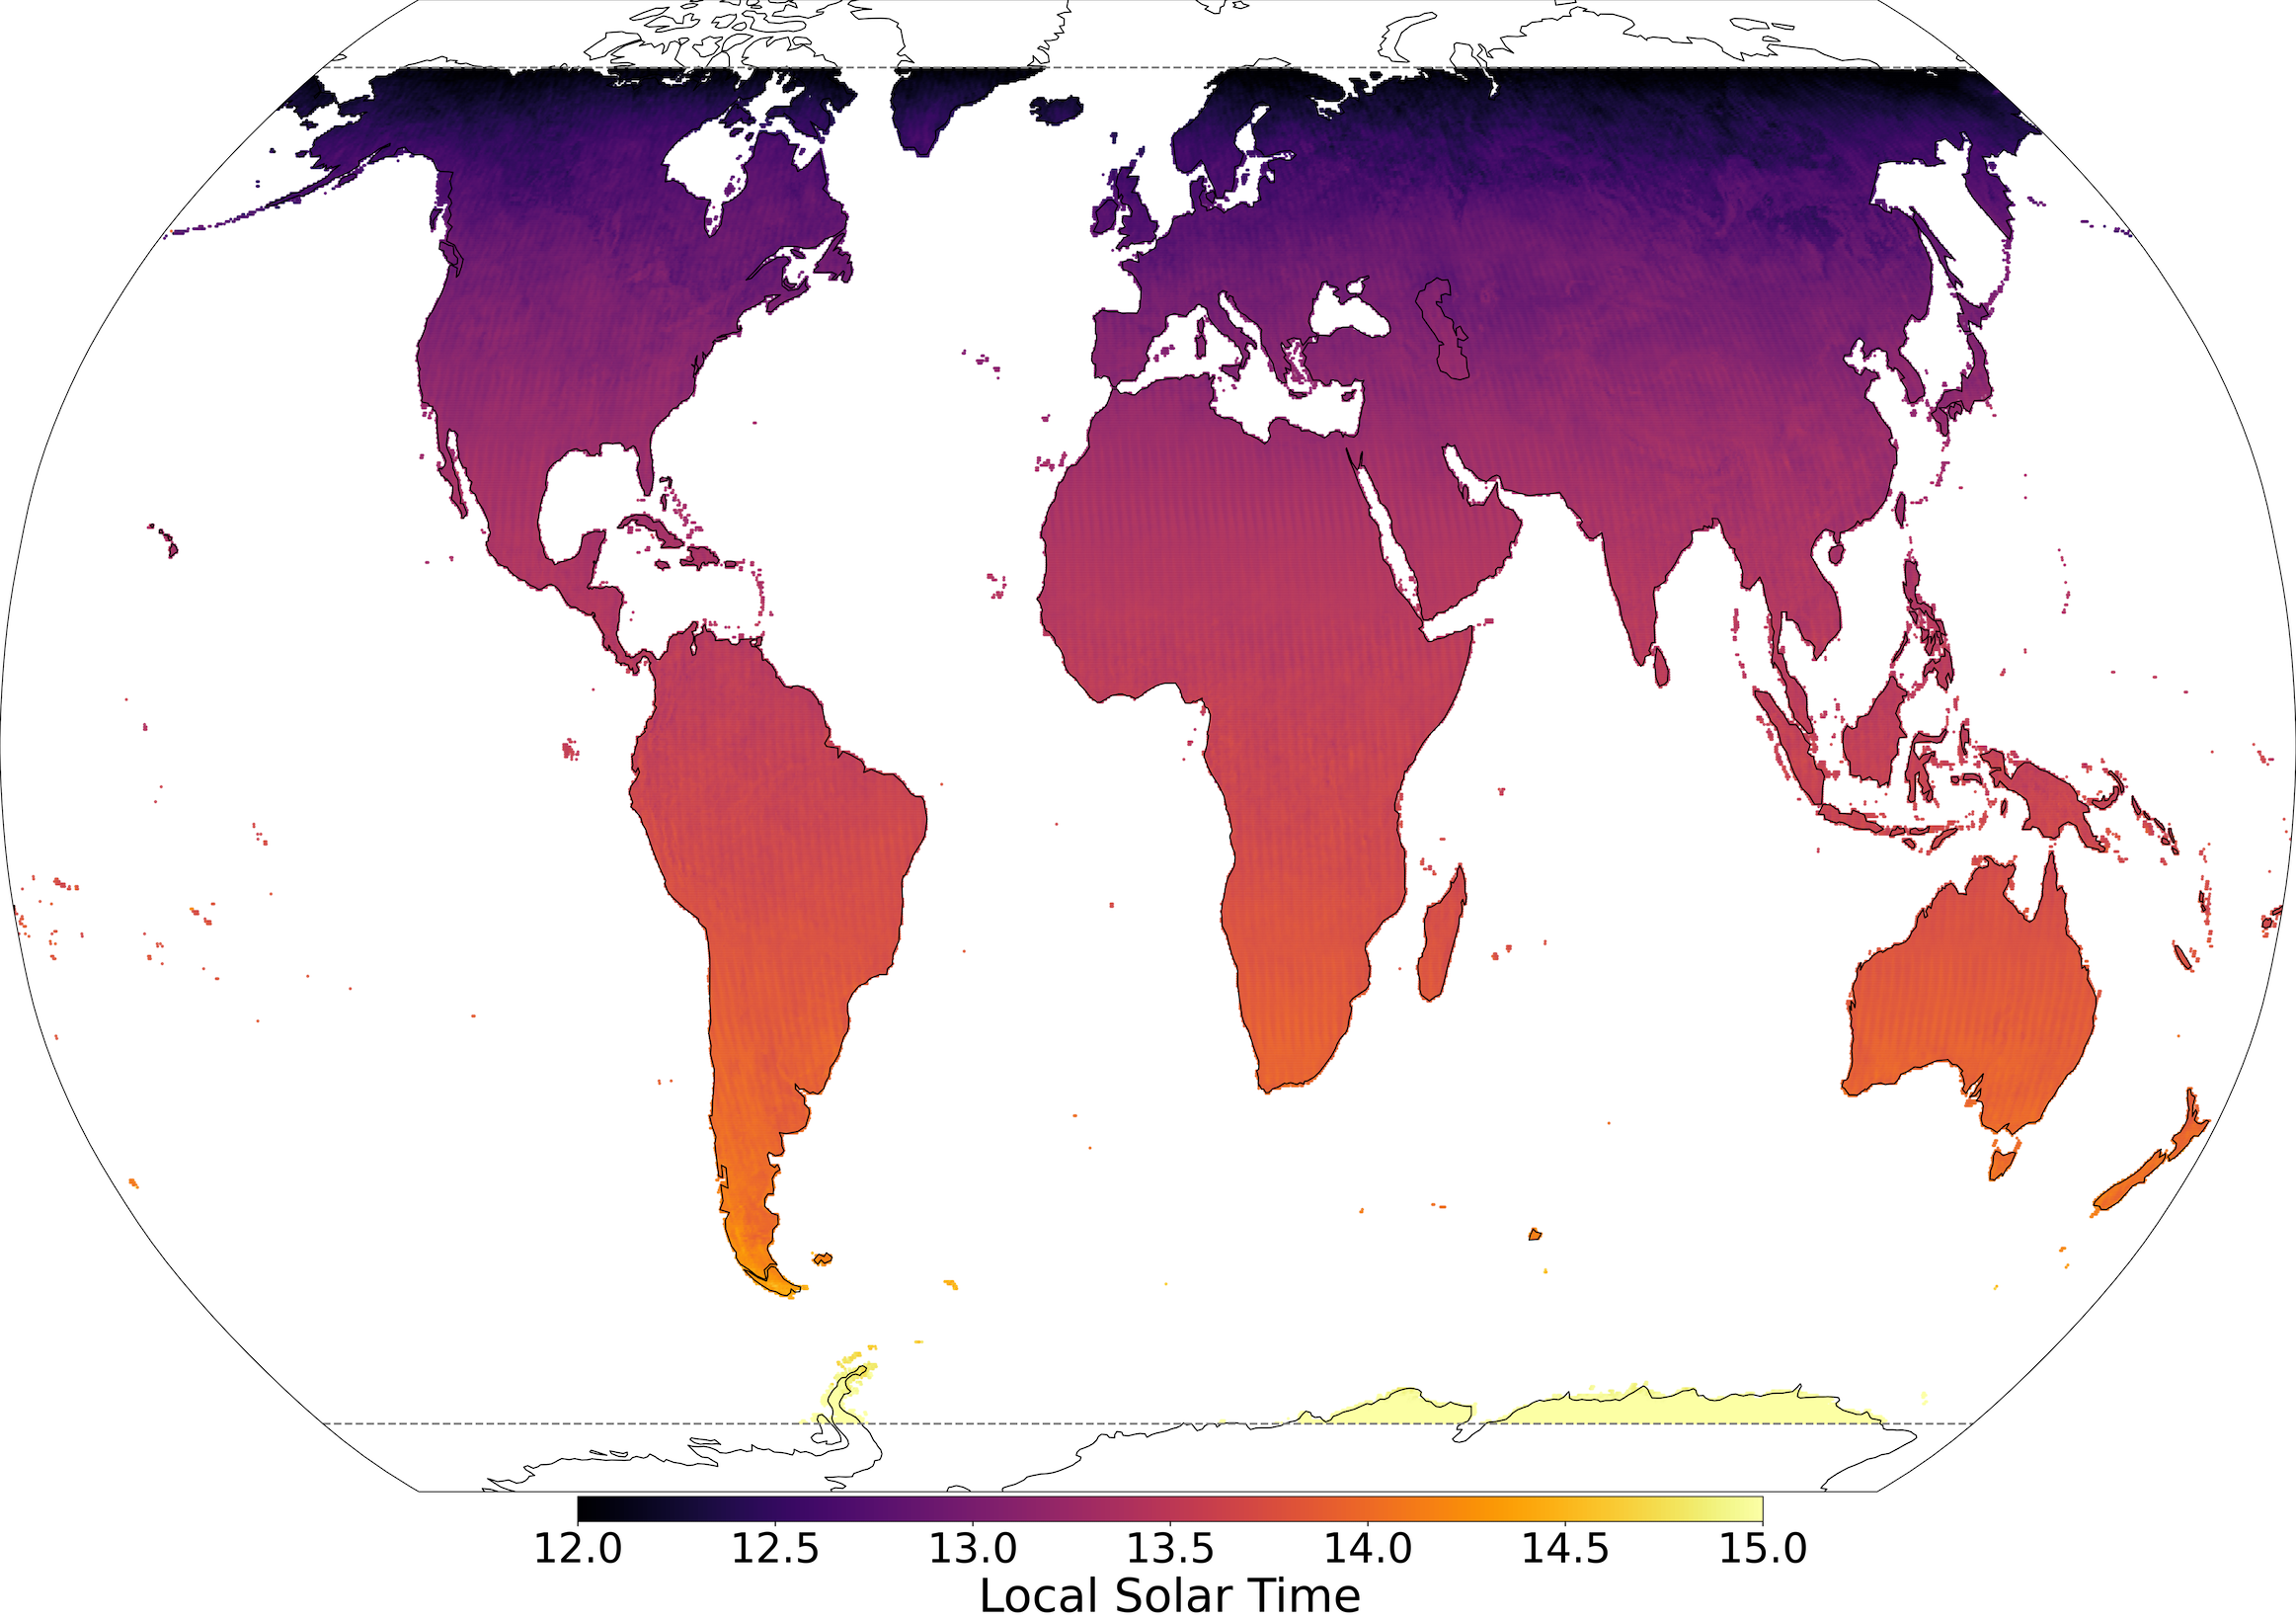
\includegraphics[width=0.48\textwidth]{MODIS_local_solar_time}} \\
	\subfloat[\label{fig:Modistime1}]{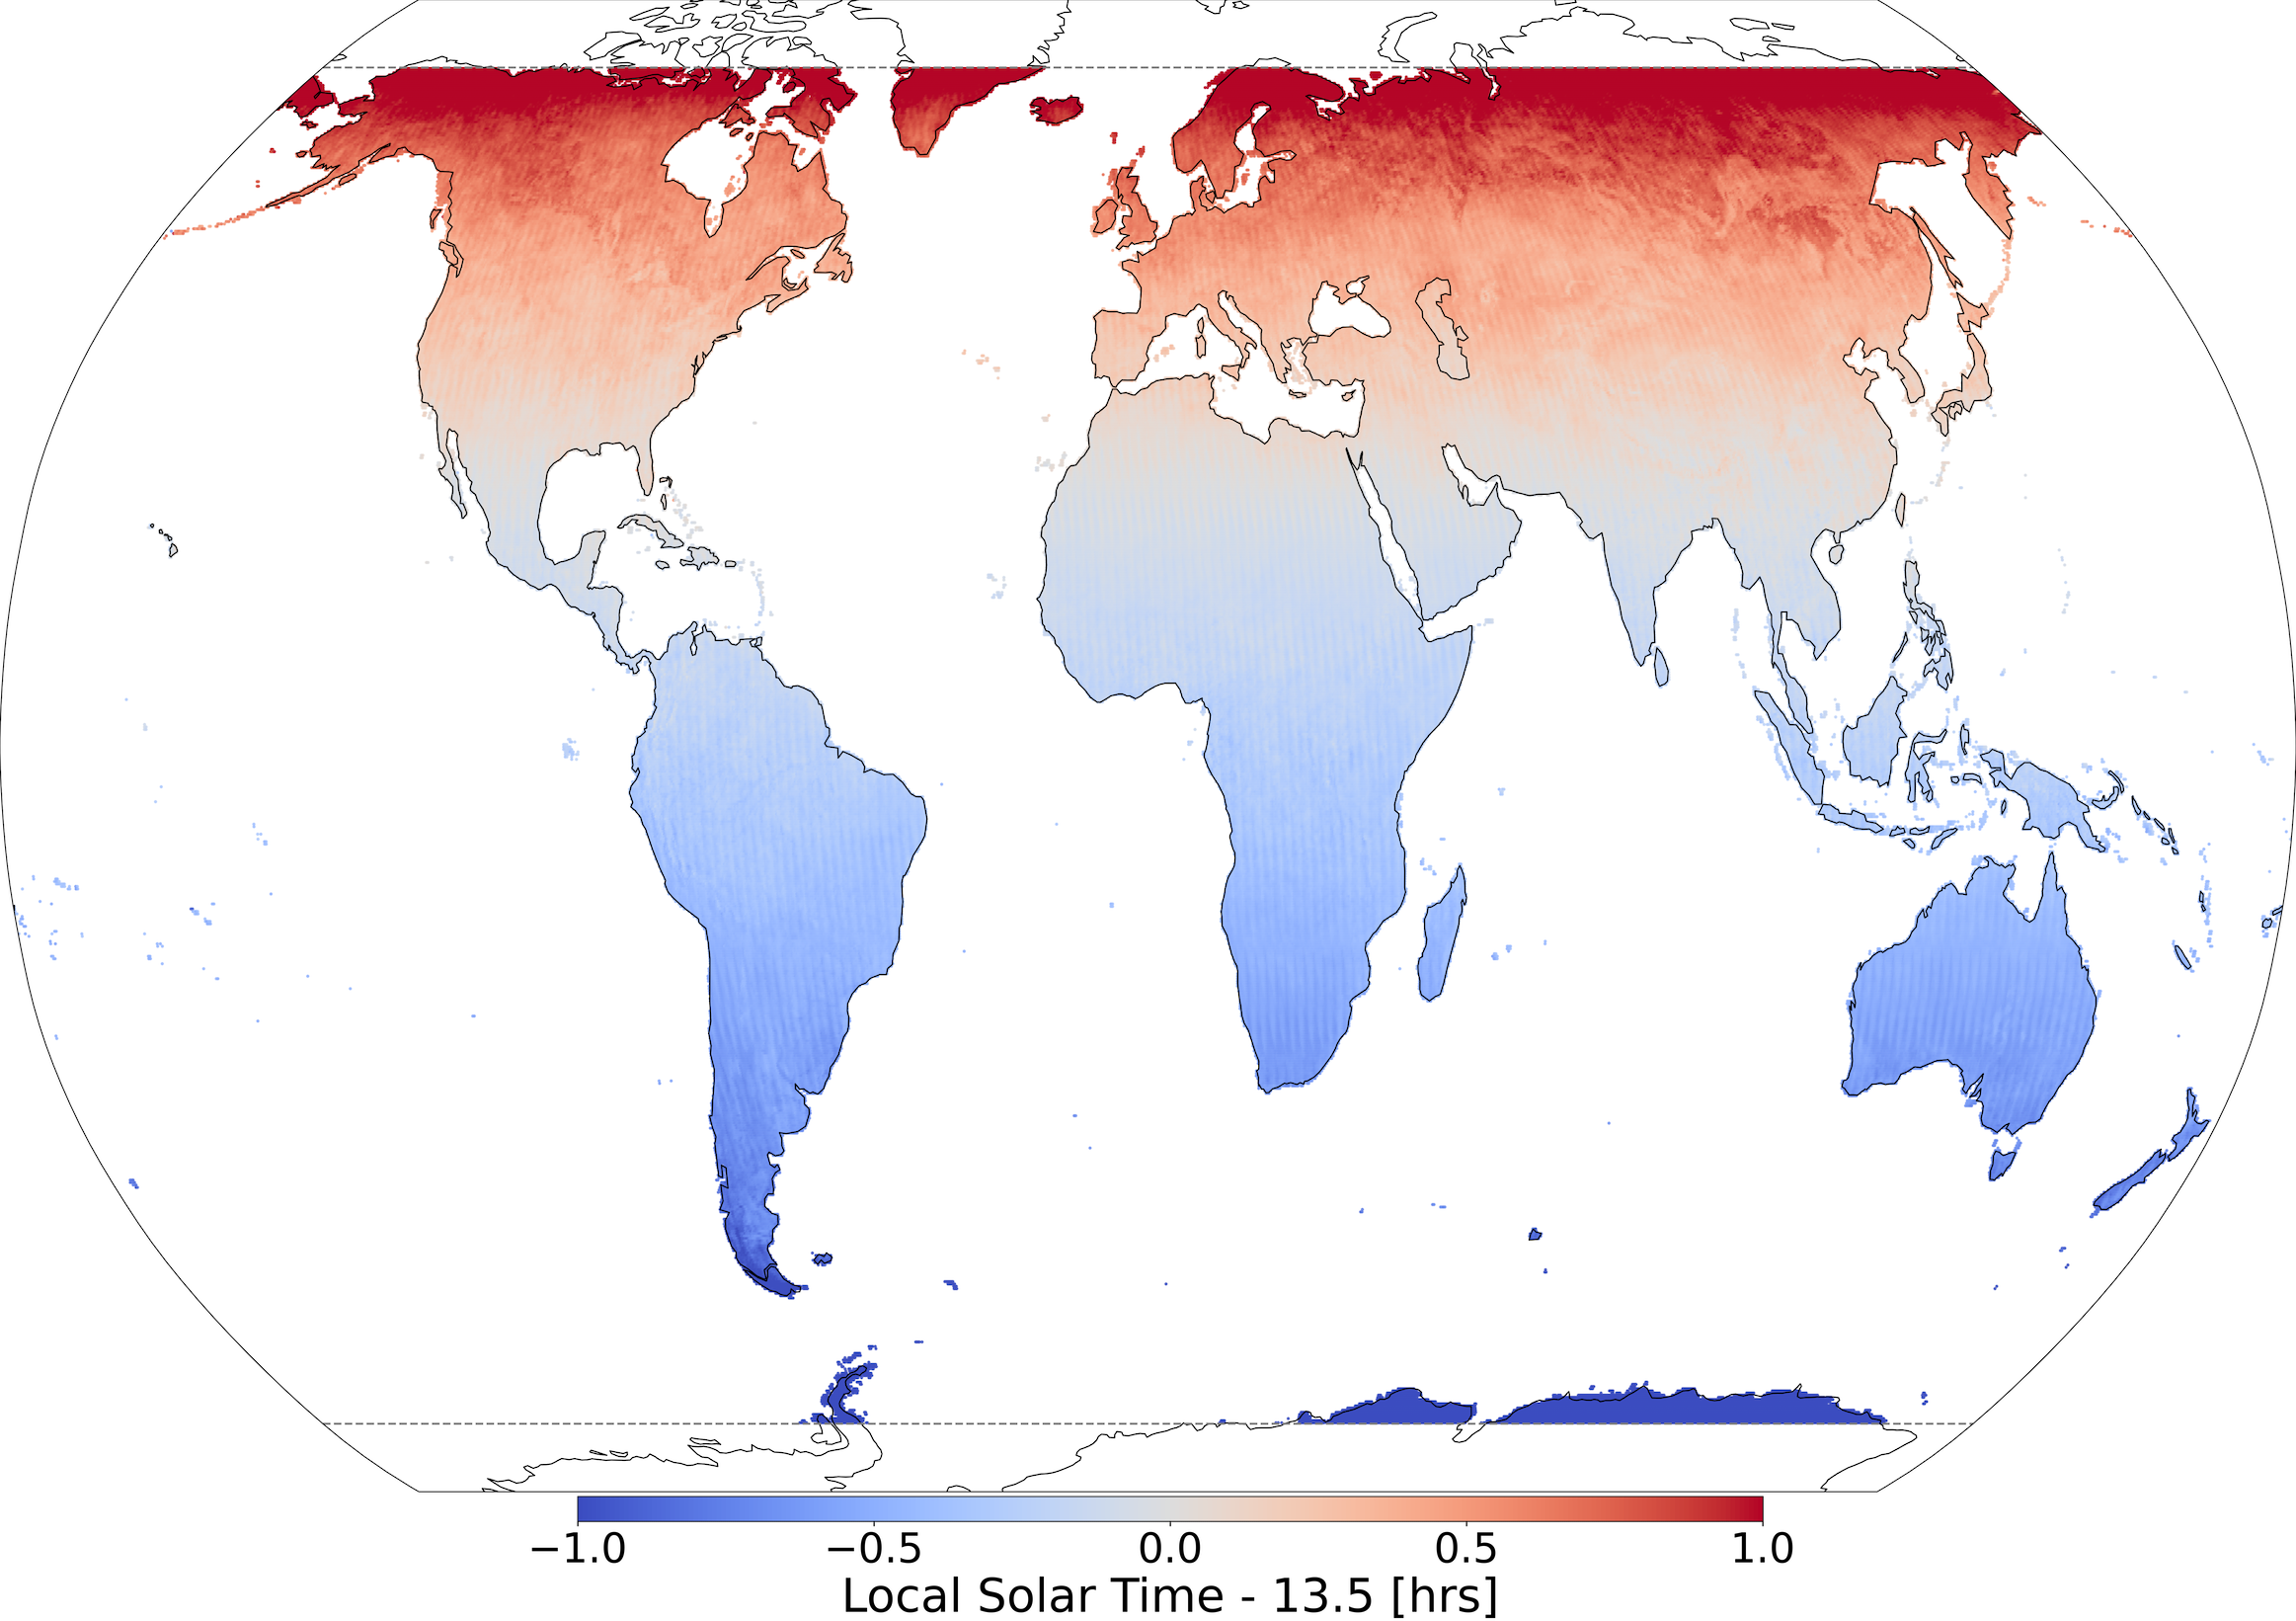
\includegraphics[width=0.48\textwidth]{MODIS_local_solar_time_diff}}
	\caption{Average \textit{(a)} Local solar time of MODIS Aqua day, \textit{(b)} Error relative to the assumed local solar time of 13.30 for the year 2019 at a 31km resolution. The errors are generally sub-hr and grow at greater latitudes. We exclude data with latitudes $|\theta| < 70^{\circ}$ and take 13.30 as a constant local solar time.} 
	\label{fig:MODIS_time}
\end{figure}

\begin{figure}
	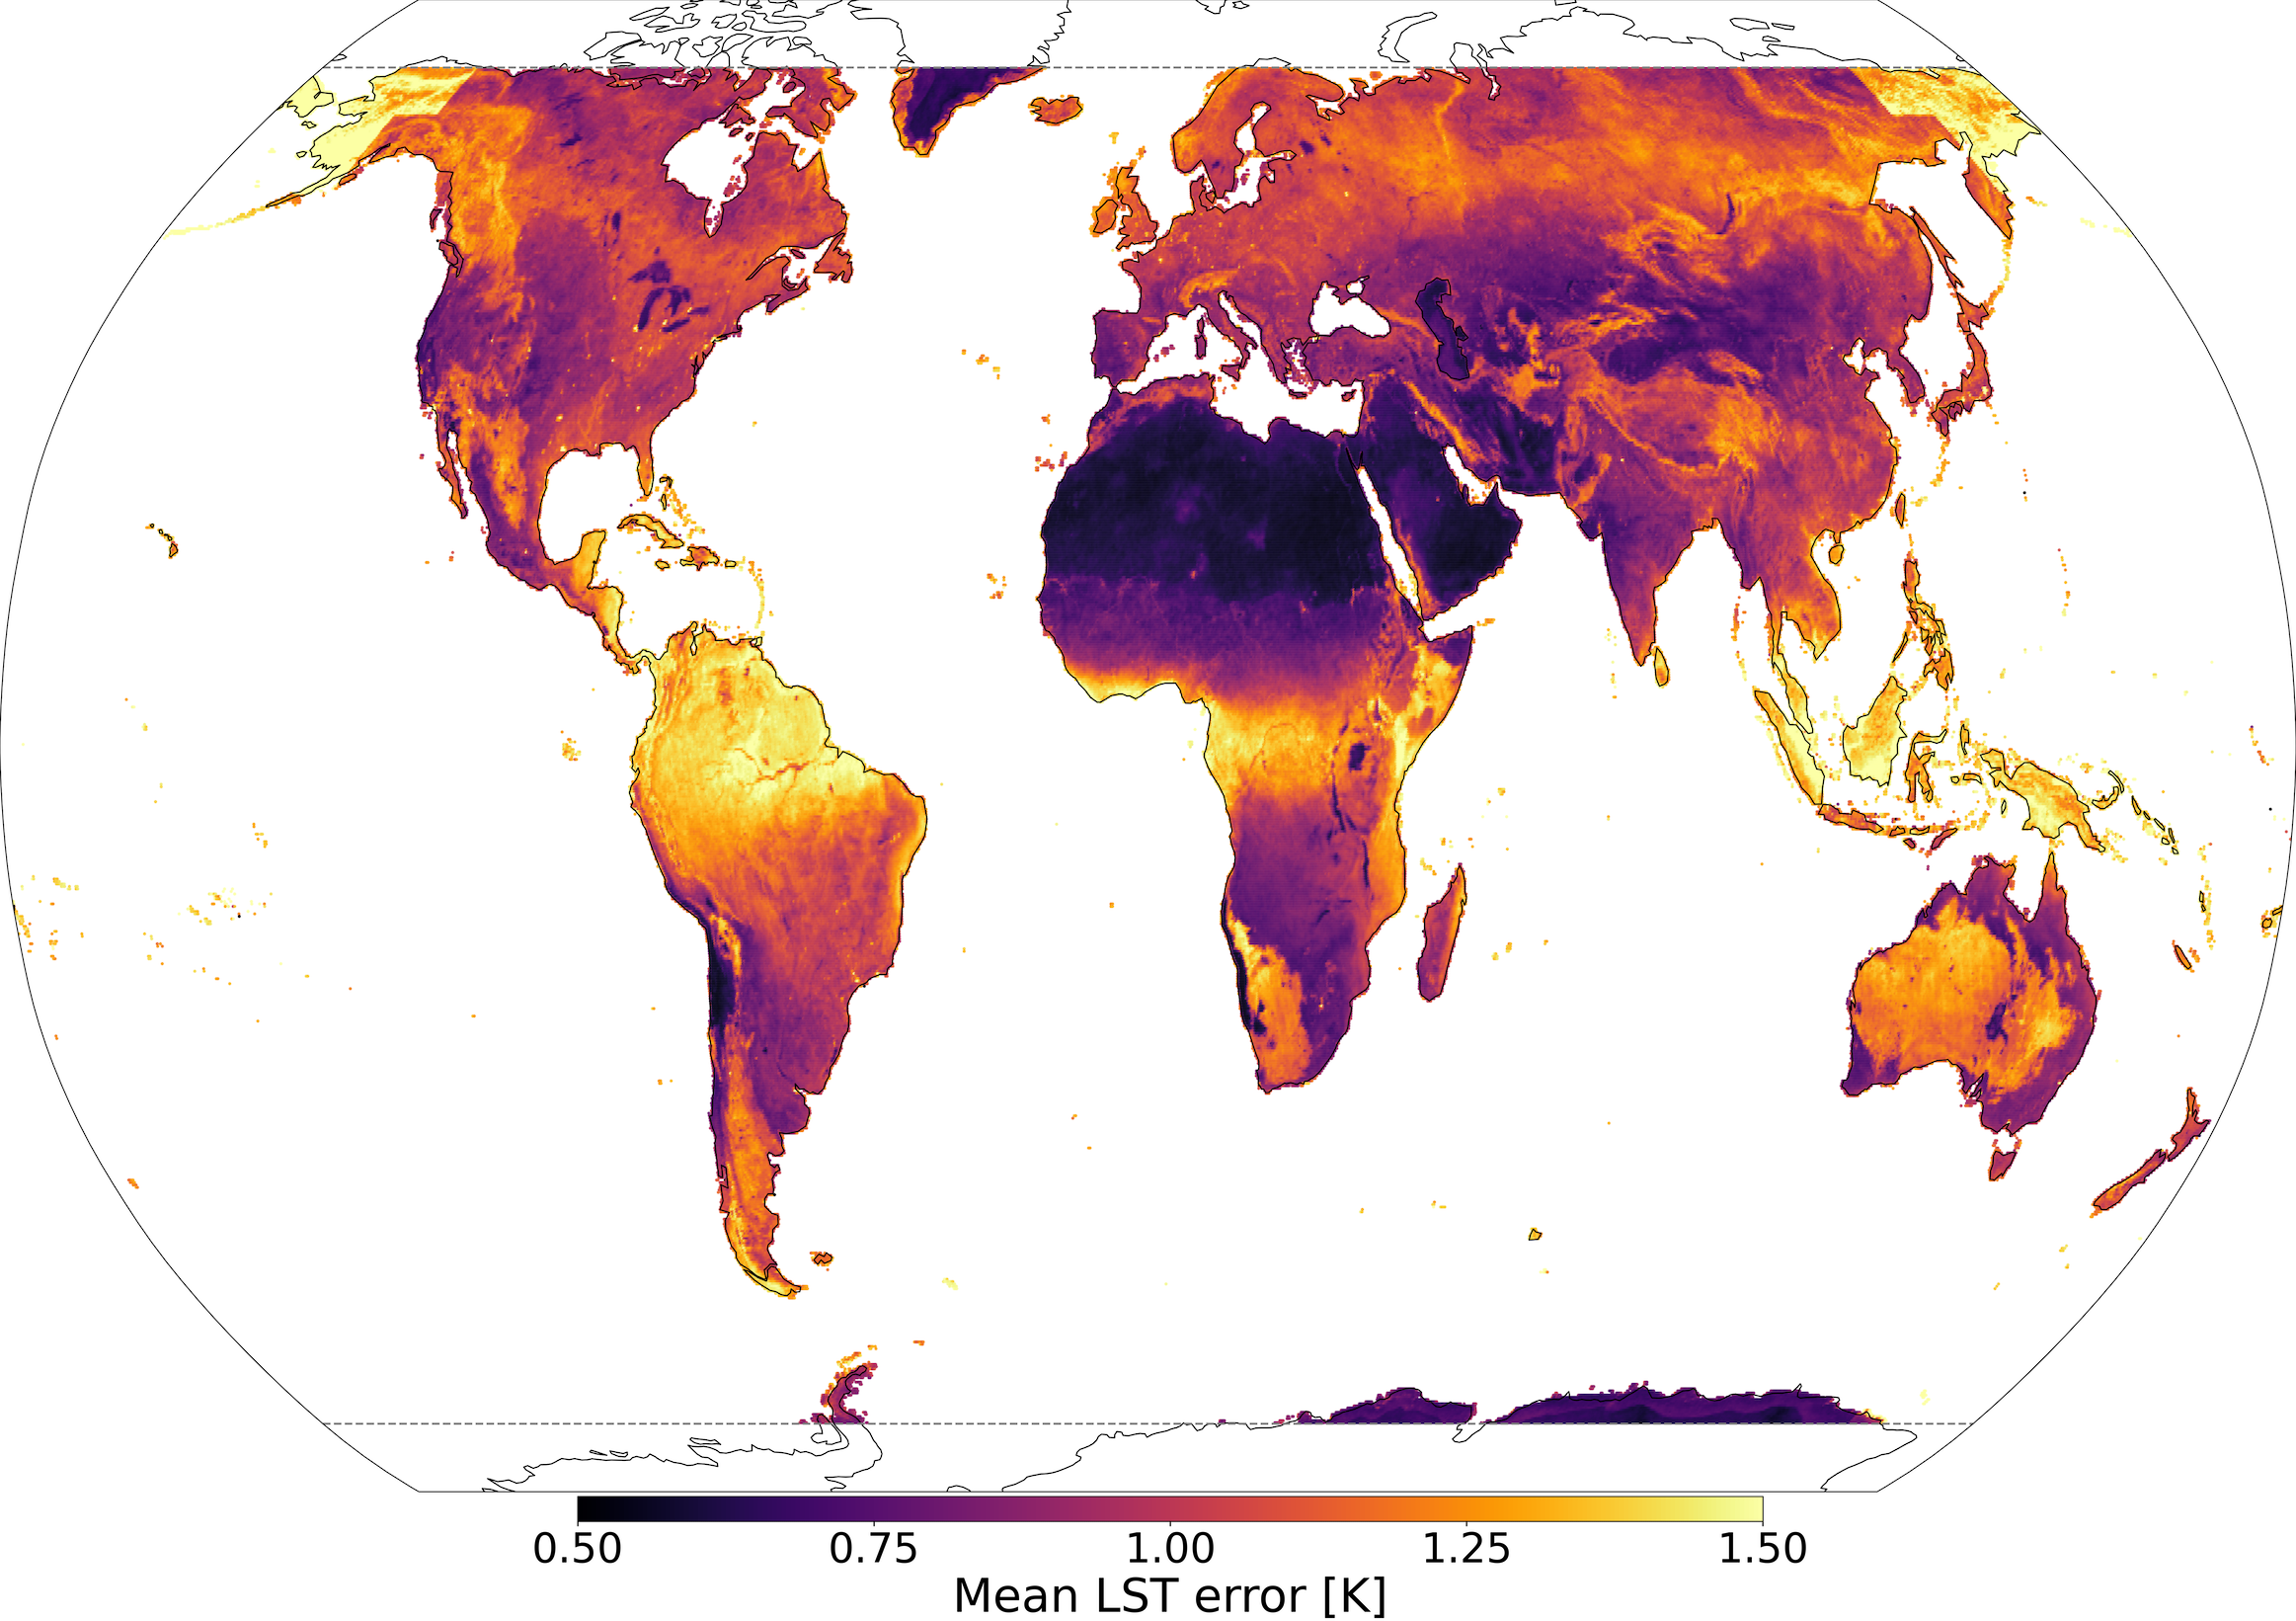
\includegraphics[width=0.48\textwidth]{MODIS_obs_error}
	\caption{Average error in the MODIS LST measurement at a 31km resolution. The raw MODIS data at a 1km resolution provides categorical LST errors with bins $\leq 1$K, $1 - 2$K $2-3$K and $>3$K. When averaging to 31km resolution we compute a weighted average over the 1km grid cells, where we take the median bin value, and $5$K for the $>3$K bin.} 
	\label{fig:MODIS_obs_error}
\end{figure}

\noindent With the MODIS data converted to an hourly UTC it is then straightforward to match this to the corresponding hour in the ERA dataset. In order to then match in space we select an hour of data and do the following:
\begin{enumerate}
	\item Take a single MODIS LST observation at a particular point on the MODIS grid.
	\item Find the nearest point on the ERA5 grid to that MODIS grid point.
	\item Repeat for every MODIS observation
	\item Group by the ERA5 grid points, averaging over all the MODIS observations that are associated with each ERA5 point. 
\end{enumerate}
The result of this process is then for every set of ERA5 input fields at a particular point in space and time, we have an empirical LST ``observation" which is an average over $n$ MODIS observations (see e.g. Fig \ref{fig:MODIS_obs}). We take this averaged observation as the ground truth $y$ that we are trying to predict in our regression model.  Step 2 in the joining pipeline  uses a GPU-accelerated k-nearest neighbours algorithm\cite{Rapids}, where ``nearness" is measured via the Haversine metric i.e.  the geodesic distance on the sphere between two points: 
\begin{equation}
	H = 2 \arcsin (d)
\end{equation}
where
\begin{eqnarray}
	d = \sqrt{\sin^2\left(\frac{\delta\theta}{2}\right) + \cos \theta_1 \cos \theta_2 \sin^2\left(\frac{\delta \phi}{2}\right) }
\end{eqnarray} 
for two points with coordinate latitudes $\theta_{1,2}$, longitudes $\phi_{1,2}$ and $\delta \theta = \theta_2 - \theta_1$ and  $\delta \phi = \phi_2 - \phi_1$ . 
\begin{figure}
	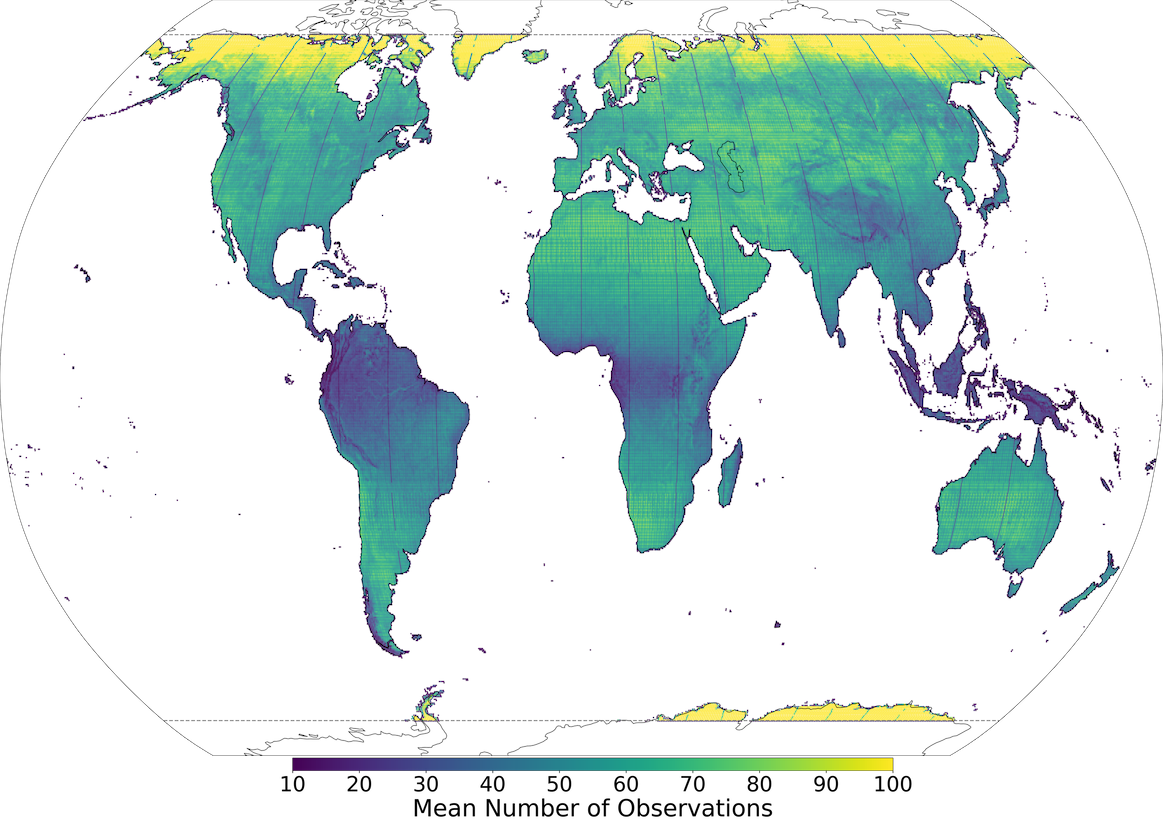
\includegraphics[width=0.48\textwidth]{num_obs_map.png}
	\caption{Mean daily number of MODIS observations mapped to each ERA5 data point for 2019. The swath of the Aqua satellite is clearly visible, with more observations at more extreme latitudes as Aqua follows a polar orbit, south to north. In addition to the expected increased sparsity of observations at the equator, there are also notably fewer observations in regions of greater orography such as the Himalayas, the Andes and the  Rocky Mountains as well as the Siberian Tundra, due to increased cloud cover.} 
	\label{fig:MODIS_obs}
\end{figure}

\subsection{Constructing a regression model}
We have our features $\bar{x}$ and target $y$ data in a related format. We are now in a position to train a regression model to learn the mapping between $\bar{x}$ and $y$. For this purpose we use a sequential neural network architecture, implemented on Tensorflow\cite{tensorflow2015-whitepaper}. Whilst more advanced architectures and regression models are available, for our purposes the sequential model is more than sufficient and it exhibits generally fast and dependable convergence. We take as our canonical structure a network where the number of nodes in the input layer is equal to the number of training features, a single node in the output layer corresponding to the LST and 4 hidden layers where the number of nodes in each layer is equal to the half the number of input nodes.  For our optimisation scheme we use ADAM\cite{2014adam} and set the learning rate to $3 \times 10^{-4}$, and the exponential decay rate for the 1st and 2nd moment estimates take default values of $0.90$ and $0.999$. The network is not trained for a fixed number of epochs, but instead trained until the validation error reaches a minimum. Techniques for maximising the performance of a network via hyperparameter optimisation are now well established\cite{HPO1,HPO2}. However for our purposes we do not try in any meaningful way to tune our hyperparameters, instead just take some reasonable default values which we judge to be ``good enough''. Some shallow exploration of different hyperparameter configuration was undertaken, but for this data the prediction accuracy is mostly independent of the hyperparameter configuration, subject to standard and reasonable hyperparameter choices. Whilst a more advanced automatic hyperparameter optimization method may have enabled slightly more performance to be squeezed out of the model, our ultimate purpose is not to generate the most absolutely accurate prediction possible, but instead to have two predictive models which we can compare. Additionally, as we will see, the variation in performance due to modifications to the input features is far greater than the variation due to the hyperparameter choices. \newline 

\noindent With a fully trained network we can then deploy the model to make predictions of the LST over the whole globe. An example of the error in the predicted LST relative to the true MODIS LST, is presented  in Figure \ref{fig:example_model}. The model was trained on a year of ERA5 data from 2016 and then made predictions of the LST in 2019. We can compare the error in the model predictions with the error in the predicted skin temperature that is derived from ERA5. It is evident from Figure \ref{fig:example_model} that the trained model generally enjoys increased accuracy over the ERA5 predictions, especially in the Himalayas and sub-Saharan Africa as well as Australia and the Amazon basin. For this particular example, the mean annual error, averaged over all grid points was 3.9 K for the ERA5 prediction and 3.0 K for the model prediction. This serves as a useful sanity check to give us confidence that the network is performing as expected and gives generally reasonable predictive performance, at least as good - if not better - than then derived skin temperature predictions from ERA5. More fundamentally, this also indicates that there is some information captured in the input fields to the network that is not expressed through the current ERA5 reanalysis modelling. This again motivates the development of updated parametrization schemes that better represent small scale processes and better capture this information.  \newline

\begin{figure*}
	\subfloat[\label{fig:wasserstein_temperature}]{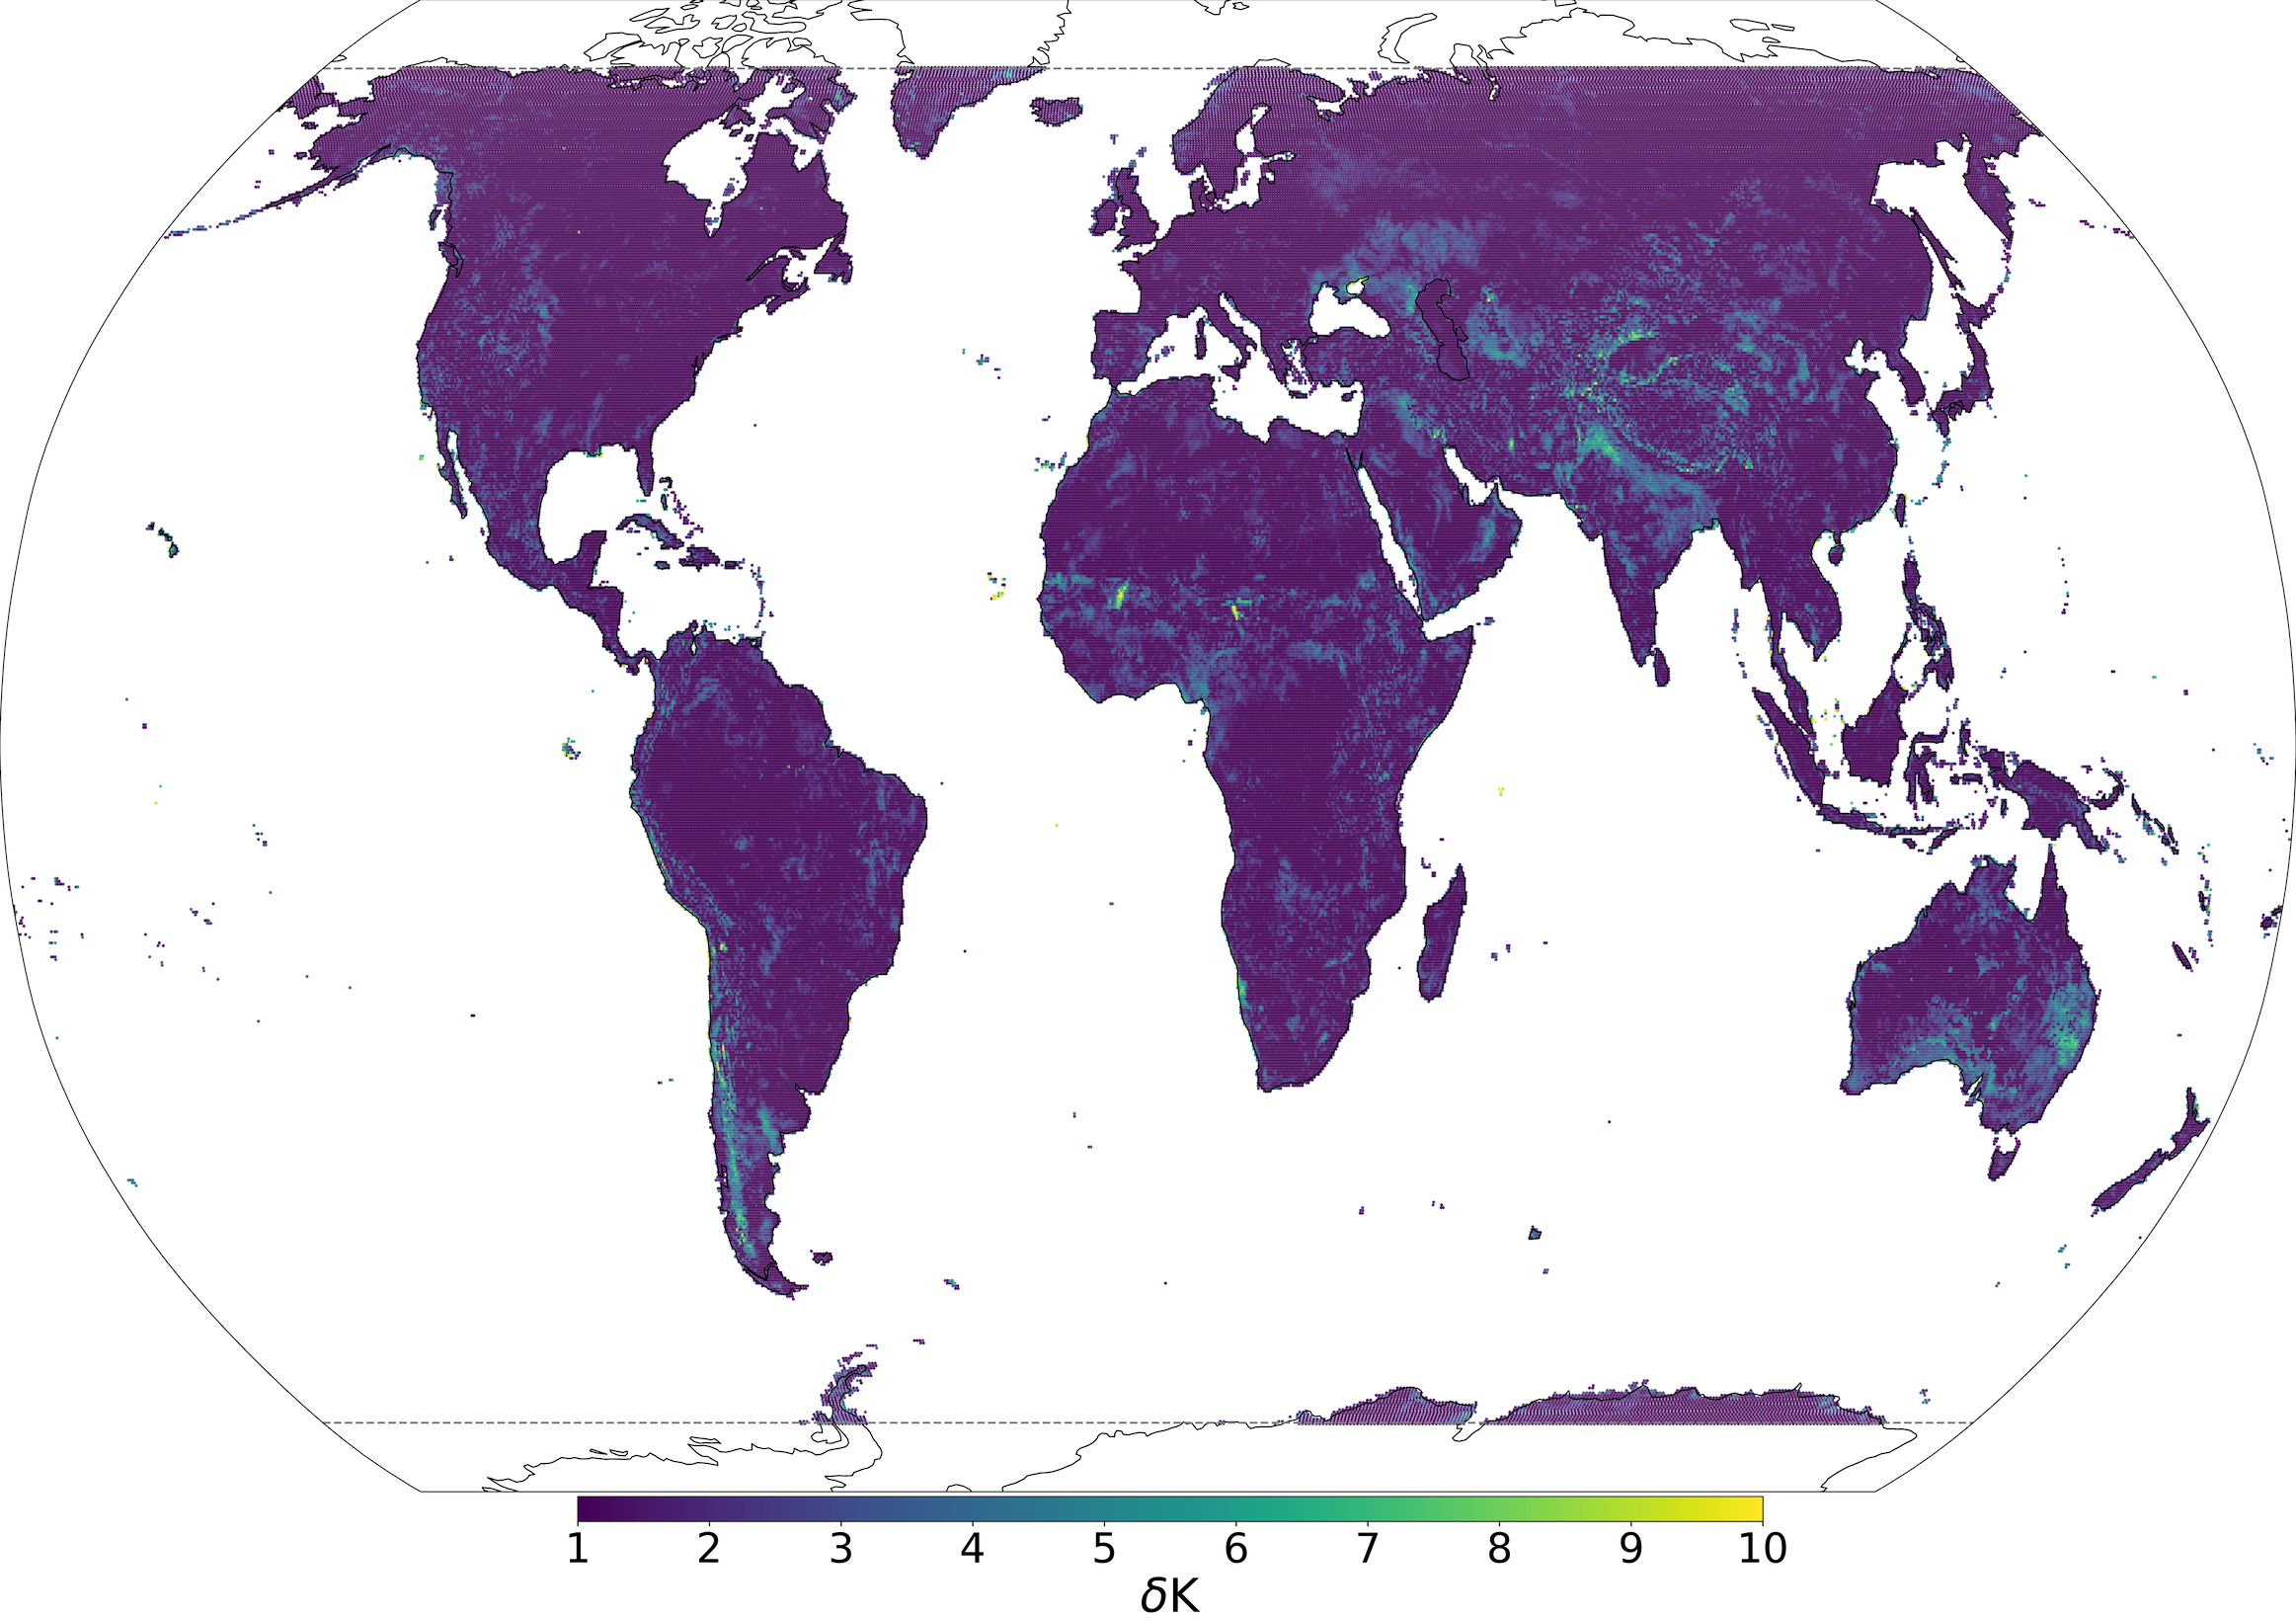
\includegraphics[width=0.48\textwidth]{model_prediction_error.png}} \hspace{1mm}
	\subfloat[\label{fig:wasserstein_precipitation}]{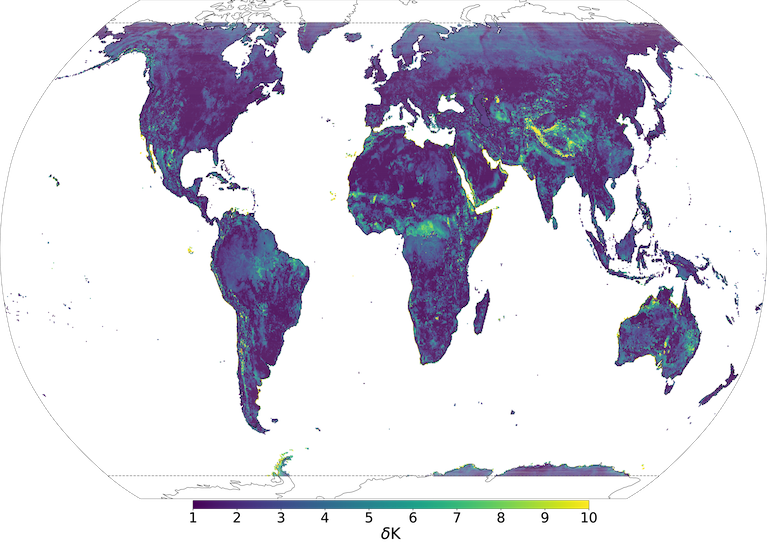
\includegraphics[width=0.48\textwidth]{ERA_prediction_error.png}}
	\caption{Prediction error relative to MODIS Aqua observations in the land surface temperature  ($\delta K$) for 2019, averaged over the year, for \textit{(a)} Trained Neural Network and \textit{(b) }ERA5. It can be seen that the network generally outperforms the ERA5 predictions, which generally struggles in regions with complex surface fields such as the Himalayas (lots of orography) sub-Saharan Africa (lots of vegetation) and the Amazon Basin (lots of water + vegetation). In contrast the network demonstrates generally good performance, with some drop off in the Himalayas and the eastern cost of Australia, but still outperforming ERA5.} 
	\label{fig:example_model}
\end{figure*}



\section{Evaluating Updated Lake Fields}\label{sec:3}
As discussed, at ECMWF parametrised lake representation in the IFS is handled by FLake.The primary physiographic dataset used in the IFS to generate the lake parameters is the GlobCover2009 global map  \cite{GLOBCOVER}\cite{arino2012glcm}. This map has a resolution of 300m and covers latitudes from $60^{\circ}$S to $85^{\circ}$N; corrections outside this latitude band for the polar regions and Iceland are included separately.  In the Arctic no land is assumed, whilst in the Antarctic data from version 2 of the Radarsat Antarctic Mapping Project (RAMP2) digital elevation model (DEM) is used\cite{Liu2015}. For Iceland, data from the Digital map database of Iceland (IS 50V) is used. \newline 


\noindent More recently, new datasets and methods for updating the lake fields for the IFS have been proposed\cite{Choulga2019}. These new datasets include the Global Surface Water Explorer (GSWE) dataset from the Joint Research centre (JRC) \cite{GSWE}. GSWE is a 30m resolution dataset from Landsat 5,7 and 8, providing  information on the spatial and temporal variability of surface water on the Earth since March 1984. This then allowed for particular geographical regions to be updated with more up-to-date, high resolution data, providing additional information that is not captured by GlobCover2009. Whilst multiple lake areas were updated based on this new data, particularly noteworthy regions include:
\begin{itemize}
	\item \textbf{Aral Sea}. The Aral Sea lies across the border between Uzbekistan and Kazakhstan and was at one point the 4th largest lake in the world. However, the Aral Sea has long been shrinking, at an accelerated rate since the 1960s. It started to stabilise in 2014 with an area of $7660 \text{km}^2$, 9 times smaller than its size in 1960, and its eastern basin is now known as the Aralkum Desert. The water map from GlobCover2009 describes the Aral Sea in 1998, when it was still ``only" 2 times smaller than its 1960 extent, whereas GSWE provides a more up to date map.
	\item \textbf{Australia}. GlobCover2009 over-represents inland water in Australia, which generally has a huge number of lakes. However, some of these lakes are highly ephemeral;  the endorheic Kati Thanda–Lake Eyre fills only a few times per century. The GSWE updates to this region therefore include only generally permanent water, removing all seasonal and rare ephemeral water. 
\end{itemize} 
The lake depth is not specified by GlobCover2009/GSWE, instead being described by the Global Lake DataBase (GLDB) \cite{Kourzeneva2012}. Lake depth is recognized as being an important field in the IFS, since over estimates can result in strong cold biases in hotter seasons or else a lack of ice formation. Under the program to continuously update the parametrisation schemes, recently the original version of the dataset, GLDBv1,with coarse resolution aggregation technique MEAN, has been superseded by GLDBv3\cite{Choulga2014}, with coarse resolution aggregation technique MODE. GLDBv3 increases the total number of lakes with in situ information by $\sim1500$, introduces a depth distinction between freshwater and saline lakes, and updates the method by which the lake depth is calculated based on climate type and geological origins. Consequently, whilst the updated fields when going from GlobCover2009 to GSWE applied at particular geographic regions, the lake depth field is generally updated globally. Verification of the updated lake depth fields against 353 lakes in Finland shows that GLDBv3 exhibits a 52$\%$ bias reduction compared to GLDBv1\cite{Choulga2019}. For a thorough discussion of the upgraded lake fields, the lake depth, and the representation of lakes generally by ECMWF we refer the reader to\cite{Choulga2019,Boussetta2021}. \newline 

\noindent This distinction between the original lake maps based on GlobCover2009 and GLDBv1 data and the updated lake maps which have been corrected using GSWE and GLDBv3 data provides an ideal test bed to deploy and demonstrate our tool. Can we use VESPER to evaluate the added value of these new fields? 

\subsection{V15 vs V20}
In order to ascertain the accuracy and information content of the updated lake fields we will proceed as follows. We will train two permutations of the regression model, one where the ERA5 input features are based on data from the original GlobCover2009/GLDBv1 data maps, and a second which has these original features, plus additional corrections from the GSWE/GLDBv3 datasets. Each feature which is derived from the original datasets has a corresponding updated correction based on the new datasets. For instance, in the first model there is an input feature for the lake depth, and in the second model there is the lake depth feature plus a ``lake depth correction feature". As a shorthand we will refer to a network model with the original fields based on GlobCover2009 maps as ``V15'' (FLake was first introduced in 2015) and a model which also includes updated fields based on the GSWE corrections as ``V20". All non-lake related climate fields such as vegetation or orography were updated in V20 only in relation to the changing lake fields (e.g. if the grid box lake fraction increased, the vegetation fraction decreased accordingly). Additionally, both permutations of the model share a set of time variable-fields which are not updated by the lake model, such as the 2m-temperature or the wind components, etc. To summarise:
\begin{enumerate}
	\item \textbf{V15 Model Features}: Time variable fields + original time constant fields based on GlobCover2009/GLDBv1 data.
	\item \textbf{V20 Model Features}: Time variable fields + original time constant fields based on GlobCover2009/GLDBv1 data + time constant field corrections from GSWE/GLDBv3 data.
\end{enumerate}
The full list of features used is presented in Table \ref{tab:1}. 
\begin{table*}[t]
	\centering
	\begin{tabular}{llc}
		Feature              & Physical Meaning & Updated in V20?  \\
		\hline
		sp & Surface pressure &  \\
		msl & Mean sea level pressure &  \\
		u10 & 10 metre u-wind component &  \\
		v10 & 10 metre v-wind component &  \\
		t2m & 2 metre temperature &  \\
		d2m & 2 metre dewpoint temperature  &  \\
		skt & Skin temperature &  \\
		istl1 & Ice temperature layer 1 &  \\
		istl2 & Ice temperature layer 2 &  \\
		aluvp & UV visible albedo for direct radiation &  \\
		aluvd & UV visible albedo for diffuse radiation &  \\
		alnip & Near IR albedo for direct radiation &  \\
		alnid & Near IR albedo for diffuse radiation &  \\
		fal & Forecast albedo &  \\
		sd & Snow depth &  \\
		sdfor & Standard deviation of filtered subgrid orography &  \checkmark \\
		sdor & Standard deviation of orography &  \checkmark \\
		isor & Anisotropy of sub-gridscale orography &  \checkmark \\
		anor & Angle of sub-gridscale orography & \checkmark  \\
		slor & Slope of sub-gridscale orography &  \checkmark \\
		z & Geopotential &  \checkmark \\          
		lsm & Land-sea mask (fractional) &  \checkmark \\   
		si10 & Glacier cover &  \checkmark \\               
		cl & Lake cover &   \checkmark \\
		dl & Lake mean depth & \checkmark  \\        
		cvl & Low vegetation cover &   \checkmark\\
		cvh & How vegetation cover &   \checkmark\\
		tvl & Low vegetation dominant type&   \checkmark\\
		tvh & High vegetation  dominant type&  \checkmark \\
		slt & Soil type & \checkmark  \\
		
		
		\hline
	\end{tabular}
	\caption{Input features used for training the model, along with information on whether the fields were updated when going from the original data based on GlobeCover2009/GLDBv1 to GSWE/GLDBv3. All the fields which were updated are static fields, whilst all those that were not updated are time-variable fields.}
	\label{tab:1}
\end{table*}
\noindent By comparing the accuracy of the predictions of the two models we can then discern the value gained from updating these static surface fields. \newline 


\noindent There is an inherent noise in the regression model due to the stochasticity of the network; training the model twice with the same architecture, inputs and parameters can find two different minima. Moreover, for the majority of the globe the lake fields have not been updated, since there are no lakes there! By inspecting the predictions at a grid point where the fields have not been updated in going from V15 to V20 we obviously don't learn anything, instead just measuring the intrinsic model noise, i.e. the different optimisation minima discovered by the model. By comparing two models with the same network structure, trained on the same data, we estimate the noise bias to be 0.04 K over all grid points. Instead we want to restrict our analysis to areas where there have been a significant changes in the fields. More quantitively, we consider a ``significant change" to be a change in the surface field when going from V15 to V20 of $\geq 0.1 $ for fractional fields of  $\geq 10 \%$ for non-fractional quantities. So for example, if the field for the lake cover (\textit{cl}) - which describes the fraction of the grid box which is classified as a lake - changes from 0.1 in V15 to 0.3 in V20 this would be classified as a significant change. Similarly, if the lake depth - a non fractional quantity - changes from 10m to 20m, this would also be a significant change. Naturally the choice of $\geq 10 \%$ is a somewhat arbitrary tolerance cut-off, but it balances the trade off between having a sufficient number of grid points to inspect and the strength of the effect of changing the input field. As the tolerance increases we isolate points where the fields have been changed more severely, but have fewer points, whereas when the tolerance decreases we have more points but it is more difficult to disentangle the change in the prediction accuracy from the model noise. Alternative tolerances were briefly explored, but our conclusions are broadly unchanged. \newline 


\noindent Grid points can be classified according to how the surface fields are updated when going from V15 to V20. We will examine 3 illustrative categories:
\begin{itemize}
	\item \textbf{Lake Updates}. The change in the lake cover \textit{cl} and lake depth \textit{dl} are significant, but the ocean and glacier fractions are not. This corresponds to grid boxes where inland lakes have been added or removed. We will also use a sub-category \textbf{Lake-Ground Updates} where we have the additional constraint that the change in the high/low vegetation fractions are not significant. This then corresponds to the exchange of lakes for bare ground, or vice versa.
	\item \textbf{Vegetation Updates}. The change in the high vegetation fraction is significant, but the change in lake cover is not significant. This corresponds to grid boxes where large features like forests and woodlands have been updated, exchanged for bare ground or low vegetation.
	\item \textbf{Glacier Updates}. The change in the glacier cover \textit{si10} is significant. This corresponds to any areas where the fraction of glacier ice has been updated.  
\end{itemize}
\noindent These categories are naturally broad, and have no restrictions on all of the other features listed in Table \ref{tab:1}. For instance, changes to the orography will have important influences on temperature through e.g. wind, solar heating etc. Lake depth is similarly important, influencing how a lake freezes, thaws, mixes and its overall dynamical range. We therefore emphasise that these categories do not correspond to grid points where \textit{only} the fields that define the categories have been updated, but instead represent a systematic and consistent update across multiple related fields. \newline 

\noindent We train the model over the entire globe for the year 2016 and make predictions of the land surface temperature for 2019. For each entry in the test set we can determine the prediction accuracy of both the V15 and V20 models. We will use a simple metric $\delta_{\rm M}$ to quantify the difference between an updated model $M$ and the baseline V15 model i.e.
\begin{eqnarray}
	\delta_{\rm M} = M \text{ prediction error} - \text{V15 prediction error} \ .
\end{eqnarray} 
So for example, $\delta_{\rm V20}$ describes the gain of the V20 model relative to the V15 model. A negative $\delta_{\rm V20}$ therefore indicates that the V20 prediction is more accurate, and vice versa. The results for the selected grid point categories are presented in Table \ref{tab:V1520_results}. \newline 


\begin{table*}[t]
	\centering
	\begin{tabular}{llll}
		Category     & Number of grid points         & Mean $\delta_{\rm V20}$ (K) & Mean $\delta_{\rm V20X}$ (K)\\
		\hline
		Lake & 1631 & -0.450 & -0.451\\
		Lake-Ground & 546 & -1.12& -1.09 \\
		Vegetation  & 58 & +0.49 & +0.0048\\
		Glacier & 1057 & -0.14 & -0.24\\
		\hline
	\end{tabular}
	\caption{Mean change in the model prediction accuracy when using the updated fields,  for the selected update categories. The mean $\delta_{\rm M}$ denotes the annual average over all grid points within a category. Negative $\delta_{\rm M}$ values indicate that the addition of the updated fields has improved the prediction, whilst positive $\delta_{\rm M}$ values indicate that the prediction accuracy has degraded, suggesting that erroneous information has been introduced. }
	\label{tab:V1520_results}
\end{table*}






\subsubsection{Category: Lake Updates}\label{V20Lake}
\begin{figure*}[t]
	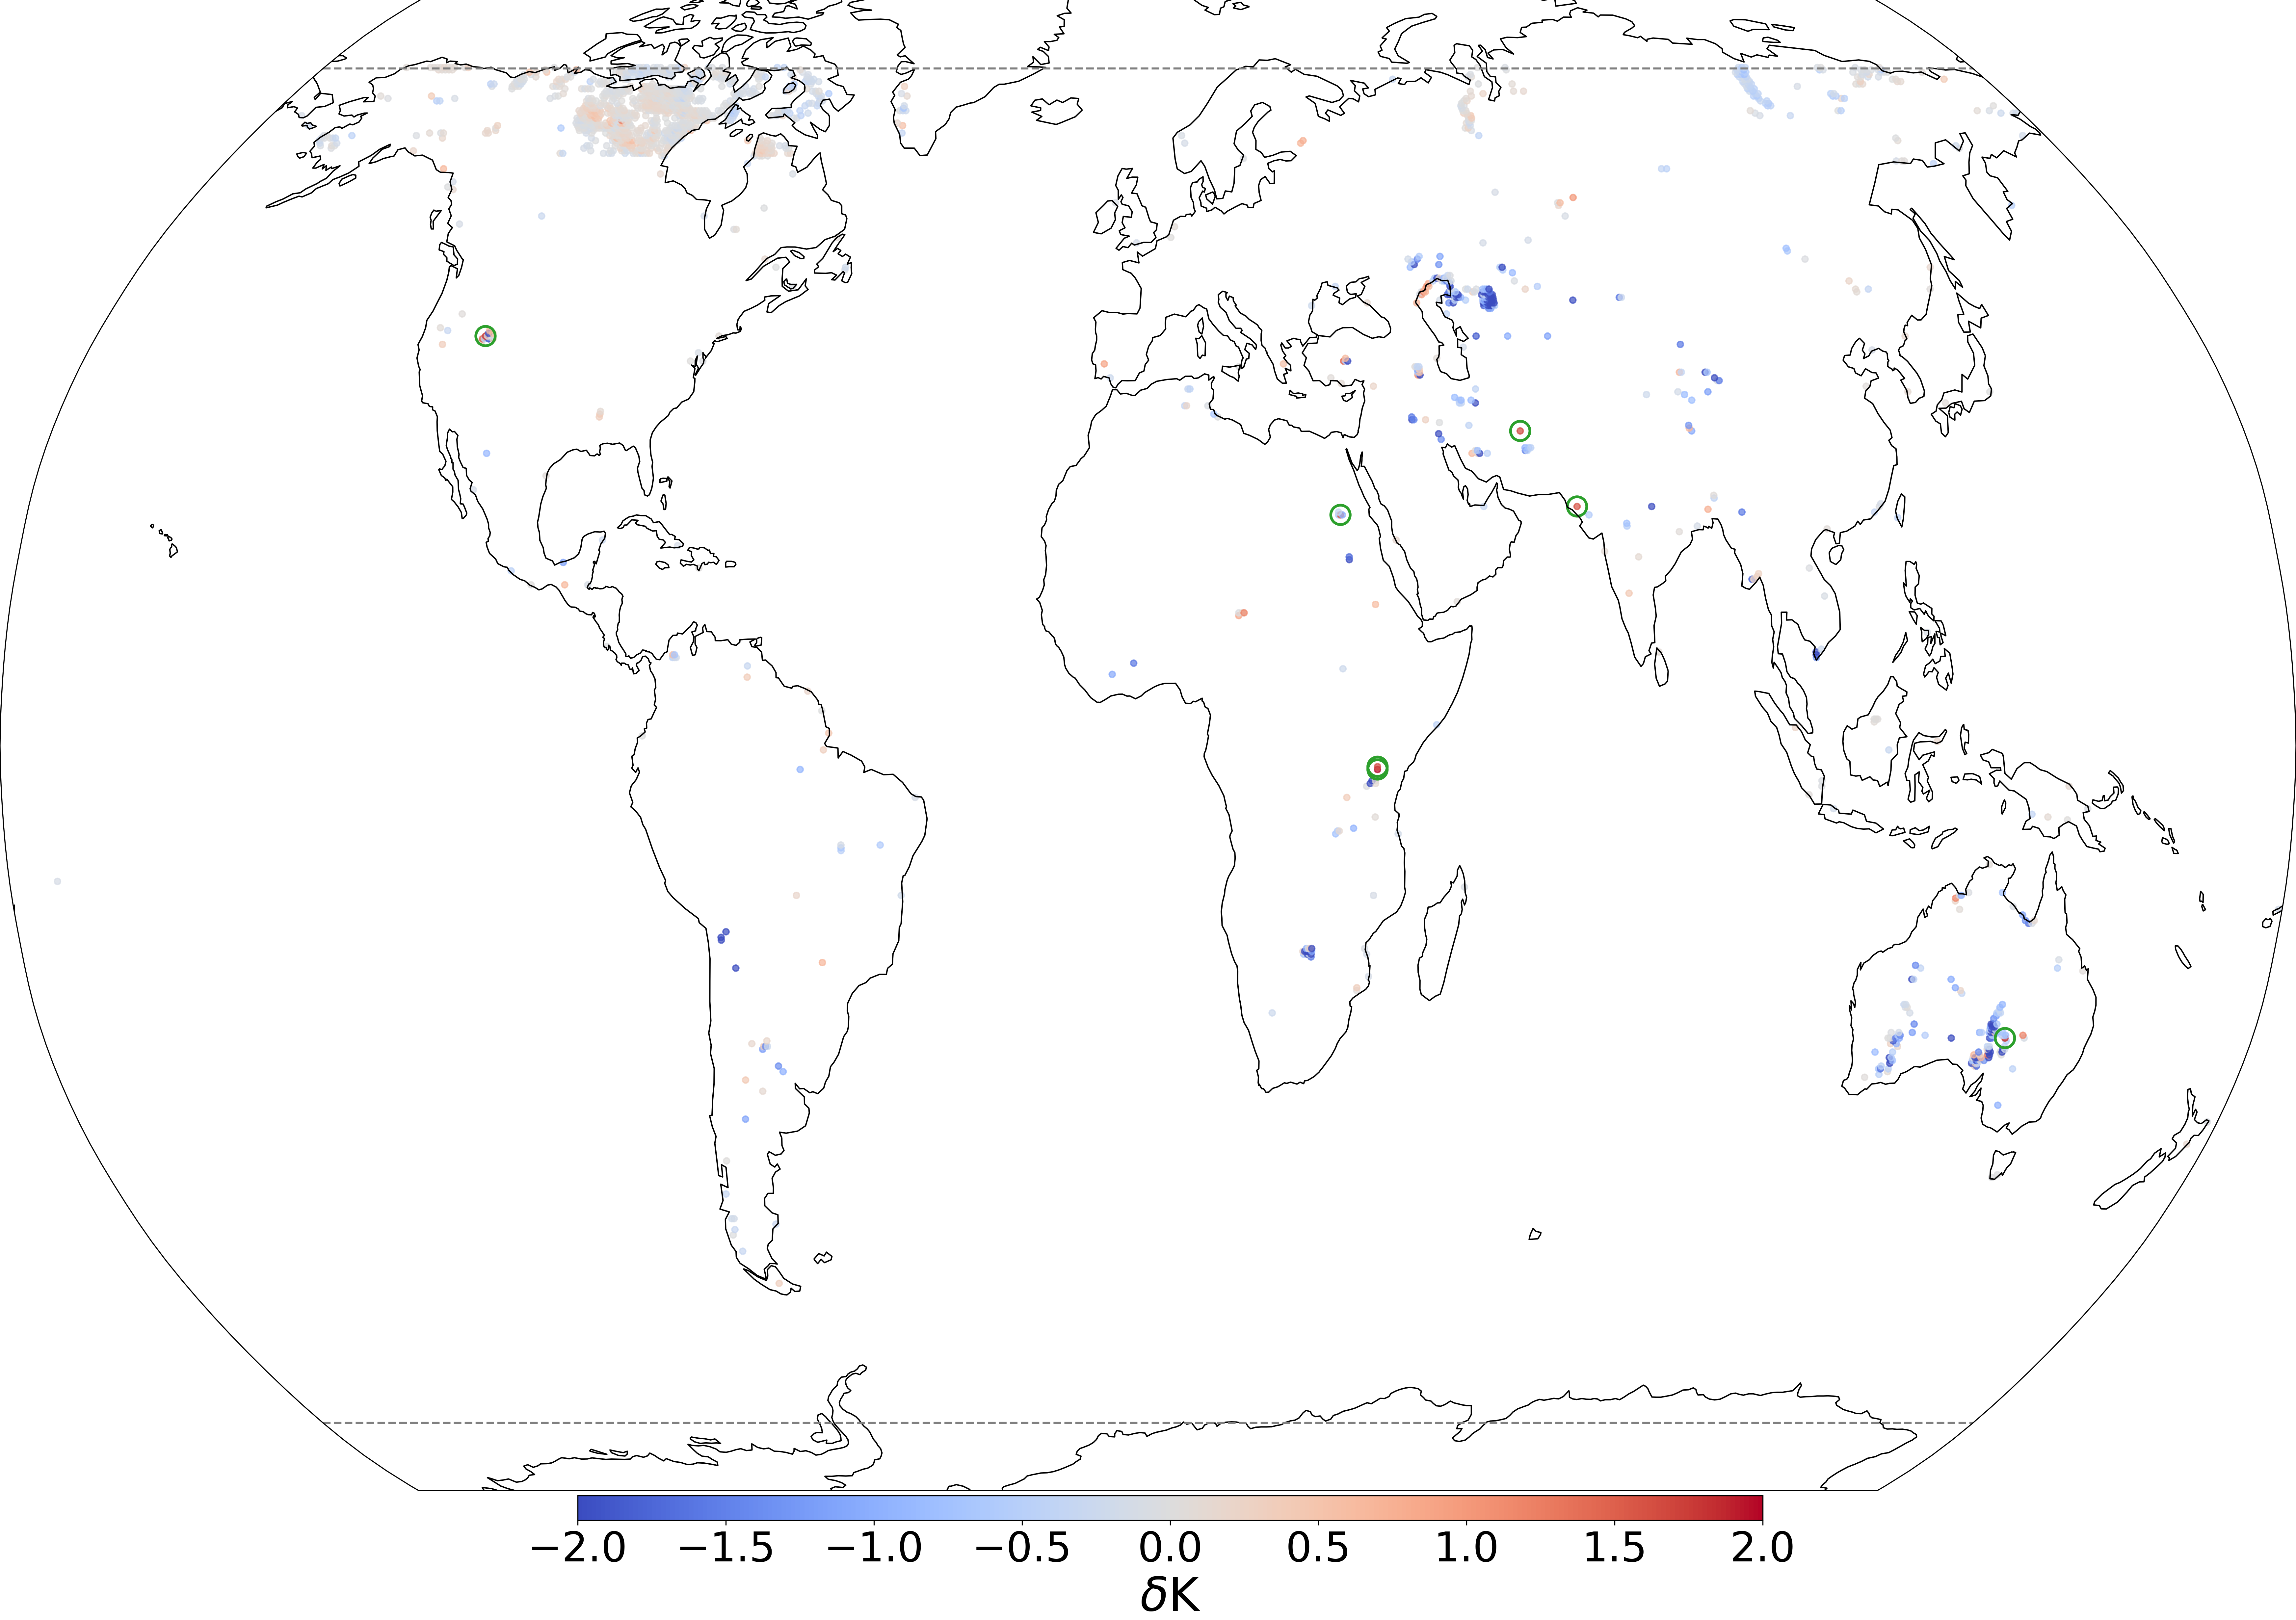
\includegraphics[width=0.98\textwidth]{lake_haver.png}
	\caption{Mean $\delta$ for the V20 model relative to the V15 model across the globe for grid points where all the lake fields have changed significantly (``Lake Update'' category). Generally the updated V20 fields enable the model to make more accurate predictions, for example in the Aral sea and Australia, indicating that these updated fields are informative and accurate. In contrast, there are some regions where the predictions get worse,  for example at higher latitudes which is likely due to these being regions where lakes have more complex, time variable behaviour (e.g. freezing/thawing) and MODIS satellite data is sparse e.g. due to clouds. 7 points (two are overlaid in sub-Saharan Africa) where the V20 prediction gets notably worse than V15 are highlighted with green circles and discussed in the text.}
	\label{fig:bitstring_100110}
\end{figure*}
\noindent The first category where we see significant improvements is for the Lake Updates category. These points are presented in Figure \ref{fig:bitstring_100110}.  We can see that there have been significant improvements globally (the mean improvement in the prediction accuracy when using the V20 fields was 0.45 K, over 1631 grid points), most notably in Australia and the Aral sea. These were two of the major regions that we discussed earlier where in V20 we have removed the ephemeral water (e.g. for Australia) and corrected lake sizes (e.g. for the Aral sea). By providing this updated information to the model that there is less water than initially thought in these regions, the model can then make more accurate predictions. This is a clear example of a verification of the updated fields - it gives us confidence that these new fields are indeed more accurate and are also informative (i.e. predictive) with respect to surface temperatures. In addition to the areas where there is a notable improvement in the prediction accuracy, there are also some noteworthy regions where the predictions get worse (red points in Fig. \ref{fig:bitstring_100110}) suggesting inaccuracies or lack of information in the new fields. We can take a few of the most noteworthy points (highlighted by green circles in Fig. \ref{fig:bitstring_100110}) in turn:
\begin{itemize}
	\item \textbf{Tanzania}. There are two grid points here where the V20 predictions are less accurate, both at Lake Natron, in Tanzania, which lies to the south-east of Lake Victoria. One grid point lies on the northern edge of the lake, and the other is more central. For the central point, the lake fraction was increased from 0.04 in V15 to 0.39 in V20. However Lake Natron is a highly saline lake that often dries out, with high temperatures, high levels of evaporation and irregular rainfall. It is a highly complex and variable regime that is not well described by simply increasing the static lake fraction field, and indeed these results suggest that it may in fact be beneficial for the current lake parametrisation scheme to keep the lake fraction low here (see e.g. Fig \ref{fig:lakes1}). Similar arguments apply for the grid point at the northern edge, where the lake fraction has also been increased, along with a small decrease ($\sim 0.1$) in \textit{cvl}. 
	
	\item \textbf{Australia}. This grid cell lies in South Australia and contains Lake Blanche. In going from V15 to V20 all water was removed, with the lake fraction decreasing from 0.44 to 0 and the lake depth reduced from 5.5m to 1m. This water is then replaced with vegetation; the low vegetation fraction \textit{cvl} increasing from 0.53 to 0.97. Whilst the removal of ephemeral water is generally accurate for Australia, for this grid point it causes the V20 predictions to become worse. Lake Blanche is a salt lake that lies within a wetlands system and so will retain some surface water which will influence the temperature response. The lake itself also lies below sea level, but the orography fields in V15 or V20 do not reflect this. Satellite imagery (e.g. Fig \ref{fig:lakes2}) suggests that the area surrounding Lake Blanche is also fairly devoid of any obvious vegetation. The V20 description of a completely dry region covered short grass (low vegetation) is then insufficiently accurate, and results in worse predictions. 
	
	\item \textbf{Salt Lake City, North America}. This grid point lies just to the west of the Great Salt Lake, Utah, within the Great Salt Lake Desert. All water was completely removed when going from V15 to V20 (\textit{cl} from $\gtrsim$ 0.5 to 0). The V20 model then treats this region simply as bare ground. Whilst this area primarily is bare ground, satellite imagery also suggests the presence of a presumably highly saline lake (Fig \ref{fig:lakes3}).This region also has a large degree of orography and high elevation ($\sim 1300$ m) which will also further complicate the surface temperature response. Again, a more accurate description that accounts for the seasonality of the surface water and the salinity is necessary here.
	
	\item \textbf{Afghanistan}. This grid point lies in the south west of Afghanistan, close to the border with Iran. The only notable change when updating from V15 to V20 was the removal of the water, with the lake fraction decreasing from 0.11 to zero. However, this area in fact has an extensive network of mountain tributaries which feed an ephemeral lake (e.g. Fig. \ref{fig:lakes4}). There is therefore likely some surface water for parts of the year, especially during the rainy season, and completely removing all water for this grid point  is an overcorrection.
	
	\item \textbf{Northern India}. This grid point lies in the state of Gujarat, close to the border with Pakistan. The lake fraction \textit{cl} was increased from 0.59 to 0.71 and the lake depth \textit{dl} increased from 2.58m to 3.76m. That is, the V20 corrections suggest that there should be a larger degree of lake cover in this grid box. However, this point appears to lie on a river delta within the Great Raan of Kutch, a large area of salt marshes (Fig \ref{fig:lakes5}). This area is known to have highly seasonal rainfall, with frequent flooding during the monsoon season and a long dry season. The surface itself also undulates with areas of higher sandy ground known as \textit{medaks}, with greater levels of vegetation. It is evidently a complex and highly time variable area and the additional static information provided via the V20 fields is either not accurate or not predictive/informative enough in such a variable regime.
	
	\item \textbf{Egypt} This grid point lies in the south of Egypt, to the west of the River Nile. Again, all water has been removed from this region, with the lake fraction reducing from 0.36 in V15 to zero in V20. The lake depth has been similarly decreased from 25m to 6m. However, whilst this is a very dry region, this grid cell also contains a section of the Toshka Lakes (Fig \ref{fig:lakes6}), a collection of endoheic lakes, newly formed (and growing) due to overflow from Lake Nasser. These lakes are known to be highly time variable, with a periodic seasonality on top of the general increasing lake sizes, and the formation of surrounding wetlands. These lakes rapidly fill and dry out; during the training and validation years -  along with the decade before - the lakes were mostly dry\cite{ToshkaURL}, whereas during the testing year they were filled.
\end{itemize}
\noindent Whilst these are the major regions where the V20 prediction is significantly worse than the V15 prediction, there are other regions of note where the underperformance is less severe. For example in parts of northern Canada there is a notable population of red points, where for the Northwest Territories the mean $\delta_{\rm V20}$  is +0.02K. This difference is slight and it is hard to draw any definitive conclusions - whilst some grid points get better, some get worse. For these high latitude regions there is a large variability over the course of the year as the water freezes in the cold season and then melts during the summer. Such a time variability is not ideally captured by lake parametrisation which is likely the cause of the issues here, along with the greater uncertainty and error in the observations in these regions with increased cloud cover. Another interesting location is the north eastern edge of the Caspian Sea, where there are 4 grid points with a mean $\delta_{\rm V20}=+0.65$K. This is the Astrakhan Nature Reserve, an extensive wetlands region. In going from V15 to V20, the lake fractions have generally been decreased and the vegetation fractions increased correspondingly. However, since these are wetlands there is likely a large degree of water present and the updated V20 lake fields may be insufficiency informative and an extra map of wetlands may be necessary. \newline 


\noindent We can also inspect the subclass of the Lake Updates category, Lake-Ground Updates, and restrict our analysis to only points where there was no significant change in the vegetation. This then allows us to more clearly see the effect of adding/removing water without the additional influence due to the change in vegetation. In this case the mean improvement in the prediction accuracy when using the V20 fields is stronger than the Lake category, with $\delta_{\rm V20} = -1.12$ K. This indicates that whilst the updated lake fields are globally accurate and informative, providing on average over the globe, over a year, more than an extra Kelvin of predictive performance, the updates to the vegetation fields tamper this performance gain. This suggests at a potential problem with the vegetation fields, which we will now explore further.

\begin{figure*}
	\centering
	\subfloat[Lake Natron, Tanzania \label{fig:lakes1}]{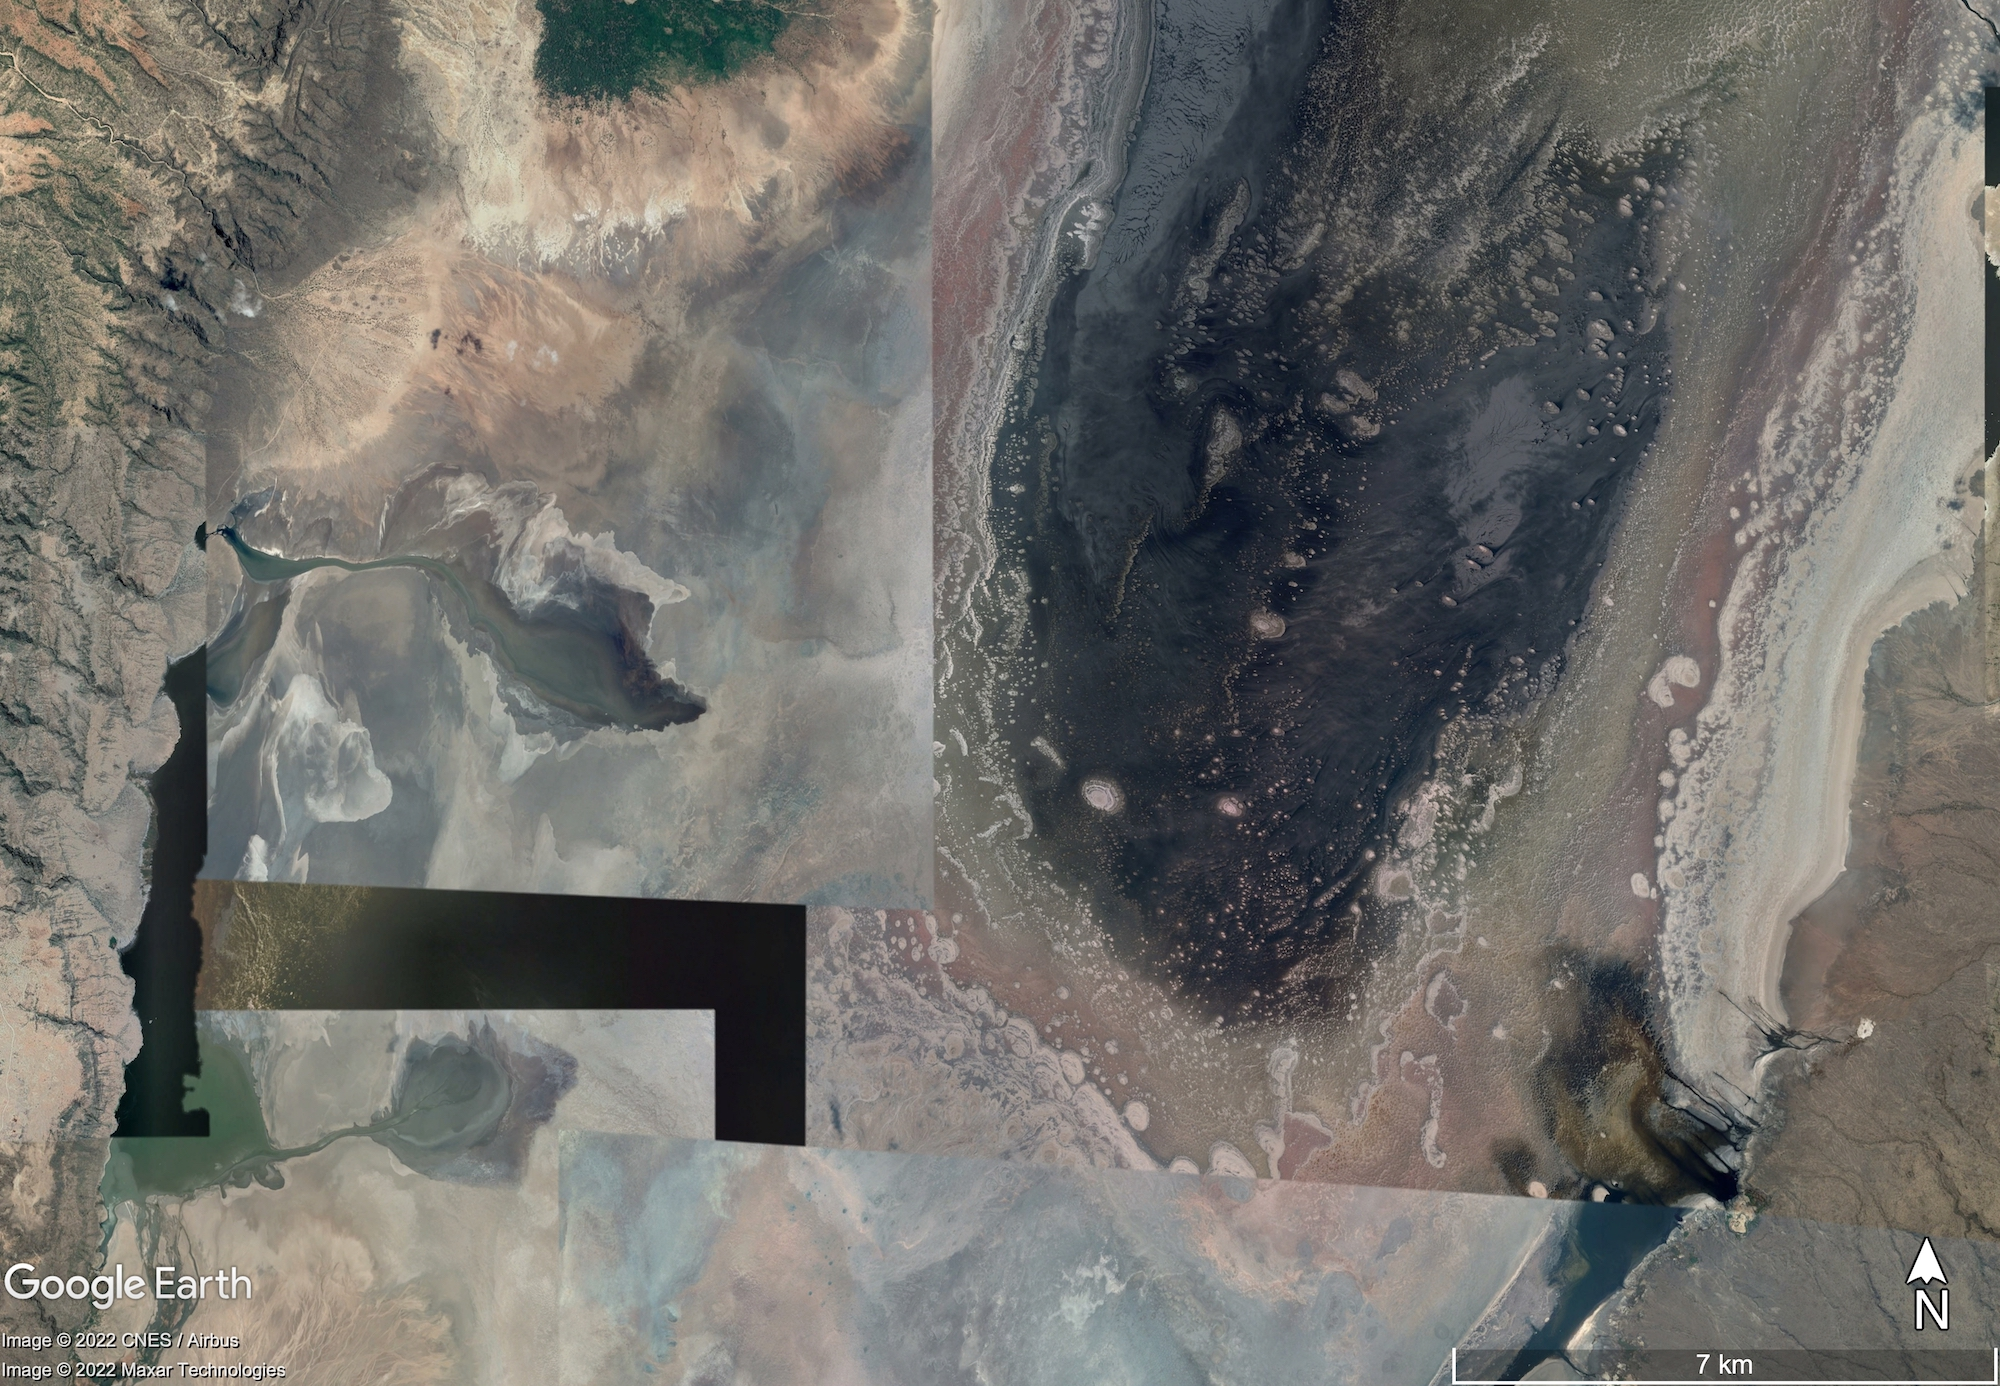
\includegraphics[width=0.45\textwidth]{LakeNatronCentre4.jpg}} \hspace{1mm}
	\subfloat[Lake Blanche, Australia \label{fig:lakes2}]{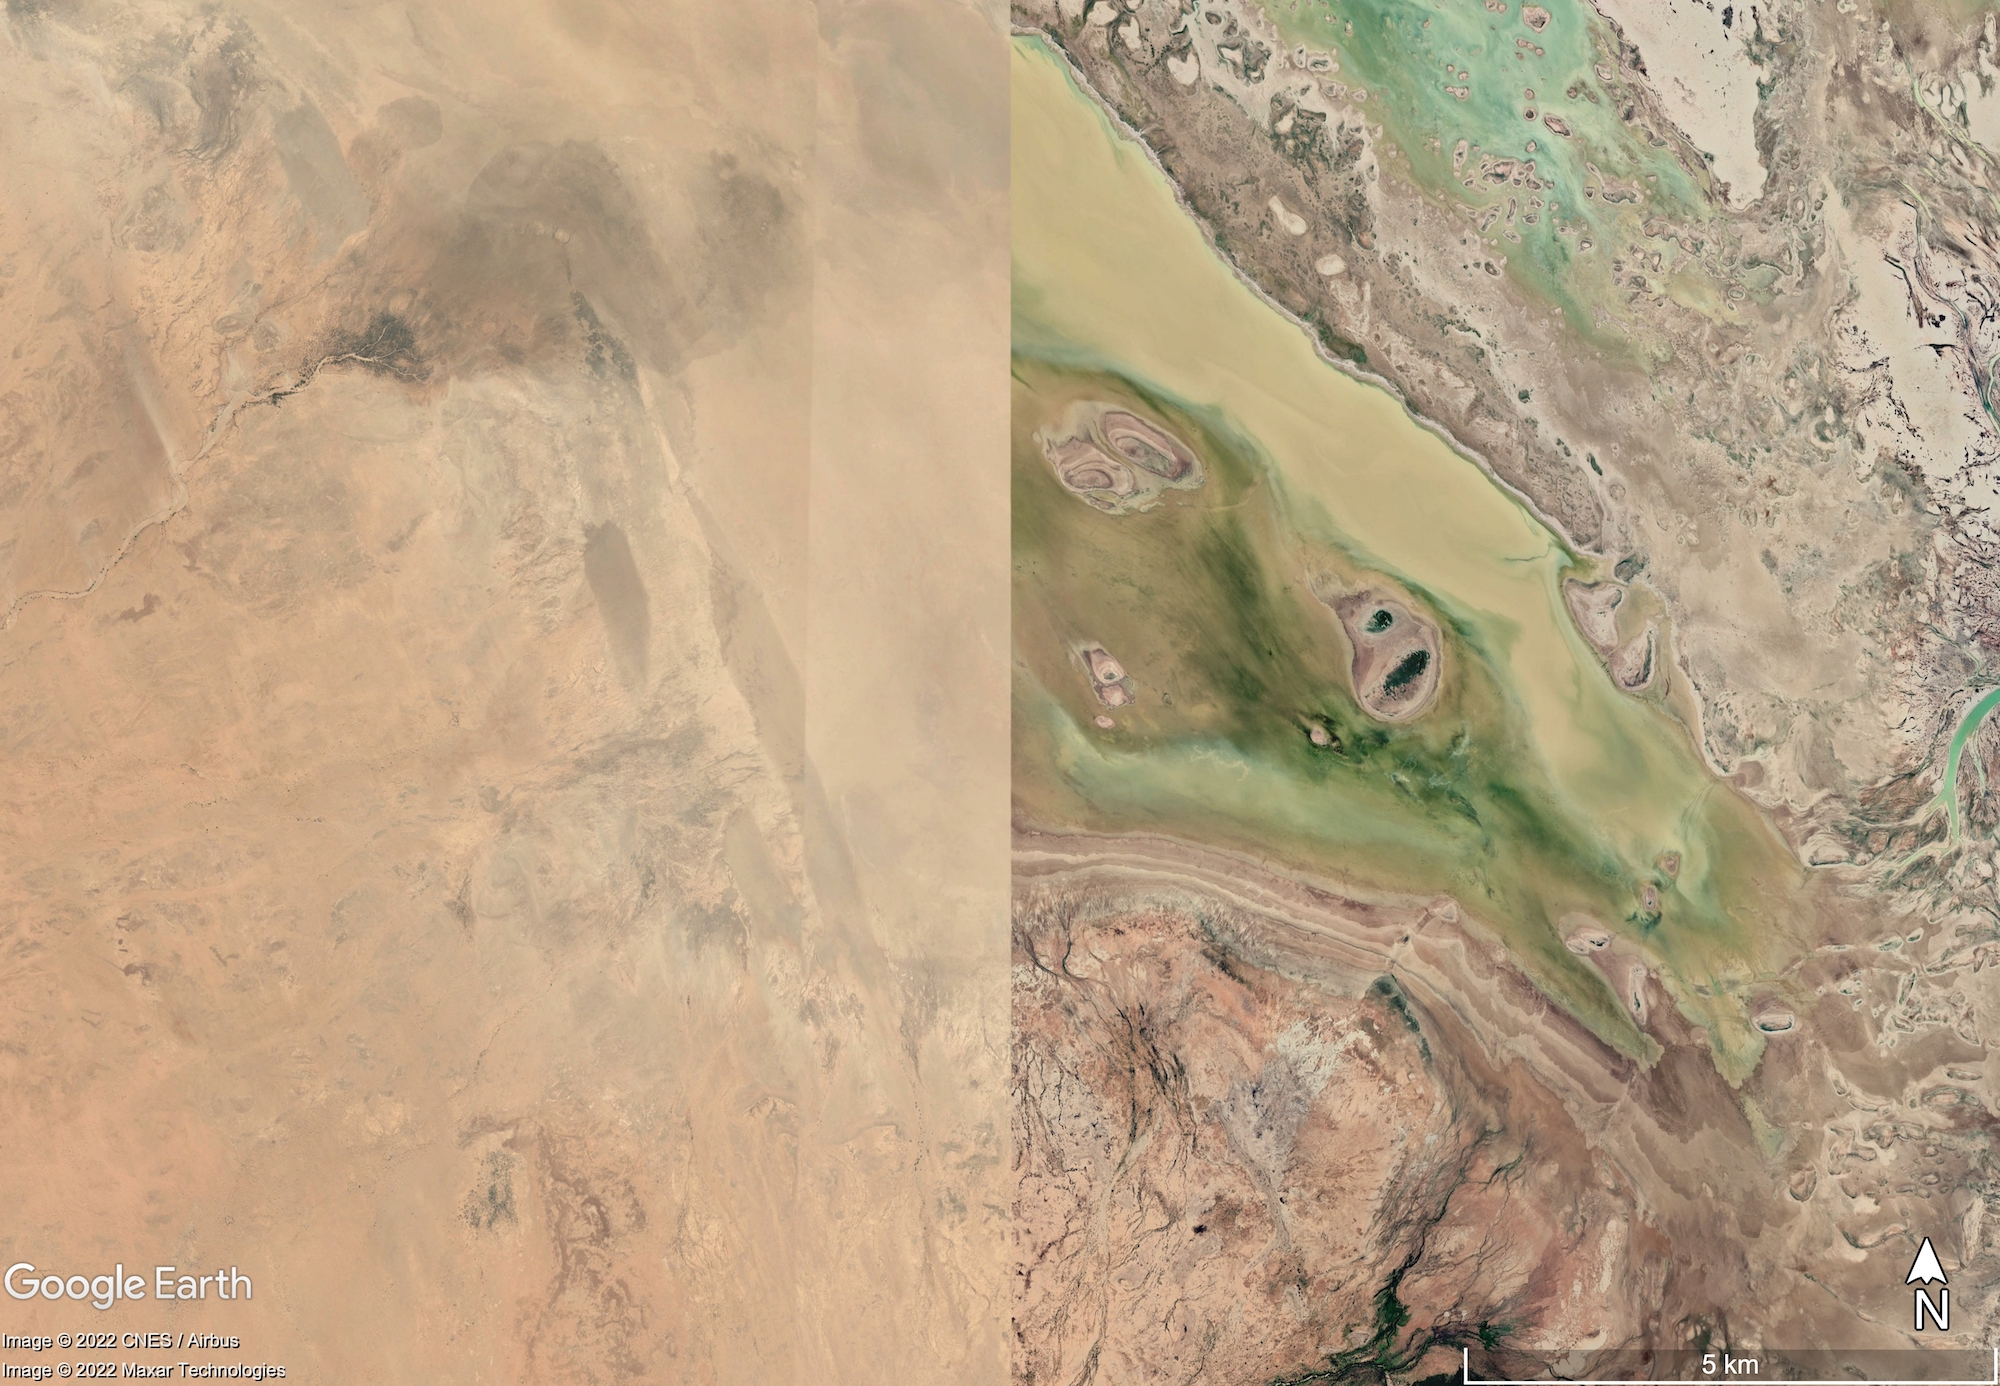
\includegraphics[width=0.45\textwidth]{Australia1}} \\
	\subfloat[Great Salt Lake Desert, Utah\label{fig:lakes3}]{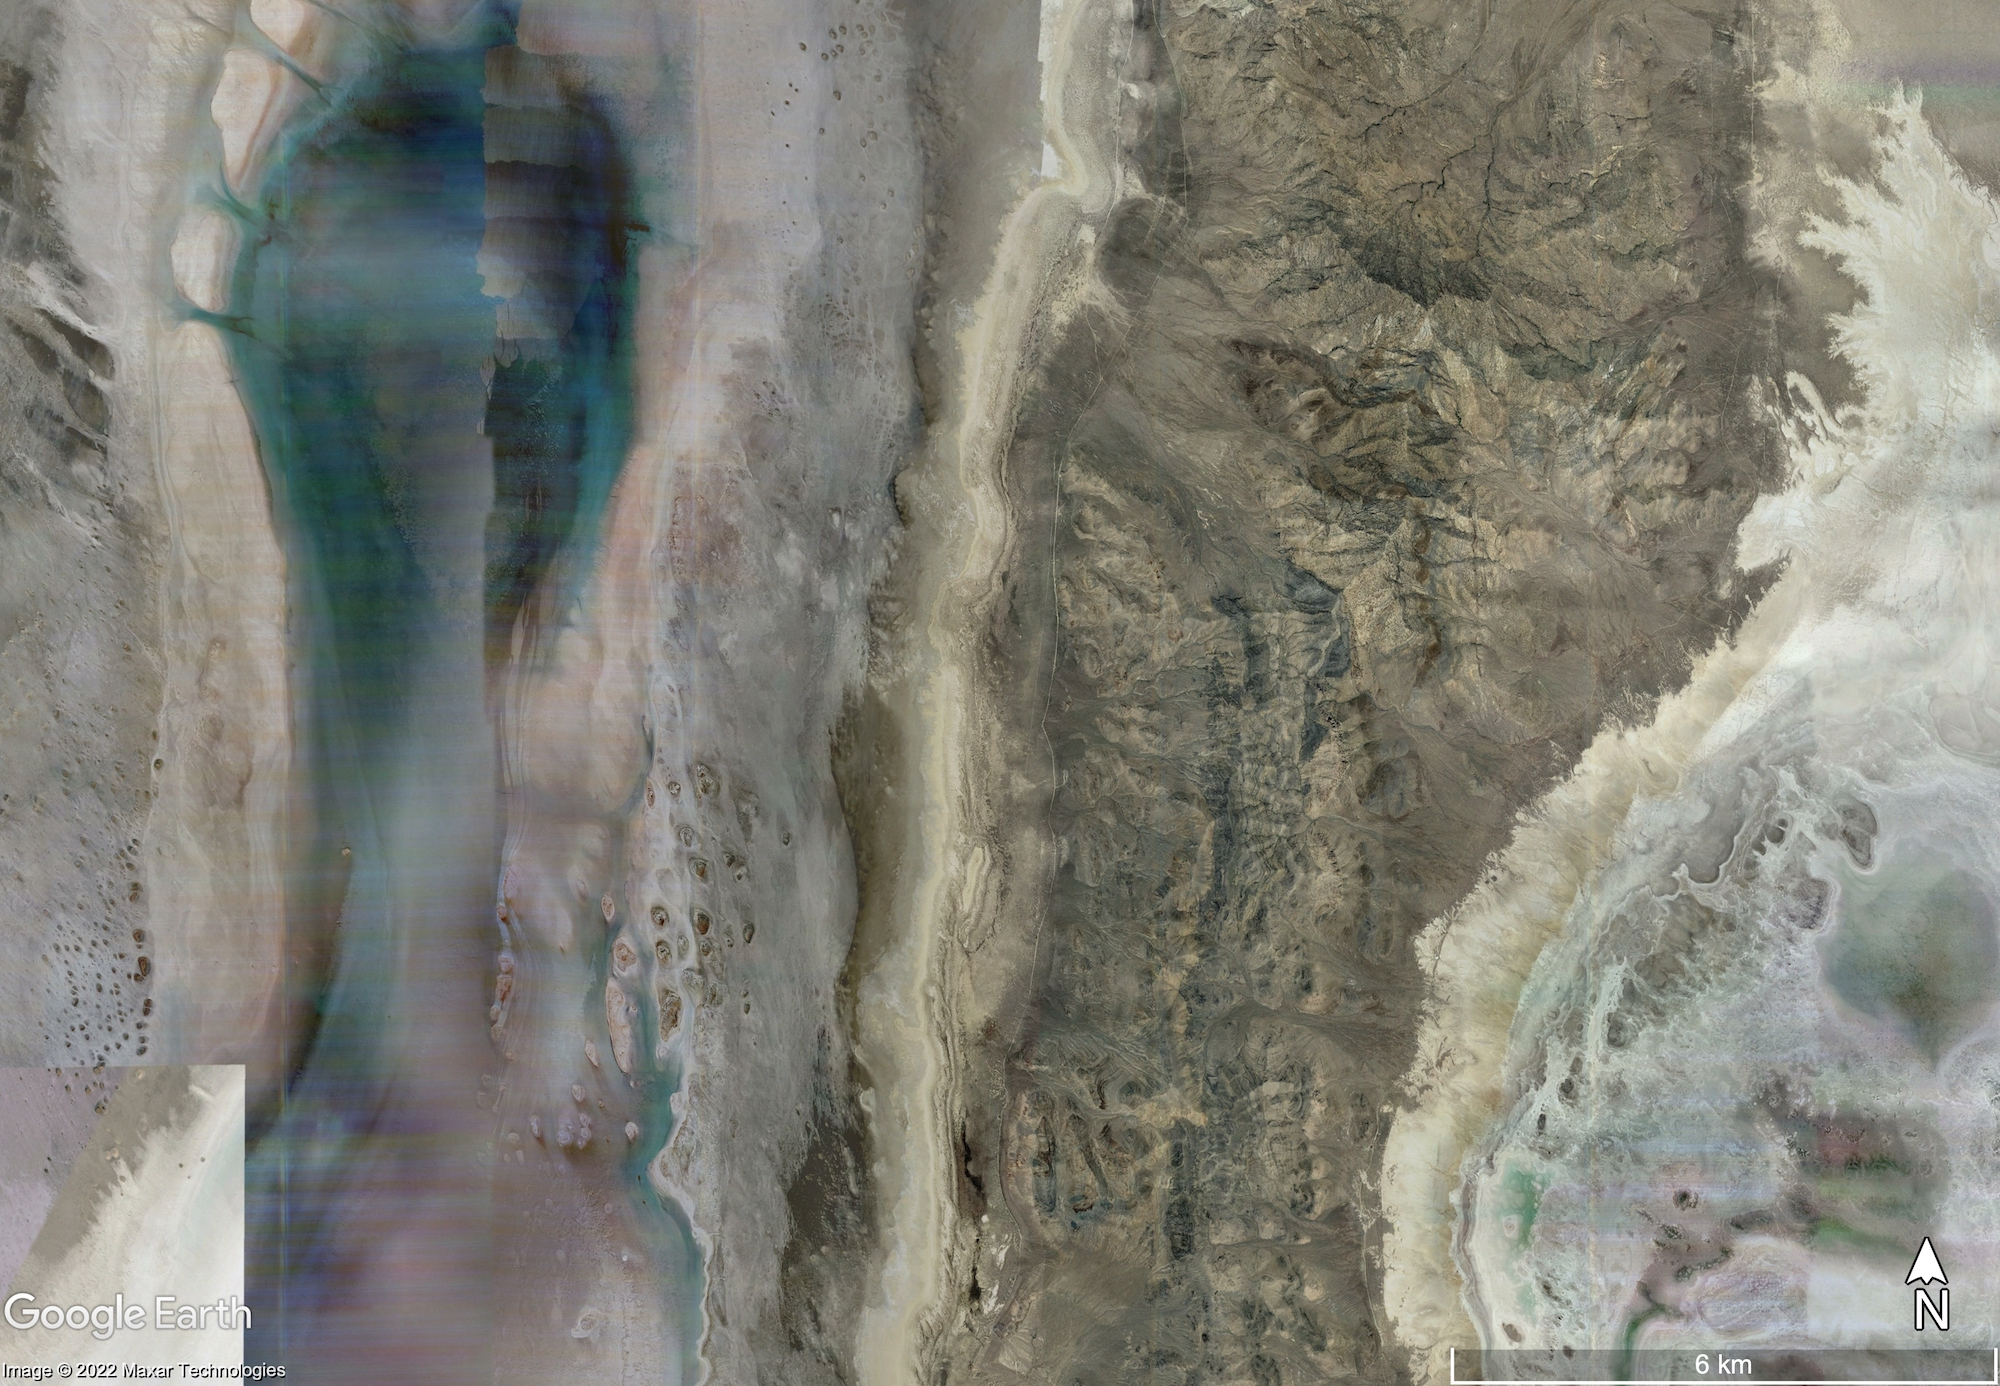
\includegraphics[width=0.45\textwidth]{SLC1.jpg}} \hspace{1mm}
	\subfloat[Farah Province, Afghanistan\label{fig:lakes4}]{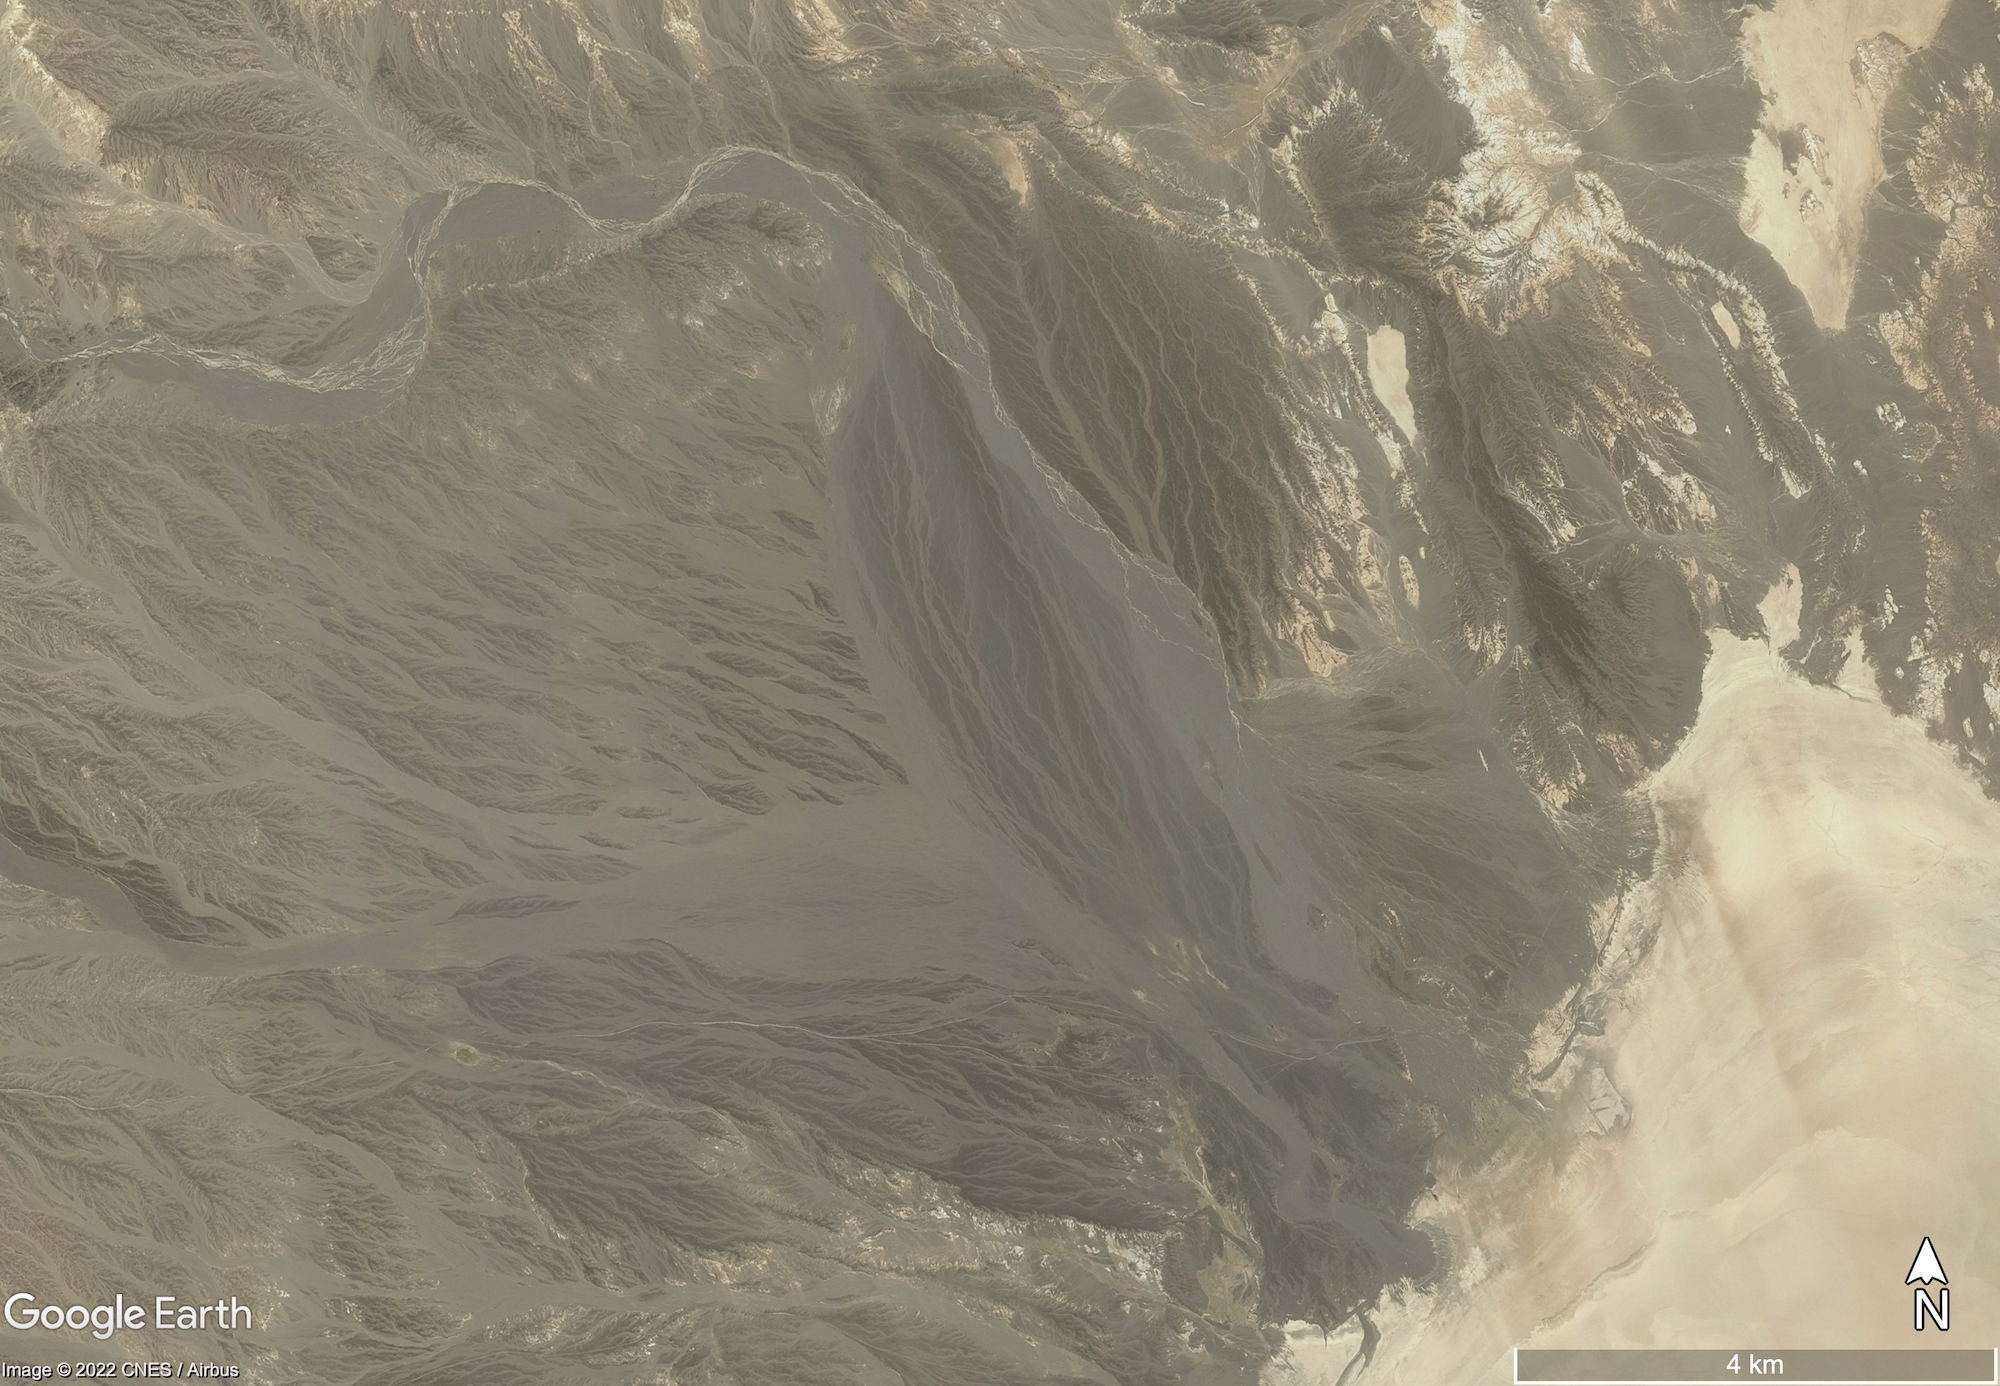
\includegraphics[width=0.45\textwidth]{Afghan1}} \\
	\subfloat[Gujarat Province, India\label{fig:lakes5}]{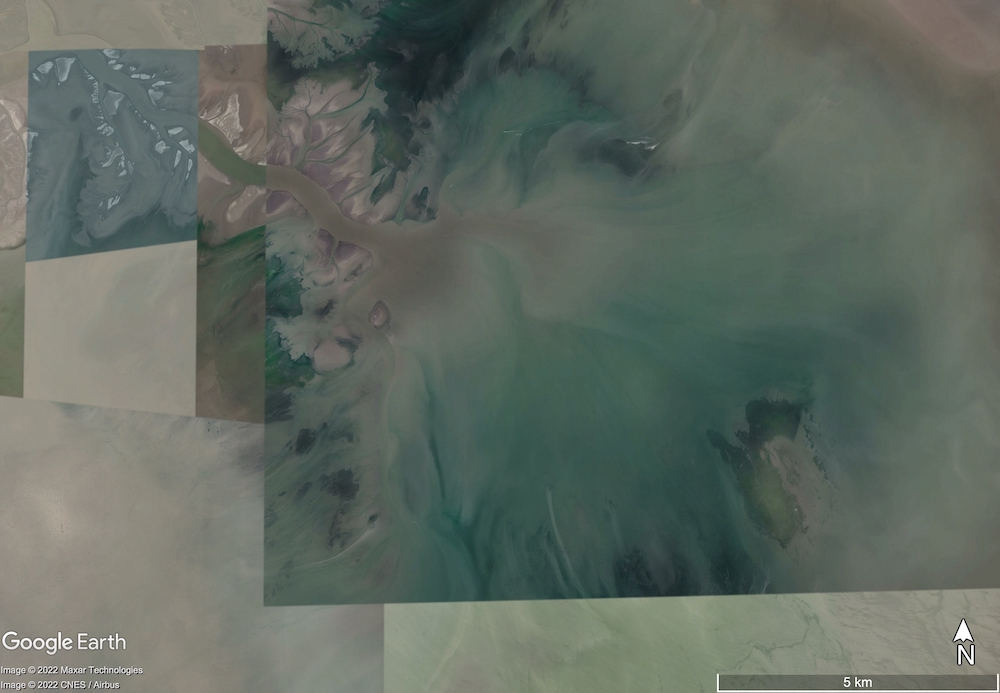
\includegraphics[width=0.45\textwidth]{India1.jpg}} \hspace{1mm}
	\subfloat[Toshka Lakes, Egypt\label{fig:lakes6}]{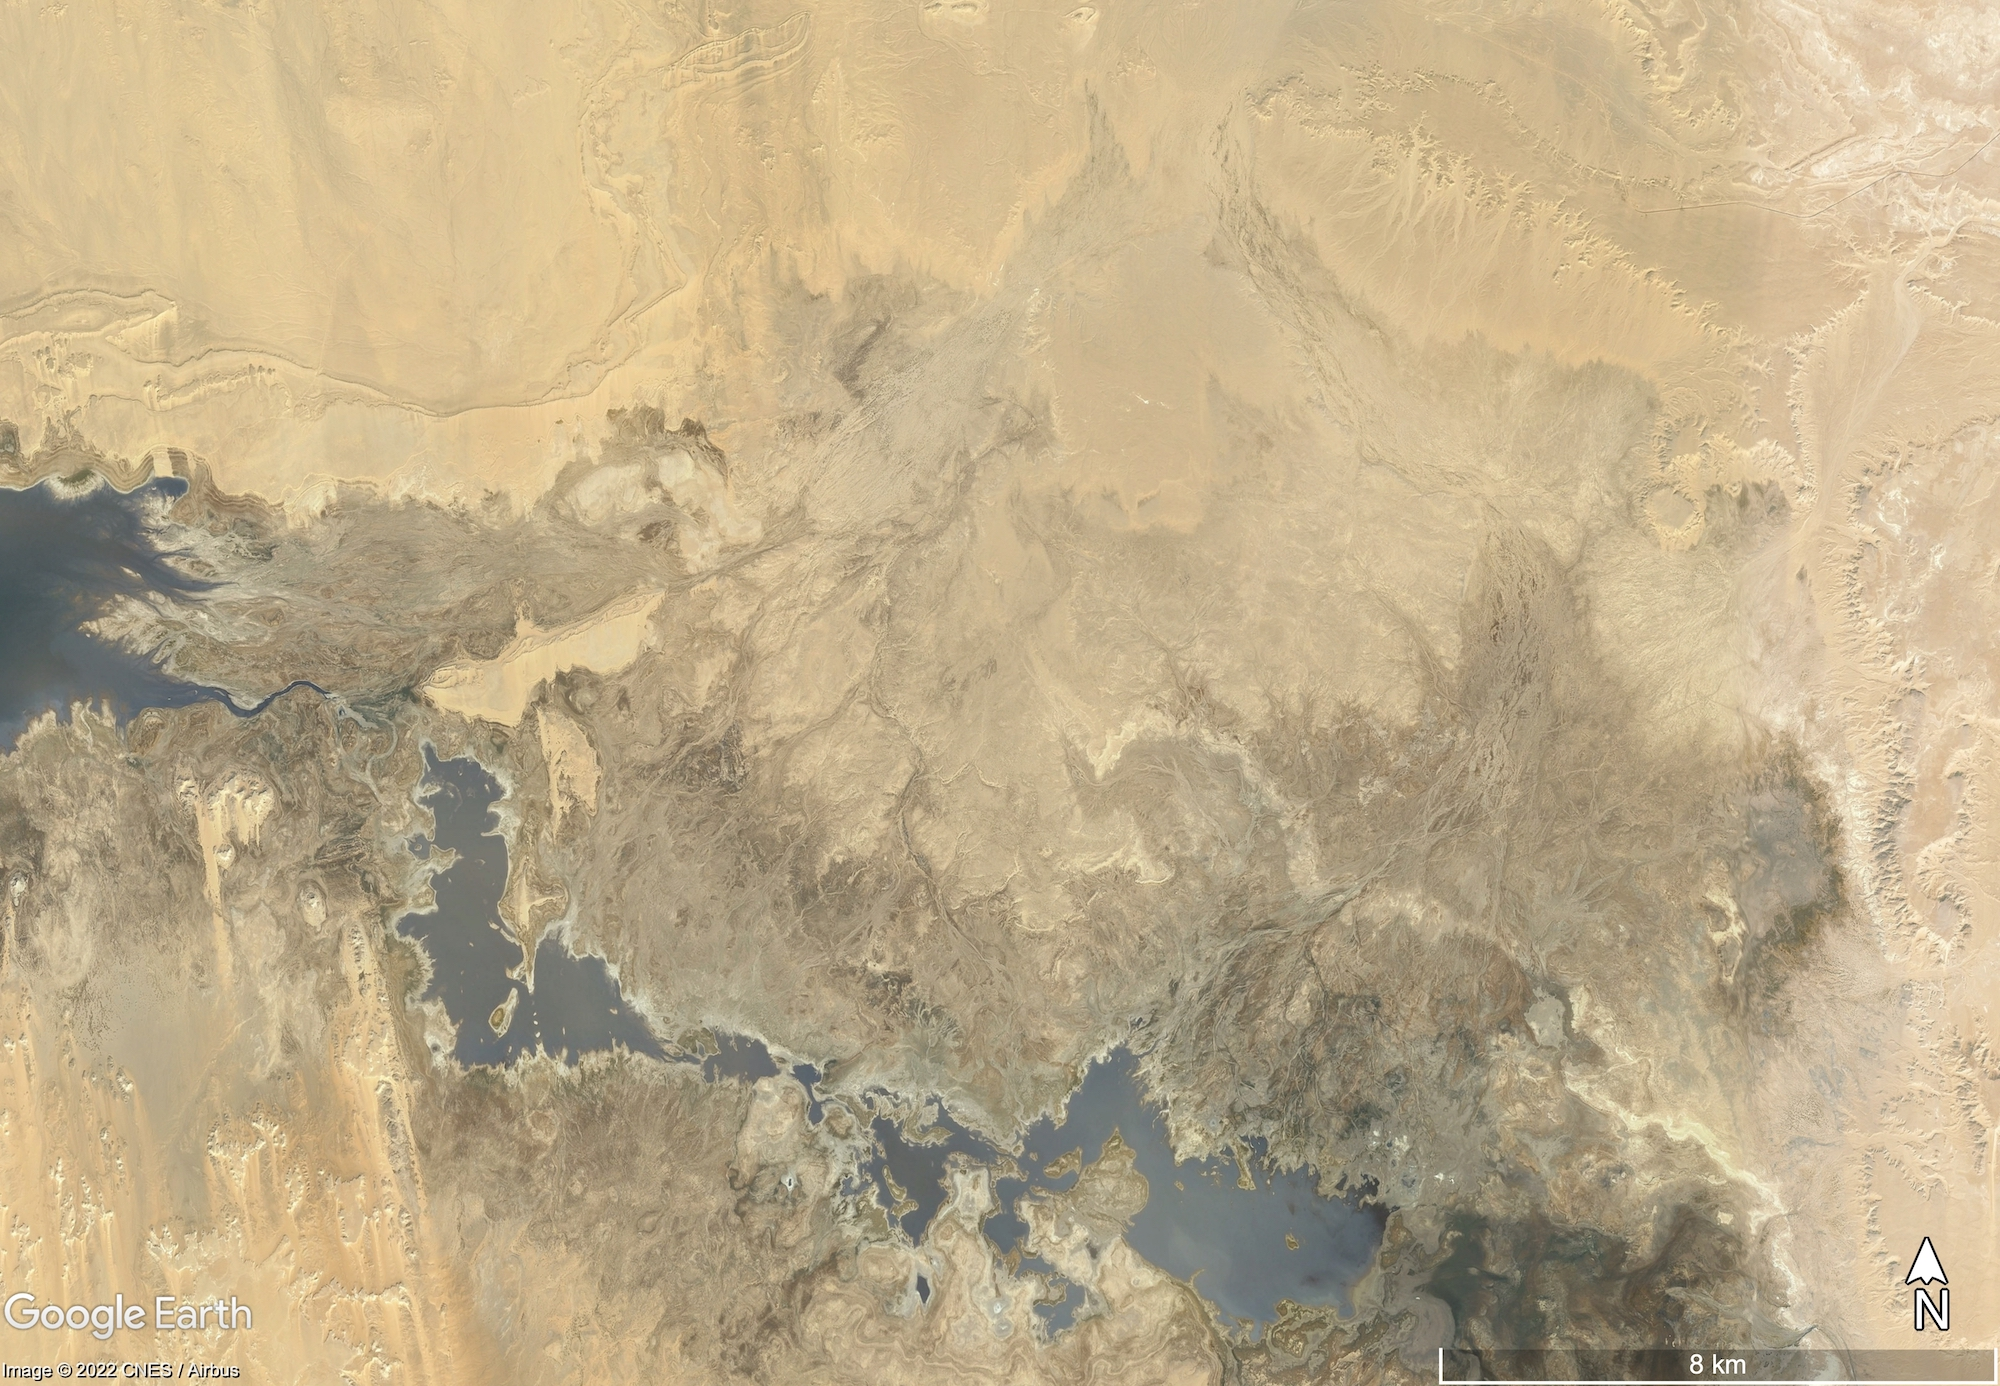
\includegraphics[width=0.45\textwidth]{Egypt1}}
	\caption{Satellite imagery of the problematic Lake Updates points highlighted in Fig. \ref{fig:bitstring_100110} where the V20 predictions are worse than the V15 predictions. Generally the updated V20 fields remove water, only considering permanent water. However these regions have highly time variable waters, which are better captured on average by the V15 fields. The images are centred on the grid box coordinates. Note that the lengthscales are different for some images.} 
	\label{fig:example_test}
\end{figure*}


	
	
	\subsubsection{Category: Vegetation Updates}\label{V20Vegetation}
	Whilst the edits to the V15 lake fields generally act to increase the prediction accuracy, indicating that these fields are accurate and informative, changes to the vegetation generally give worse predictions. We can see from from Table \ref{tab:V1520_results} that the mean prediction accuracy when using the updated fields decreases by 0.49K over 58 points. For all points apart from one, the \textit{cvh} fraction was decreased, often quite drastically to zero, i.e. specifying that there should just be bare ground in these grid boxes. Whilst this may be accurate for some points, by inspecting these areas with satellite imagery it is clear that there are regions which are in fact areas of high vegetation (e.g. Fig \ref{fig:cvh}) and that it is inaccurate to simply remove all vegetation from these grid boxes. It is also notable that the  grid points which have the largest drop in predictive performance when going from V15 to V20 are all grid points where the vegetation fraction is severely reduced to zero. This suggests that such extreme changes may be strong over-corrections, and more modest updates to the vegetation fields may be more accurate. These erroneous V20 vegetation fields are likely inherited from  initial datasets used to update vegetation or during the interpolation. The errors in these regions will in turn corrupt the LST predictions and mitigate the gain from a more accurate representation of the lake water.
	\begin{figure}[h!]
		\subfloat[\label{fig:cvh1}]{\includegraphics[width=0.48\textwidth]{siberut_hr.jpg}} \\
		\subfloat[\label{fig:cvh2}]{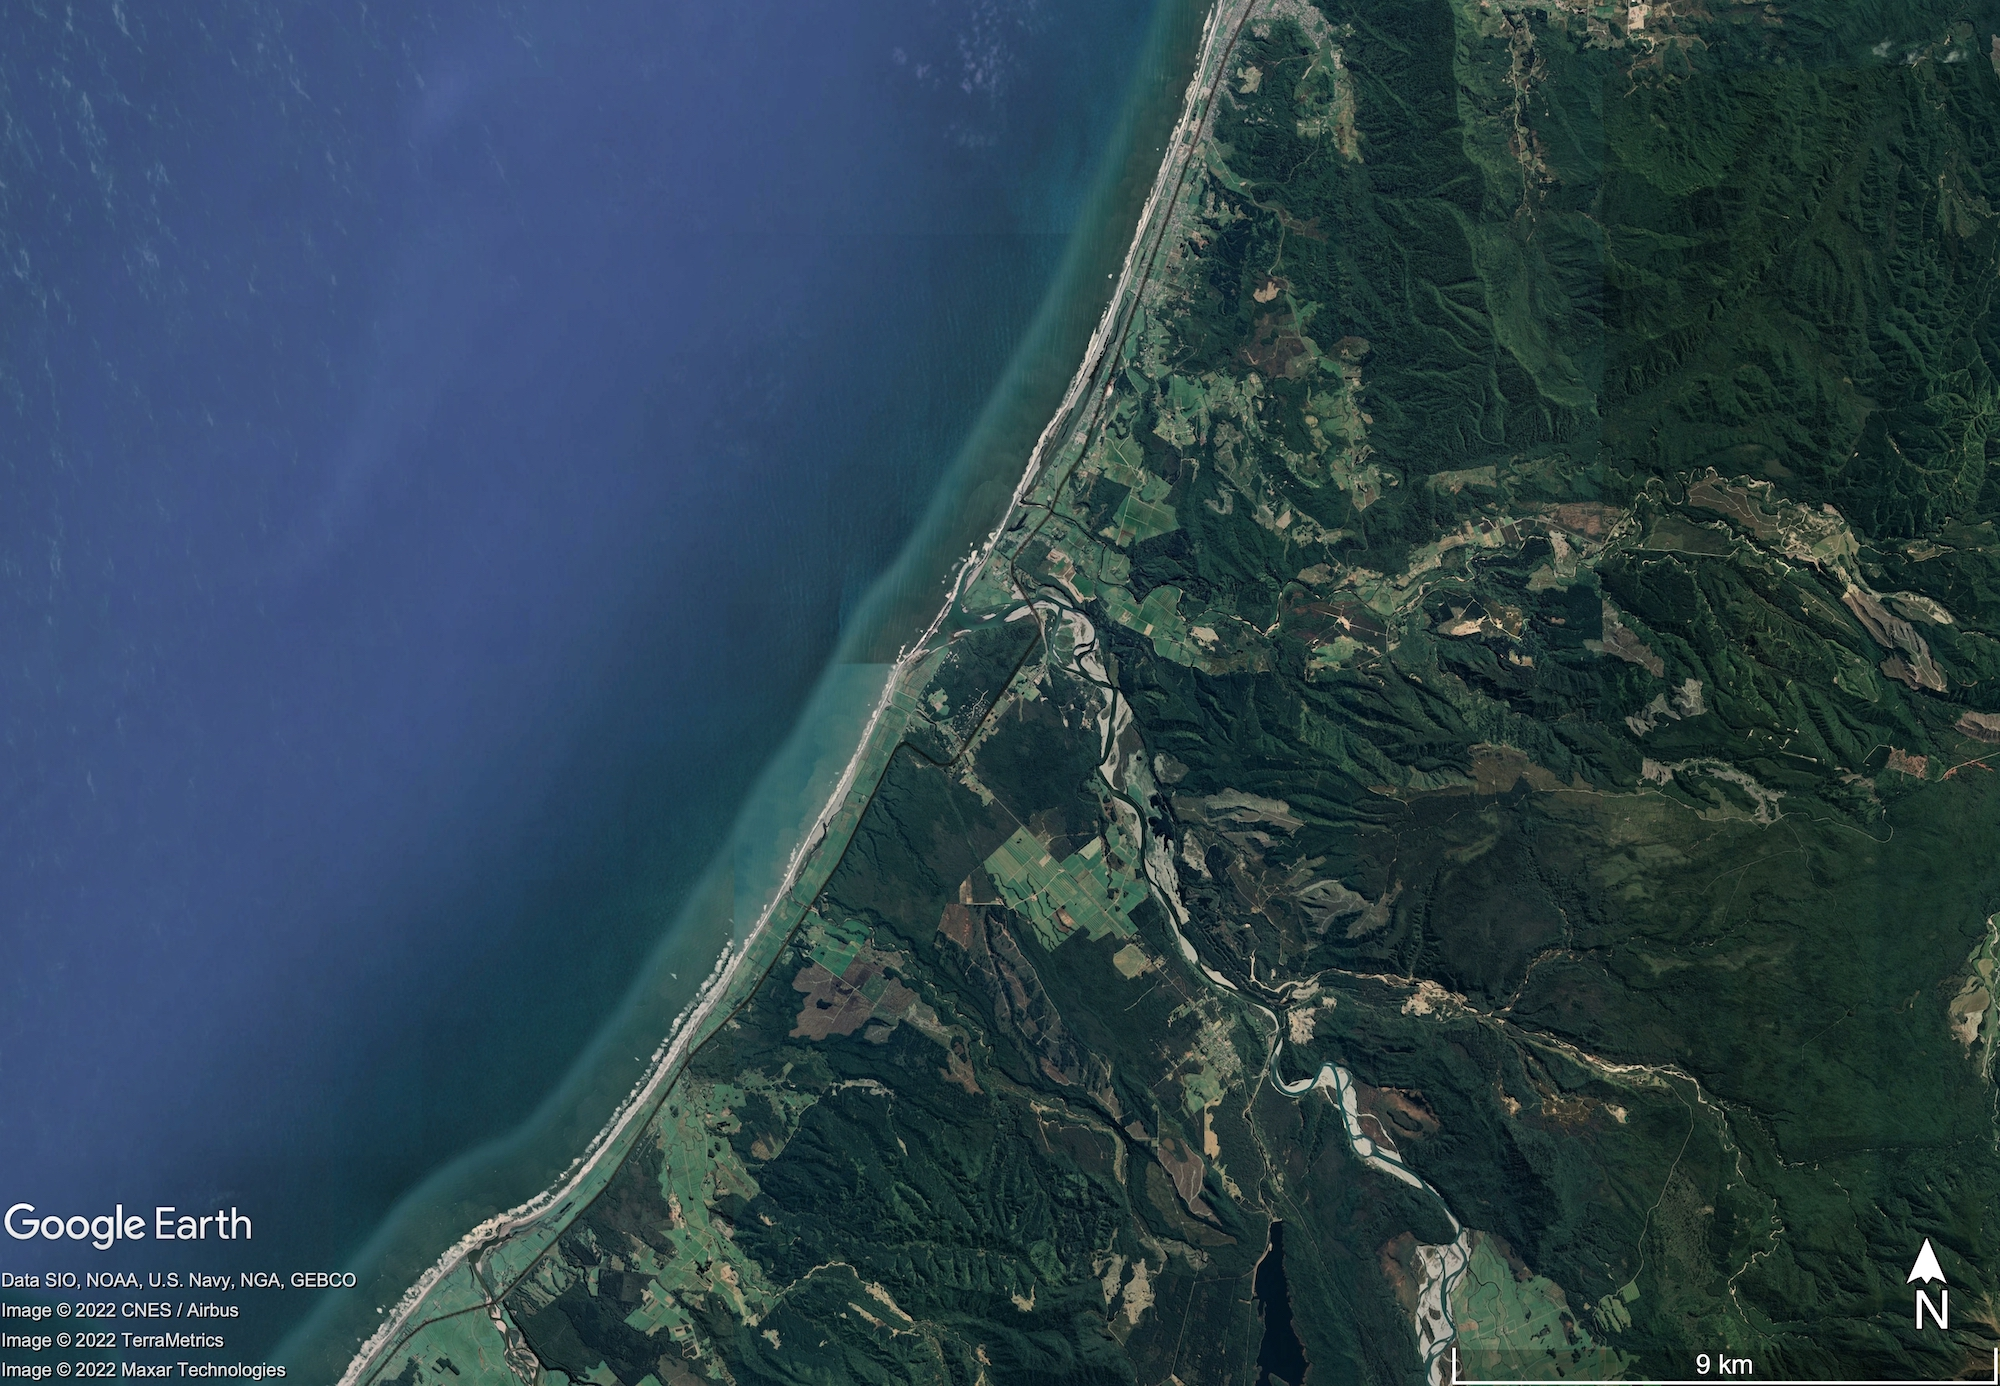
\includegraphics[width=0.48\textwidth]{NewZealandVeg.jpg}} 
		\caption{Satellite imagery of grid boxes in \textit{(a)} Siberut Island, Indonesia  and \textit{(b)} South Island, New Zealand. For both points it is expected according to the updated V20 fields that there is no vegetation, just bare ground. VESPER can identify these erroneous updated fields.} 
		\label{fig:cvh}
	\end{figure}
	
	
	\subsubsection{Category: Glacier Updates}\label{V20Glacier}
	The V20 updates to the glacier fraction also generally improve the predictions, with a mean $\delta_{\rm V20} = -0.14$ K over 1057 grid points. These improvements are concentrated around the Himalayas, the land either side of the Davis strait, as well as British Columbia and the Alaskan Gulf. Analogous to the Lakes Updates category whilst the introduction of the V20 fields generally improves the model, there are some selected regions where the  prediction gets worse. These are heavily concentrated in the southern hemisphere, in particular on the south western edge of South America and the South Shetland Islands - which lie closer to Antarctica - as well as some parts of the Himalayas. This deficit in performance in these areas is not due to erroneous updated V20 fields, but instead is a data quality issue whereby we do not have a lot of MODIS observations in these areas which have a large degree or orography and cloud cover. This can be seen in Fig \ref{fig:MODIS_obs} for the above mentioned regions. Consequently the neural net model finds it difficult to make accurate predictions in this region, and this iteration of the model has settled into a local minimum for V20 which is worse than V15 in these areas. If we isolate just grid points where we have a large number of observations (we take mean number of MODIS  observations per ERA data point $> 50$) then the worst performing grid points are excluded. In this case there do remain a few areas where the V20 model underperforms with respect to V15. For example there is a grid point in the Alaskan gulf on the Bering Glacier with $\delta_{\rm V20} = +2.16$ K. This point has been updated in V20 to have a higher glacier proportion (0.68 to 0.92), such that the grid box should be almost completely dominated by ice. Nearly all low vegetation was also completely removed (\textit{cvl} from 0.10 to 0.007) and the lake depth increased from $\sim 2$m to $\sim$27, in conjunction with a modest decrease in the lake fraction, from 0.07 to 0.01. Satellite imagery of the region (Fig. \ref{fig:glacier}) shows an area that does have a significant ice fraction, but perhaps not as great as $\gtrsim 90 \%$, suggesting that the V20 updates may have been an over correction. The Bering glacier is also known to be a time variable region which varies in size over the course of the season, whilst on longer timescales exhibits a general retreat of the terminus over time, coupled with periodic surges in the glacier flow around every 20 years \cite{Bering2010}. It is therefore a complex region not necessarily well represented by a static fractional field. There also appears to be some low level vegetation present, and again removing all vegetation for this region may have been an overcorrection. Another notable grid point is in the Chilean Andes, by the Juncal Glacier. Here the ice fraction was increased in V20 to 0.25 from zero in V15, an attempt to better represent the glacial ice. However, $\delta_{\rm V20} = +2.67$K. In fact, the glacier itself only occupies a small fraction of the overall grid box, and the updated field may have been an over correction. Moreover, this is an area with lots of orography, with snowy mountains at high altitude and deep valleys. Therefore the temperature response due to the glacier feature could be atypical compared to e.g. the Alaskan Gulf or the Davis straight. For both these points we can again see how VESPER's ability to identify grid points where the model predictions become worse in this way is a powerful tool for identifying updated fields or regions which are insufficiently accurate or informative. \newline 
	\begin{figure}[h!]
		\subfloat[\label{fig:glacier1}]{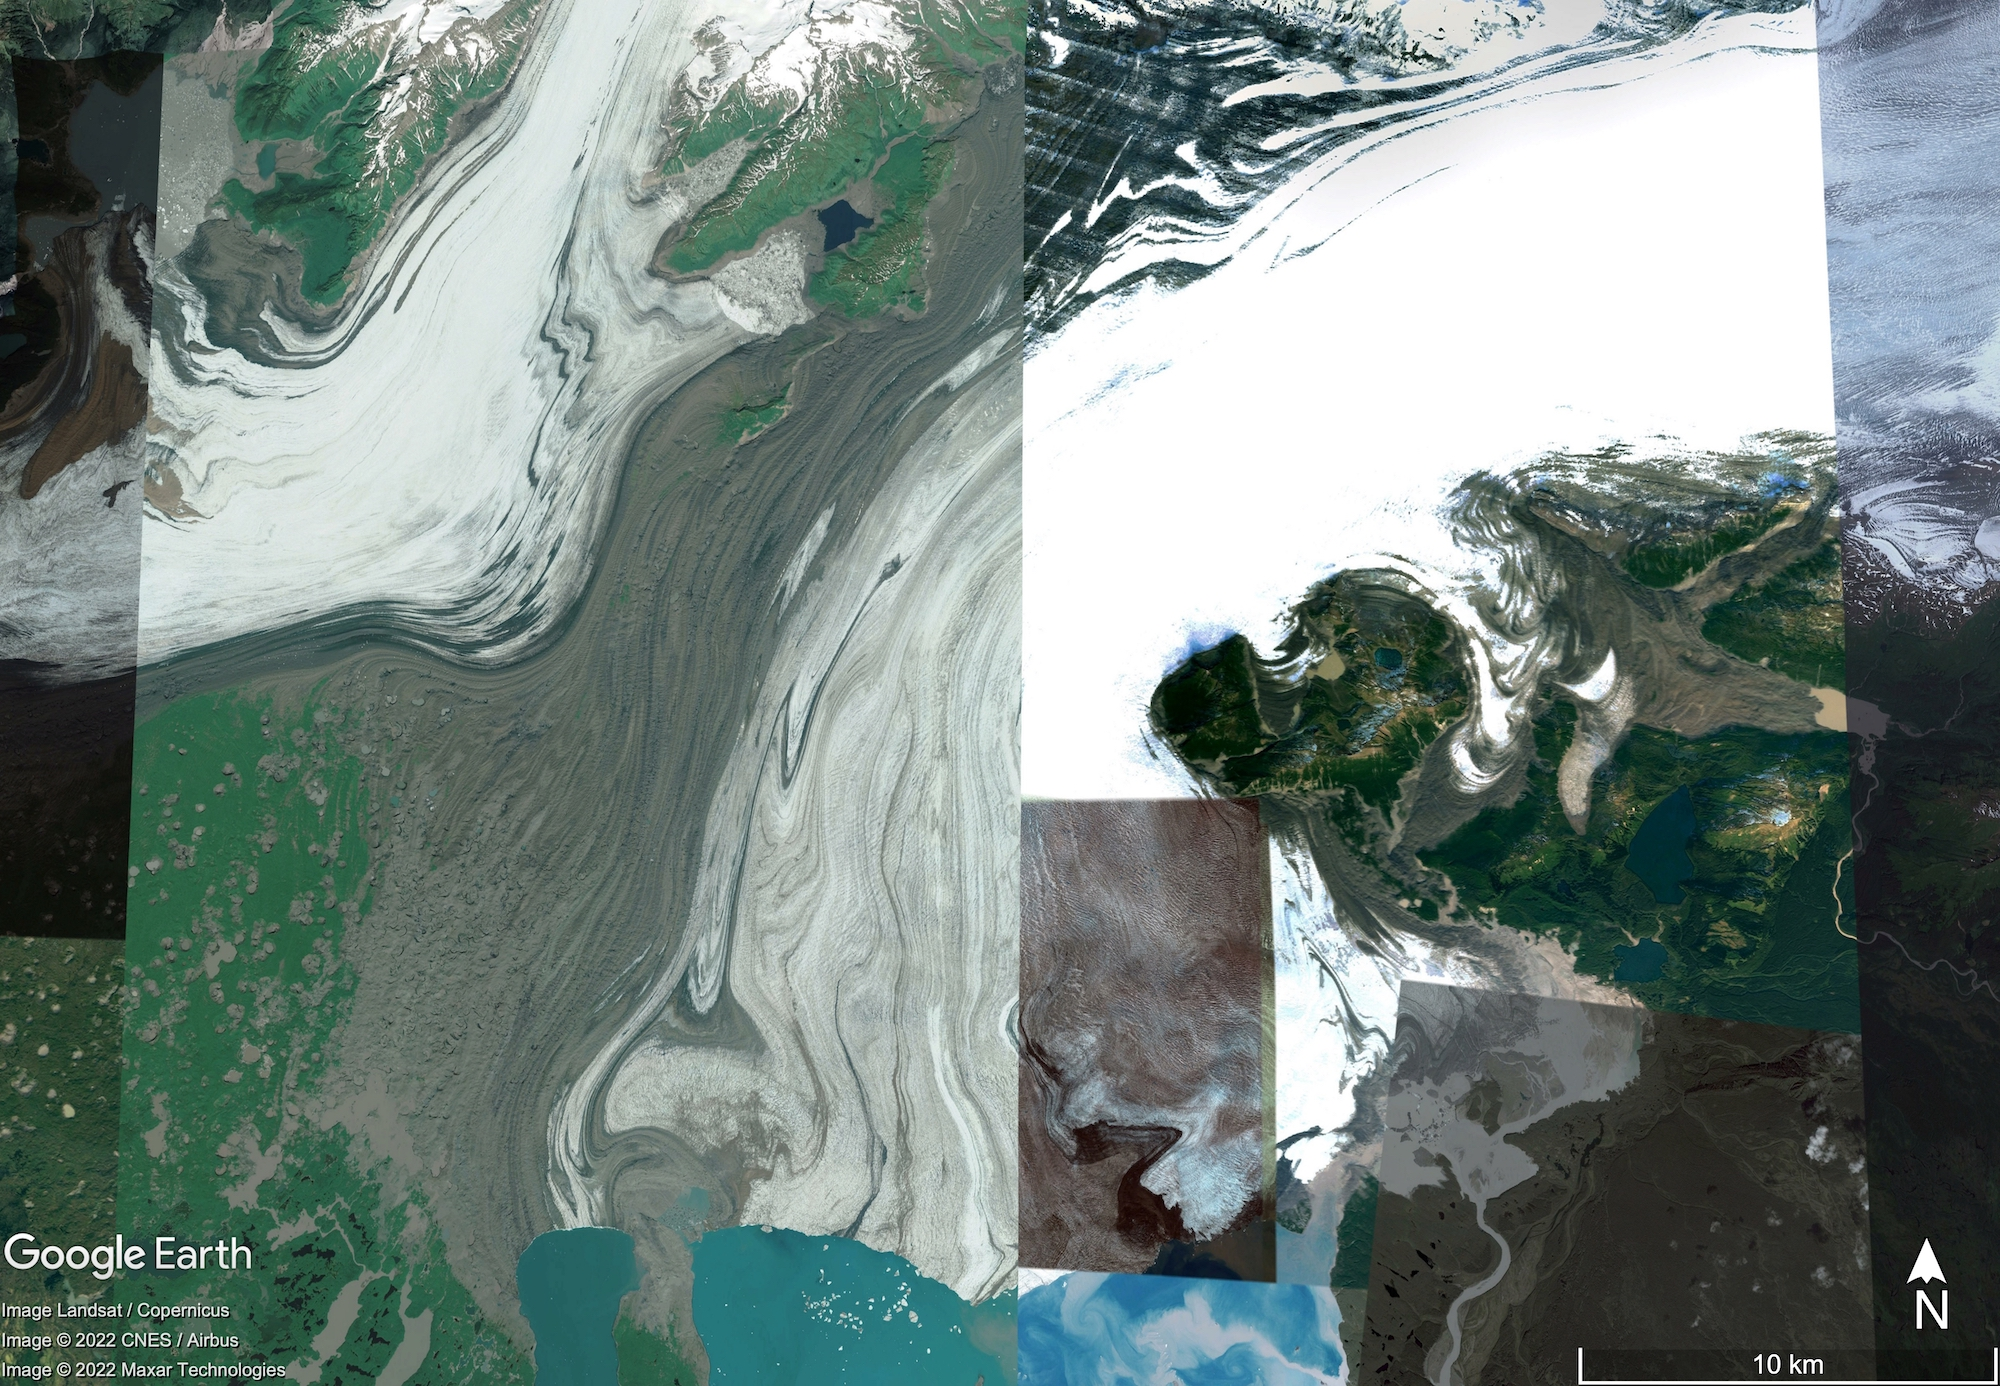
\includegraphics[width=0.48\textwidth]{Alaska4.jpg}} \\
		\subfloat[\label{fig:glacier2}]{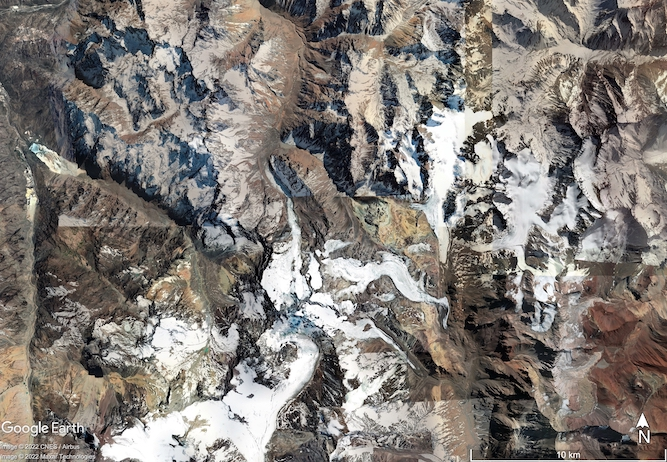
\includegraphics[width=0.48\textwidth]{Andes1.jpg}} 
		\caption{Satellite imagery of \textit{(a)} Bering Glacier, Alaskan Gulf, and \textit{(b)} Juncal Glacier, Chile . For \textit{(a)} it is expected that there is no vegetation and the grid box to be primarily ($\gtrsim 90 \%$) dominated by ice. For \textit{(b)} the updated V20 fields specify a $\gtrsim 25 \%$  glacier fraction. Evidently, the V20 fields for these grid boxes are insufficiently accurate or informative, as identified by VESPER.} 
		\label{fig:glacier}
	\end{figure}
	
	%\begin{figure}[h!]
	%
	%	\subfloat[\label{fig:cvh2}]{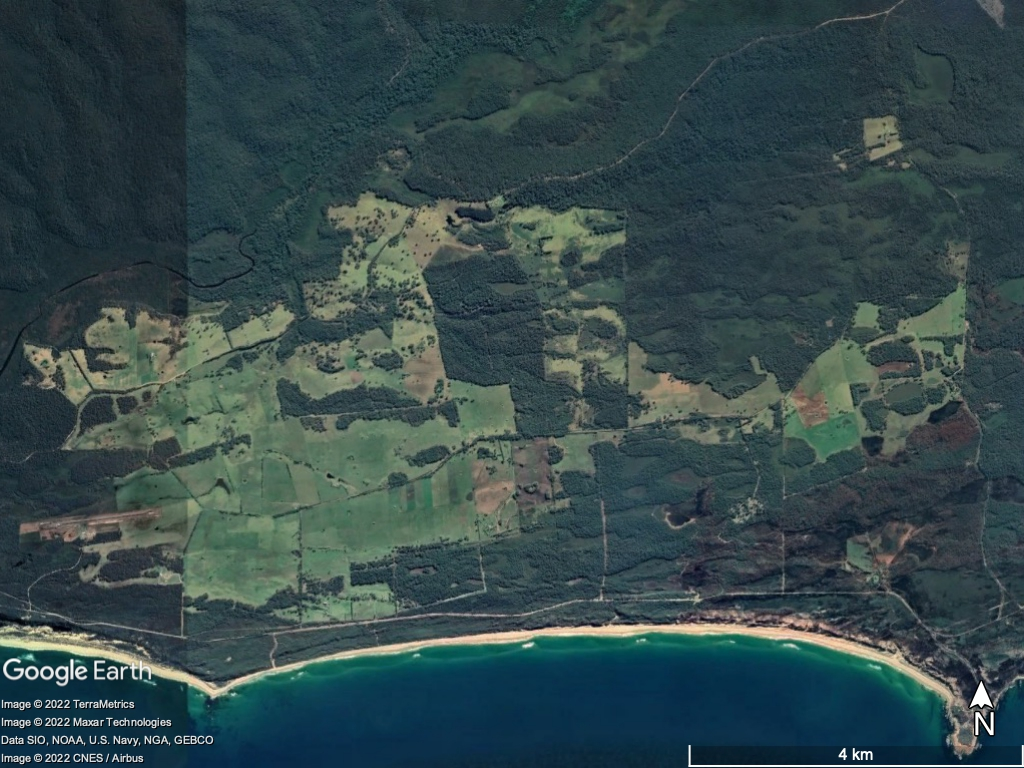
\includegraphics[width=0.48\textwidth]{australia_googleearth.jpg}} \\
	%	\subfloat[\label{fig:cvh3}]{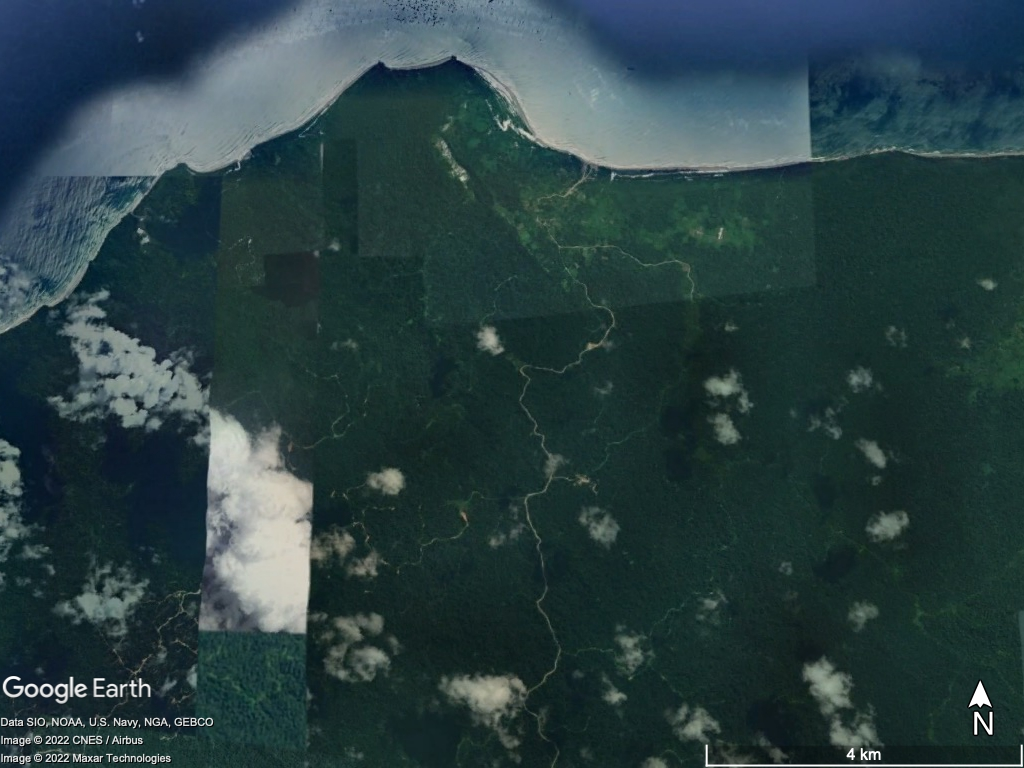
\includegraphics[width=0.48\textwidth]{cvh_hr.jpg}} \\
	%	\subfloat[\label{fiig:cvh1}]{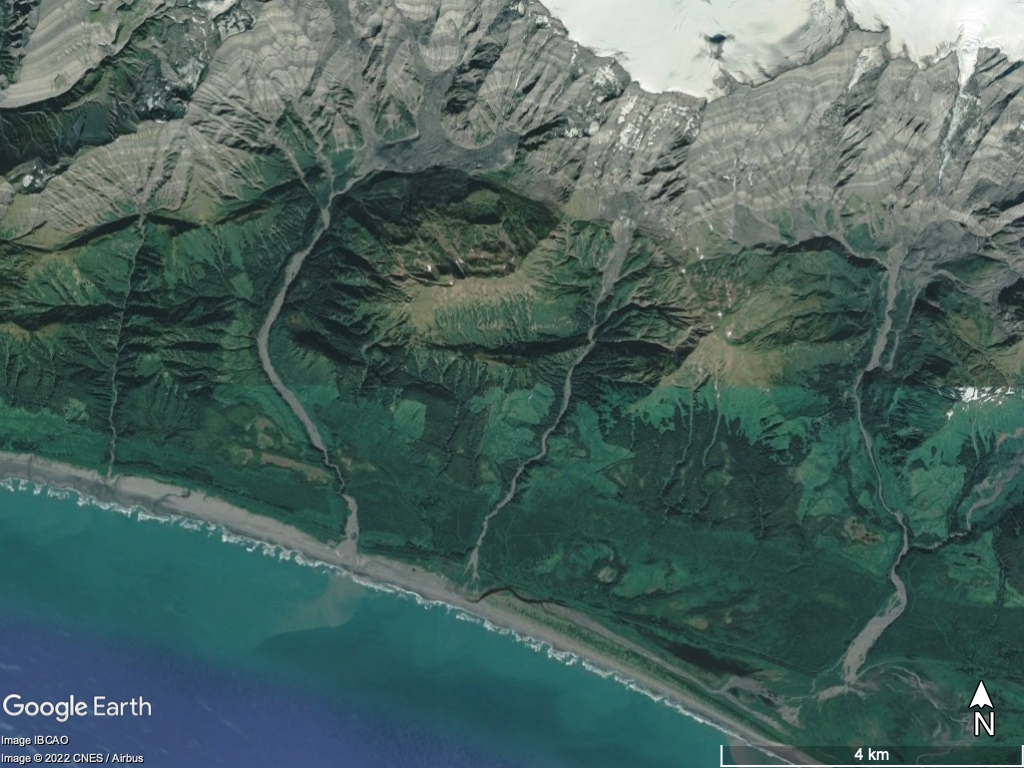
\includegraphics[width=0.48\textwidth]{alaska_googleearth.jpg}} 
	%	\caption{Satellite imagery of grid boxes in \textit{(a)} the Southern coast of Victoria, Australia, \textit{(b)} Siberut Island, Indonesia  and \textit{(c)} the Alaskan Gulf. For \textit{(a)} and \textit{(b)} it is expected according to the updated V20 fields that there is no vegetation, just bare ground. For \textit{(c)} it is expected that there is no vegetation and a large fraction of ice.  Evidently, the V20 fields for these grid boxes points are insufficiently accurate, as identified by VESPER. } 
	%	\label{fig:cvh}
	%\end{figure}
	
	\noindent From this example deploying VESPER on the lake parametrisation fields, it is evident that VESPER enables the user to quickly identify regions where the new parametrisation works effectively (e.g. Aral Sea) as well as spotting regions where it is less performant (e.g. Lake Natron, high vegetation updates). In turn, those areas where the predictions do not improve as expected can be inspected and erroneous or sub-optimal representations of the surface fields identified. This then provides key information on how to introduce further corrections to better represent these more difficult or complex regions. We will now further explore some of these problematic areas and demonstrate how VESPER can guide the development and introduction of additional surface fields.
	
	
	
	\subsection{V20X: Monthly water \& salt lakes}
	\noindent Particular regions where it was difficult for the model to make predictions - especially with the updated V20 fields which only include permanent water - were either areas with a large degree of temporal variability (e.g. lakes which flood and dry out periodically, or freeze and melt) or else lakes which are salt water rather than fresh water lakes. Clearly if the size, shape and depth of a lake are changing over the course of the year, these are going to be hugely significant factors in modelling the lake temperature response. Similarly, saline lakes behave very differently to fresh water lakes since increased salt concentrations affect the density, specific heat capacity, thermal conductivity, and turbidity, as well as evaporation rates, ice formation and ultimately the surface temperature. These two properties of time variability and salinity are often related; it is common for saline lakes to flood and dry out over the course of the season, which naturally also affects the relative saline concentration of the lake itself.  \newline 
	
	
	\noindent Currently, neither the V15 or V20 models have any information regarding the salinity of the lakes or their time variability. Indeed, FLake is specifically a fresh water lake model! We can introduce this information by also including a global salt lake map and monthly inland water lake map as input features,  and use VESPER to investigate the added value of these additional fields.  To create a monthly inland water map we first create 12 monthly fractional land sea masks based on JRC Monthly Water History v1.3 maps for 2010-2020. Since the annual lake maps were created taking into account a lot of additional sources we enforce the extra condition on the monthly maps that the monthly water is equal or greater than permanent water distribution from fractional land sea mask. To create an inland salt water map we used the salt lake list from GLDBv3. First, in order to identify separate lakes on inland water map, we mask small sub-grid lakes and large lake coasts, i.e. grid-cells that have water fraction less than 0.25. Next, we compute number of connected grid-cells in each lake (i.e. connected with sides only). Then we vectorise only lakes that have 100 and more connected grid-cells, as at ERA5 resolution of $\sim$ 31 km the grid-cells are quite large and can include a mixture of freshwater and saline lakes. Finally, saline lake vectors are selected by filtering vectors which have no saline lake point located from GLDBv3. This process resulted in a map at ~31 km resolution based on 147 large salt lake vectors. In the future we plan to revisit the map of salt lakes and extend the list to include additional data. \newline 
	
	
	
	\noindent We create a new model iteration ``V20X" which is analogous to the V20 model, but now also has as input features the monthly water (a quasi-time variable field) and the salt lake cover (a static field). We again train the model on 2016 and make predictions for 2019. The results are presented alongside the V20 results in Table \ref{tab:V1520_results}. \newline 
	
	\subsubsection{Category: Lake Updates}\label{V20XLake}
	
	\noindent We can see that for the Lake Updates category, the prediction accuracy averaged over the year is effectively unchanged from the V20 model. For the Lake-Ground Updates category, the accuracy has decreased slightly, from $\delta_{\rm V20} = -1.12$ K to $\delta_{\rm V20X} = -1.09$ K, although the difference is so small as to be within the model noise. The equivalence of the annually averaged V20X and V20 models is something that we will return to later in Section \ref{sec:timeseries} when we consider the time-variability of the prediction error. If for now instead of a globally averaged metric, we focus on the problematic points that we discussed previously, then V20X demonstrates a significant improvement over V20 for all considered grid points, as illustrated in Table \ref{tab:lake_v20X}. 
	\begin{table*}
		\centering
		\begin{tabular}{lccc}
			Grid Point & $\delta_{\rm V20}$ (K) & $\delta_{\rm V20X}$ (K)  & $\delta_{\rm V15X}$ (K) \\
			\hline
			Lake Natron, centre       & 5.40 & 2.80  & 0.68 \\
			Lake Natron, north          & 1.66 & 1.54   & 1.10 \\
			Lake Blanche                  & 1.79  & -0.64 & 2.76 \\
			Great Salt Lake Desert  & 1.78  & -0.28  &-0.86  \\
			Afghanistan                     & 1.66 & -0.38  & -0.16 \\
			Northern India                 & 1.60 &0.59  & -5.87 \\
			Toshka Lakes                  & 1.56 & -0.59 & -0.14 \\
			\hline
		\end{tabular}
		\caption{$\delta_{\rm M}$ values for selected grid points within the Lake Updates category for each of the trained V20/V20X/V15X models. V20X consistently outperforms V20 at these locations, but for some points, e.g. Lake Natron, underperforms the more basic V15 model. Conversely, V15X underperforms V20/V20X globally, but can outperform V15 at some selected points, where the updated V20 fields are less accurate.}
		\label{tab:lake_v20X}
	\end{table*}
	For Lake Blanche, V20X reduces the prediction error by 2.43K compared to V20. This is in-spite of the fact that our salt lake maps do not identify Lake Blanche as a salt lake, and so all the improvement in the prediction is from the additional information from the monthly lake maps. The salt lake maps are similarly inaccurate for the grid point in Northern India, failing to recognise the underlying salt marsh. However, again the information contained in the monthly lake maps allows the reduction in the error by $2.19$K. There are also regions where the saline maps are correct to not specify any salinity, such as in Afghanistan and the Toshka lakes; again the monthly maps provided sufficient information to allow for a marked improvement by $2.04$ K and $2.15$ K respectively. This is particularly notable since the size of the monthly lake corrections is small for these points: the mean monthly correction for Afghanistan is 0.046 and for the Toshka Lakes is 0.001. However, under the updated V20 both of these areas have had all water removed and so adding in just a small amount of time variable water allows for much more accurate predictions. This example illustrates how VESPER both can identify inaccurate fields and quantify the value of updated fields, as well as emphasizing the importance of time variable lake fields more generally. For points where the saline maps do specify that the underlying lakes are salt lakes - Lake Natron and Salt Lake Desert - it is not possible to disentangle whether the gain is due to the saline maps or the monthly maps. The centre of Lake Natron exhibits a particularly notable improvement by $2.6$K, whilst for the grid point on the northern edge the gain is more modest at $0.12$K. This is likely due to the fact that the updated monthly maps provided much stronger corrections at the centre of the lake (mean correction 0.13) than at the northern edge (mean correction 0.02). For the grid point at the Great Salt Lake Desert, the improvement is $2.06$ K again with a strong correction from the monthly lake maps (mean value 0.16) and the salt maps (mean value 0.56). This improvement is to be expected given the known strong salinity and time variability in the region, and so it is a nice confirmation to have these updated fields verified by VESPER. It is also notable that the variation in the monthly lake maps at this point is very large, with a standard deviation in the lake fraction over 12 months of 0.18. At the start of the year the corrections from the monthly maps are very large, then as the year progresses the magnitude of the corrections generally decreases as the lake dries out. Such a large variation is again difficult to ever capture with a static field. \newline 
	
	\noindent Other regions of note that we have mentioned previously are the Northwest Territories and the Nunavut province in Northern Canada where the V20 model underperformed relative to V15, with $\delta_{\rm V20} = +0.02$ K. The introduction of the monthly lake maps modestly improves the predictions in this area, with $\delta_{\rm V20X} = -0.03$K.  In these high latitude regions one might expect some time variability due to freezing and thawing of the lake surfaces, and the addition of the monthly lake maps to the model then provides some of this time variable information, allowing for improved predictions.  Whilst this is an improvement, the effect is modest; it is generally difficult to get quality observations at high latitudes, especially during the cold season, due to increased cloud cover. Therefore whilst VESPER can say that the addition of the monthly lake maps does improves the predictions in these regions, for improved performance cloud independent data should be used.  Additionally, the corrections from the monthly lake maps are small in these regions, with a mean correction of 0.02 and a generally small variance; in actuality time variable fields with greater variance over the year may be more accurate. Due to the freezing and thawing, improving ice on/off date prediction by the lake parametrisation should help better describe the seasonality and variance. \newline 
	
	\noindent It is worth emphasising that whilst the V20 and V20X models are improvements over V15 globally, and V20X is generally an improvement over V20 for these problematic points, there are regions where neither V20 or V20X outperform V15 ($\delta_{\rm M}$ is always positive), such as Lake Natron and Northern India. Given all the extra information provided to the more advanced models this is unusual, unless the additional information is erroneous in these regions or else the temperature response is completely atypical to the rest of the globe and the additional information is not predictive in these regions. To explore this hypotheses we train one further model, V15X. This is analogous to V20X, being simply the V15 model with the additional monthly maps and salt lake fields included. Importantly it does not have the updated correction fields from V20. Globally, this model performs worse that the V20 models, as we might expect - for example in the Lake Updates category $\delta_{\rm V15X} = -0.25$K compared to $\delta_{\rm 20X} = -0.45$ K. However, V15X does perform well at these problematic points (see Table \ref{tab:lake_v20X}). For both the Lake Natron grid points V15 outperforms V20X, suggesting that at this location the V20 fields are generally less accurate than the V15 fields. V15X however underperforms relative to V15 which also indicates that the monthly maps and the salt lakes are either inaccurate at this location, or that the temperature response of Lake Natron is highly atypical. For Northern India, the performance of the V15 model is particularly striking; whilst the V20 and V20X models struggled to make more accurate predictions than V15, V15X decreases the average prediction error by nearly 6K. This again indicates that for this point the V20 fields are less accurate than V15. Similarly for the Great Salt Lake Desert, $\delta_{\rm V20} = 1.78$ K, $\delta_{\rm V20X} = -0.28$ K but $\delta_{\rm V15X} = -0.86$ K, which suggests that whilst the monthly lake maps and the salt lake fractions are accurate and informative in this area, the static V20 fields are not. These examples illustrates again how VESPER can identify particular regions where the fields are inaccurate, as well as emphasising the need more generally for accurate descriptions of seasonally varying inland water and saline lake maps in Earth system modelling.  \newline 
	
	
	\subsubsection{Category: Vegetation Updates}
	Whilst the Vegetation Updates category explicitly deals with areas where the lake fraction does not change when going from V15 to V20, many of the grid points in this category do contain some kind of waterbody, often lying close to the coast or else containing lakes or large rivers. Information on the salinity and temporal variability of these water bodies can then  influence the prediction accuracy. By providing the additional information in V20X, the mean $\delta_{M}$ is reduced from $\delta_{\rm V20} = +0.049$K to $\delta_{\rm V20X} =0.005 $K. This performance is gained despite the known errors for some of the grid boxes in the \textit{cvh} vegetation updates (e.g. Figure \ref{fig:cvh}), again demonstrating the importance of salinity and seasonally varying water. The V15X model is less performant than V20X, with $\delta_{\rm V15X} = 0.11$K since there \textit{are} some grid boxes in this category where the updated V20 fields are accurate and valuable if augmented by monthly variability. However if we consider just the worst performing grid points where $\delta_{\rm V20} > 1$ K then the mean values are $\delta_{\rm V20} = 2.0$ K, $\delta_{\rm V20X} = 0.49$ K and $\delta_{\rm V15X} = 0.21$K. This again demonstrates how the \textit{cvh} fields have been erroneously updated for a small selection of grid points in V20. 
	
	
	\subsubsection{Category: Glacier Updates}
	We would expect the additional information provided by V20X to be particularly effective for glacial grid points. Glacier ice is naturally found next to waterbodies which freeze and thaw over the year, and the salinity of water will also influence this freezing. Therefore accurate additional information from the monthly lake maps and the saline maps should prove useful in these more time variable regions. This is indeed what we observe with the mean delta going from $\delta_{\rm V20} = -0.13$K to $\delta_{\rm V20X}= -0.24$K.  Considering the two problematic points that we discussed previously, in the Alaskan Gulf the prediction accuracy relative to V15 has improved from $\delta_{\rm V20} = +2.16$ K to $\delta_{\rm V20X}= +1.00$ K, whilst for the Juncal Glacier the prediction accuracy has also improved, with $\delta_{\rm V20X}$ decreasing to $+1.88$ K. Despite this improvement, again for both of these points the prediction accuracy still lags behind V15. This is on account of the V20 fields being insufficiently accurate in these areas, as has been discussed. Neither of these grid points correspond to saline lakes or have a significant time variability in the monthly lake fractions and so are also not improved by a V15X model.
	
	%For the Alaskan Gulf, the improvement through the introduction of the monthly lake maps (salt fields here are zero) suggests that again this is a grid point where the variability in the surface water strongly influences the skin temperatures. Indeed, this grid point lies at a high latitude ($\sim 60^{\circ}$ N) where the surface will freeze and thaw over the course of a year, naturally influencing the surface water fraction. For the Kerguelen Islands, the V20X prediction is still worse than V15. If we deploy V15X then the error is strongly reduced to $-0.91$. This again is good evidence that the updated V20 surface fields, such as the glacial fraction are less accurate for this particular grid point.
	
	
	
	\subsubsection{Timeseries}\label{sec:timeseries}
	
	
	\noindent Thus far we have been focusing mainly on the $\delta_{\rm M}$ metric averaged over the entire year of the test set. It is also of interest to explore how the prediction error for each of the 3 models varies with time. This is demonstrated in Fig \ref{fig:timeseries} for each of the 4 updated categories that we have discussed. \newline  
	
	\noindent For the Lake Updates and Lake-Ground Updates categories we can see that all the model predictions track the same general profile, with the error peaking in the northern hemisphere summer months. This is a result of FLake modelling being least accurate during the summer as the lake is not fully mixed and so the mixed layer depth for lakes is too shallow, resulting in skin temperatures with larger errors. Conversely, in the autumn and spring the lake is fully mixed and predictions have the smallest errors compared with observations. A clear hierarchy of models is evident; the V20/V20X models consistently outperform the V15 model across the year. This again is solid evidence, highlighted by VESPER, of the value of the updated fields both static and seasonally varying. We mentioned previously how the annually and globally averaged $\delta_{\rm M}$ values for the Lake Updates category were highly comparable for V20 and V20X, despite V20X significantly improving the worst behaving points. We can see from the top panel in Figure \ref{fig:timeseries} that the V20X model is a systematic improvement on V20 from around April onwards, but at earlier times in the year V20 outperforms V20X. This is likely for two reasons. Firstly, the monthly lake maps are in fact a climatology and therefore insufficiently precise to detect the exact ice on/off dates during the winter months, where we have a large number of grid points at high latitudes which will be subject to freezing, nullifying any time variability. Secondly, due to the accuracy of the lake mean depth which strongly drives the ice on-dates due to its influence on the heat capacity of the lake. During the warmer months lakes thaw, the monthly maps are more accurate, as the thawing of lake ice is mainly connected to the atmospheric conditions, not the lake depth, and so the information contained in them can be used to make more accurate predictions. The Lake-Ground Updates timeseries broadly follows the same general profile as Lake Updates, but the errors are larger - those grid points where the lakes have been replaced with bare ground were particularly poorly described in V15. Additionally, for Lake Updates we see two sharp decreases in the prediction error during $\sim$ April and September, which are not as strongly reflected in Lake-Ground. This is due to the geographic location of the grid points in each of the two categories; for the Lake Updates category the grid points are located primarily in the boreal zones and so are subject to freezing and thawing over the course of the year leading to a strong seasonality due to the lake mixing that we have discussed. The sharp drop in April corresponds to a time where the lakes are unfrozen and fully mixed. However the lakes in the Lake-Ground sub-category are less concentrated and much more evenly distributed over the globe and so do not exhibit such a strong seasonality. \newline 
	
	
	
	\noindent Examining the timeseries for Vegetation Updates, whilst there is a large degree of variability, we again see the trend previously discussed whereby the V20 fields make the predictions systematically worse across the entirety of the test year. The introduction of the monthly lake maps in V20X compensates for the erroneous V20 vegetation fields - the V20X predictions are generally worse than V15 at the start and end of the year, but better in the middle. This is due to the fact that the majority of the points in the Vegetation Updates category are in climate zones which have pronounced rainy and dry seasons e.g. Indonesia, the Amazon. At the start of the year during the wet season there is lots of precipitation and the static V15 fields are generally more accurate. As the rains abate and the dry season starts the V15 lake fields are underestimates which are then improved through the introduction of additional water via the monthly lake maps. \newline 
	
	
	
	\noindent For Glacier updates we can separate grid points into the northern and southern hemispheres. We again consider just those points where the number of MODIS observations at a given instant in time, per ERA data point is greater than 50. For the northern hemisphere the familiar hierarchy of models is recovered, with the V20X model generally outperforming V20, which in turn generally outperforms V15. The errors peak for all models in the summer, again due to the lakes not being fully mixed. There is also an uptick in the prediction error for all models during the winter when the freezing is greatest - this indicates how ice cover can strongly influence the land surface temperature response. For the southern hemisphere the story is different. The errors are smallest during the middle of the year when we expect the freezing to be greatest. During the spring and autumn the errors are largest - this is correlated with a decrease in the number of observations suggesting that this is due to poorer data quality due to cloud cover. In the summer when the weather is clearer the errors start to decrease again. Given this variation in the data quality due to cloud cover it is difficult to draw any strong conclusions, and again for stronger performance cloud independent data should be used. What is obvious for the southern hemisphere glacier grid points is that the V20 and V20X models struggle to improve on V15, unlike in the northern hemisphere. This suggests that the updated V20 fields are still insufficiently accurate for southern latitudes. \newline 
	\begin{figure}
		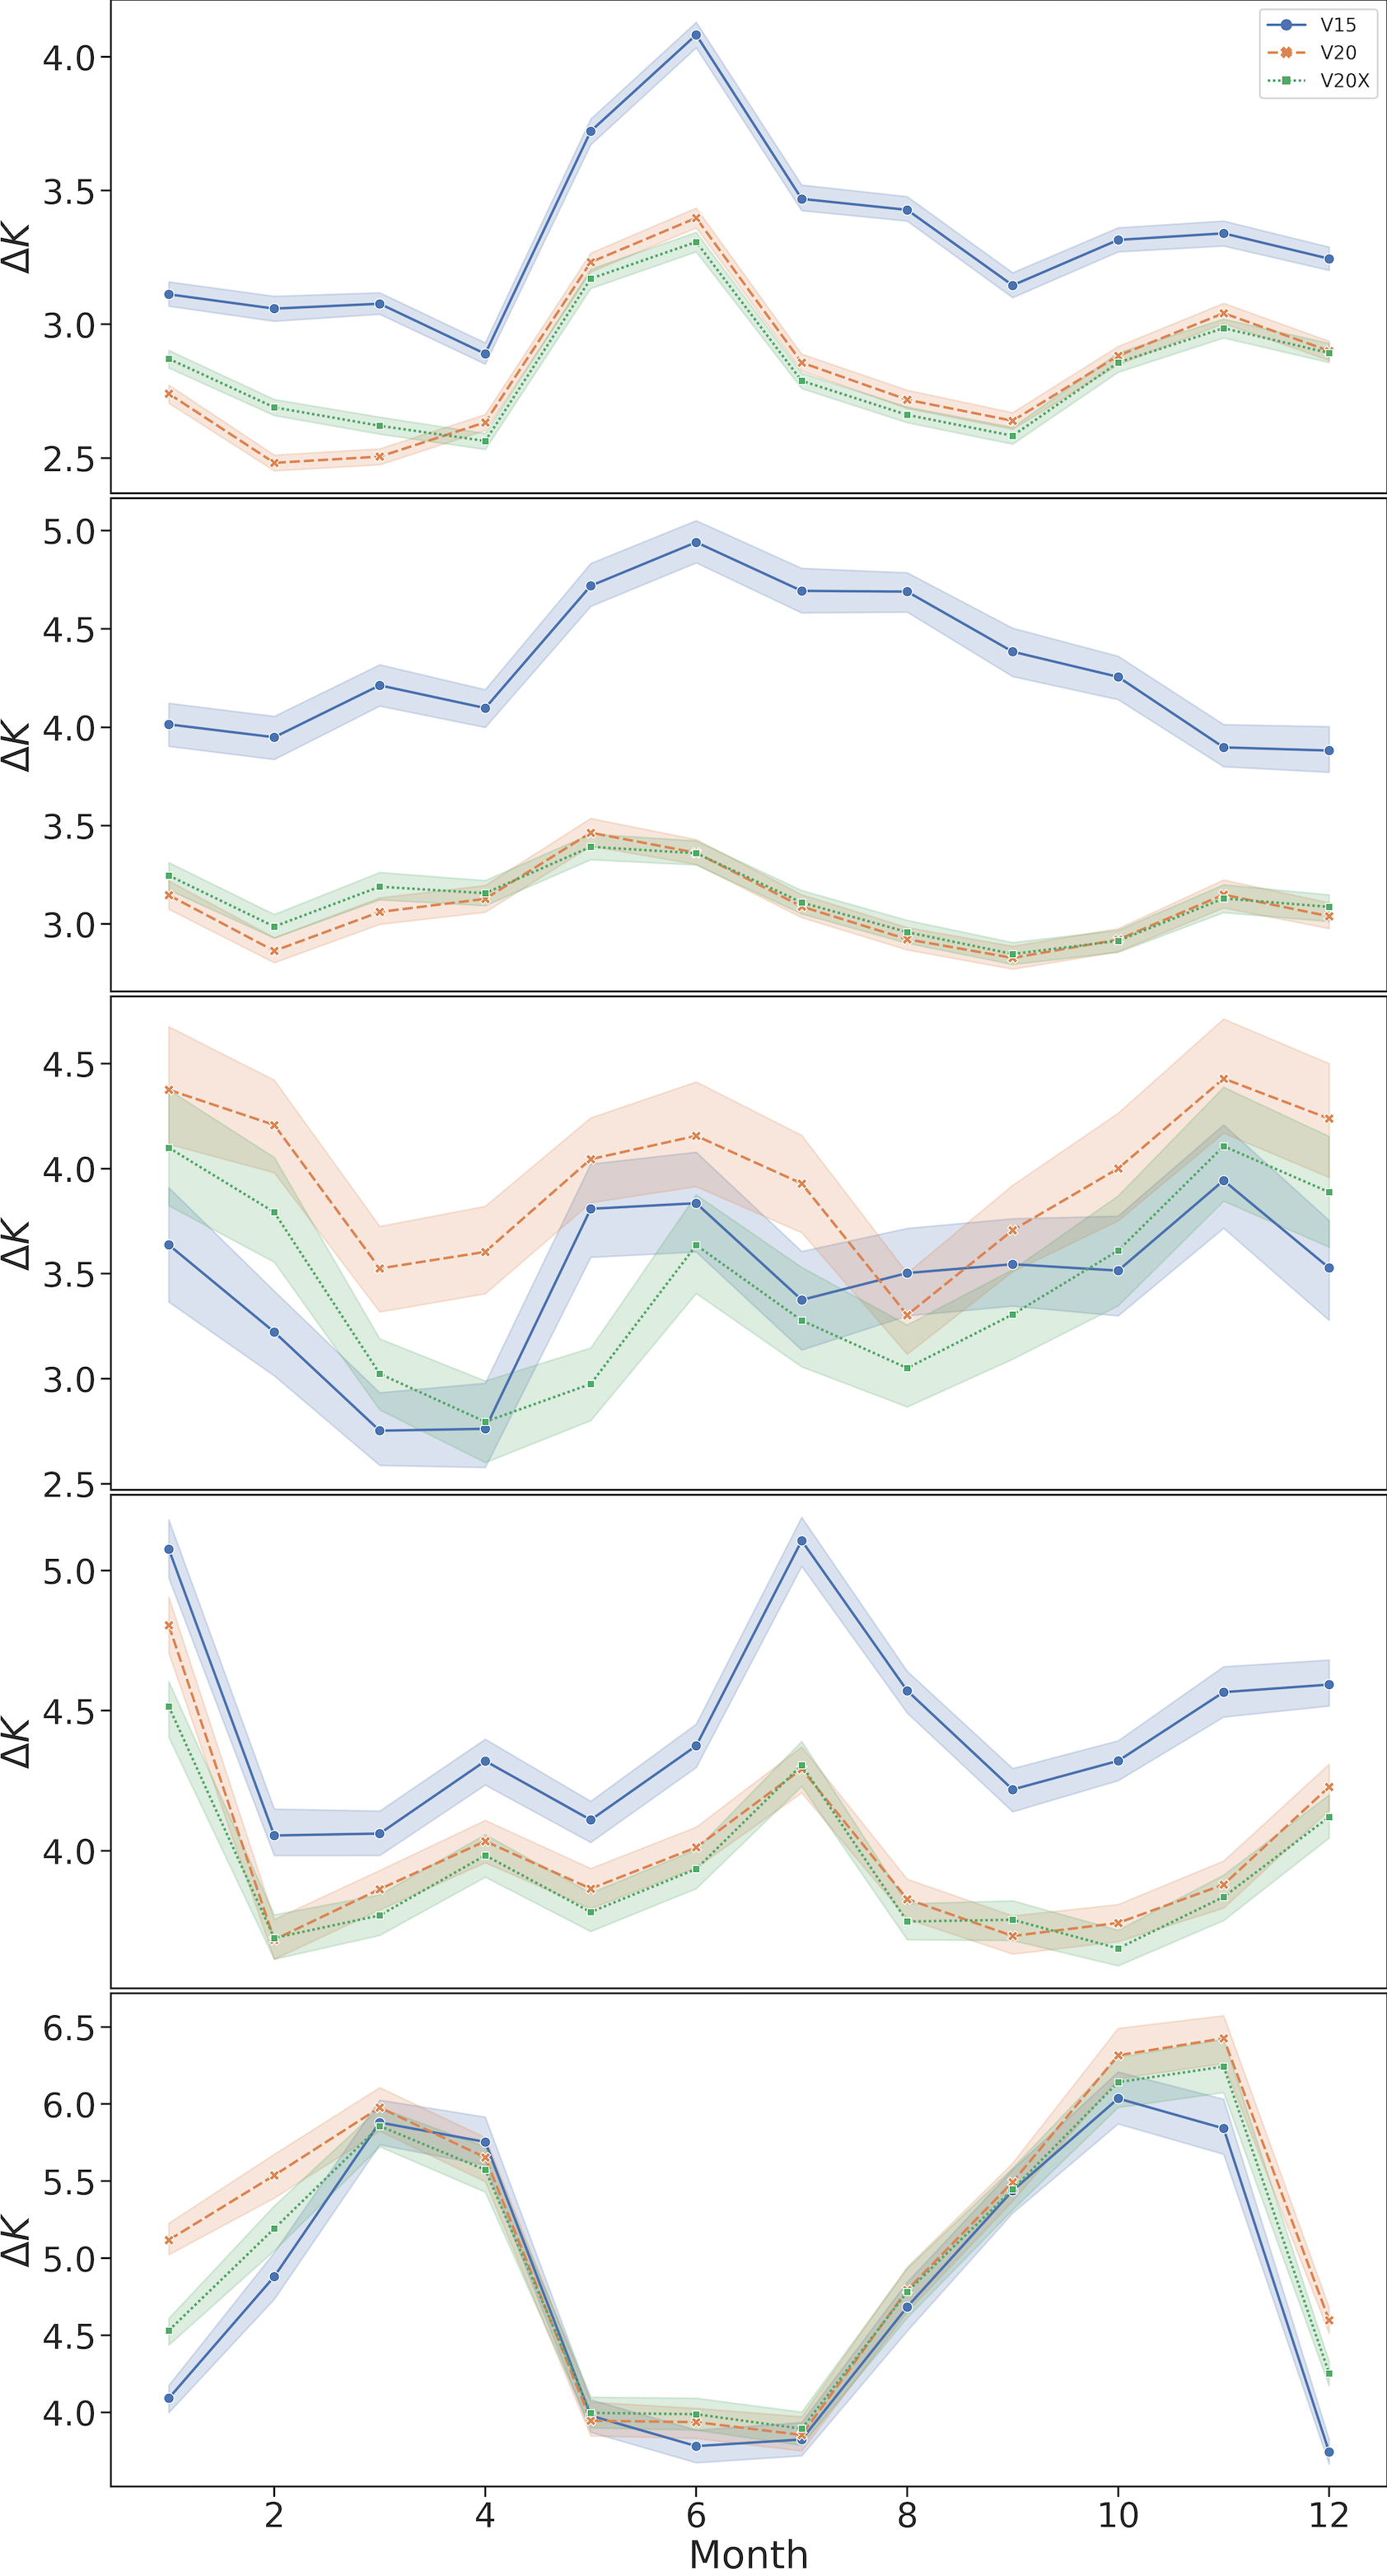
\includegraphics[width=\columnwidth]{mega_stack_ns.png}
		\caption{Mean prediction error in the surface temperature $\bar{\Delta} K$, averaged over all grid points, for each of the 3 models over the course of the test year for (\textit{top panel}) Lake Updates, (\textit{second panel}) Lake-Ground Updates, (\textit{third panel}) Vegetation Updates, (\textit{fourth panel}) Glacier Updates, northern hemisphere and (\textit{bottom panel}) Glacier Updates, southern hemisphere. For the Glacier Updates category we again exclude grid points where the number of MODIS observations per ERA data point is less than 50.  For the Lake categories, all models follow the same general profile, with the V20X model generally outperforming the V20 model over the year, which in turn outperforms the V15 model. The value of the additional V20 correction fields and the V20X monthly lake maps and salt lake maps, is evident.}
		\label{fig:timeseries}
	\end{figure}
	
	
	\noindent We have also discussed previously particular grid points where there is expected to be a large degree of temporal variability or the lakes are saline and as a consequence the static V15/V20 fields struggle to make accurate predictions (e.g. Table \ref{tab:lake_v20X}). In Figure \ref{fig:timeseries_stacked} we present timeseries for two of these points: Lake Natron in Tanzania and Gujarat Province, India. Both these points were discussed in Sections \ref{V20Lake} and \ref{V20XLake}. We can see that for these two selected points the hierarchy of models no longer holds. Whilst there is a large degree of variability, and there is no clear separation between models that we get when averaging over all grid points as in Fig \ref{fig:timeseries}, generally it can be seen that the V20 model performs the worst, indicating that the updated fields are not accurate in these regions. For Lake Natron the V20/V20X models are significantly worse throughout almost the entire year. The updated models - which specify a much larger lake fraction than in V15 - perform well at the beginning and start of the year which tend to be the wettest months at Lake Natron. However,  during the summer as the lake dries out the errors grow significantly. This indicates again that the updated V20 fields are in fact over-corrections for this area. Similarly, whilst the V15X model is a significant improvement over V20/V20X - since it does not have these inaccurate fields -  it is still less performant than the basic V15 again due to the additional water that V15X specifies. Together this strongly indicates that there is little surface water at Lake Natron during 2019. \newline 
	
	
	\noindent For Gujarat Province in Northern India the story is different. Now the V20 model is systematically worse than V15 over the entire year, indicating that the static V20 fields are less accurate than the V15 fields. The V20X model shows a strong time variability, with the errors being smallest in the summer which is the wet season in Gujarat and largest in the winter which is the dry season. This suggests that the monthly maps are most accurate during the summer, providing extra information which is missing from V15/V20, but may be overestimates during the winter. The V15X model has a notably strong performance, outperforming the other models almost every month. This again is further evidence of the inaccuracy of the V20 fields and the value of the time-variable monthly water information.
	\begin{figure}
		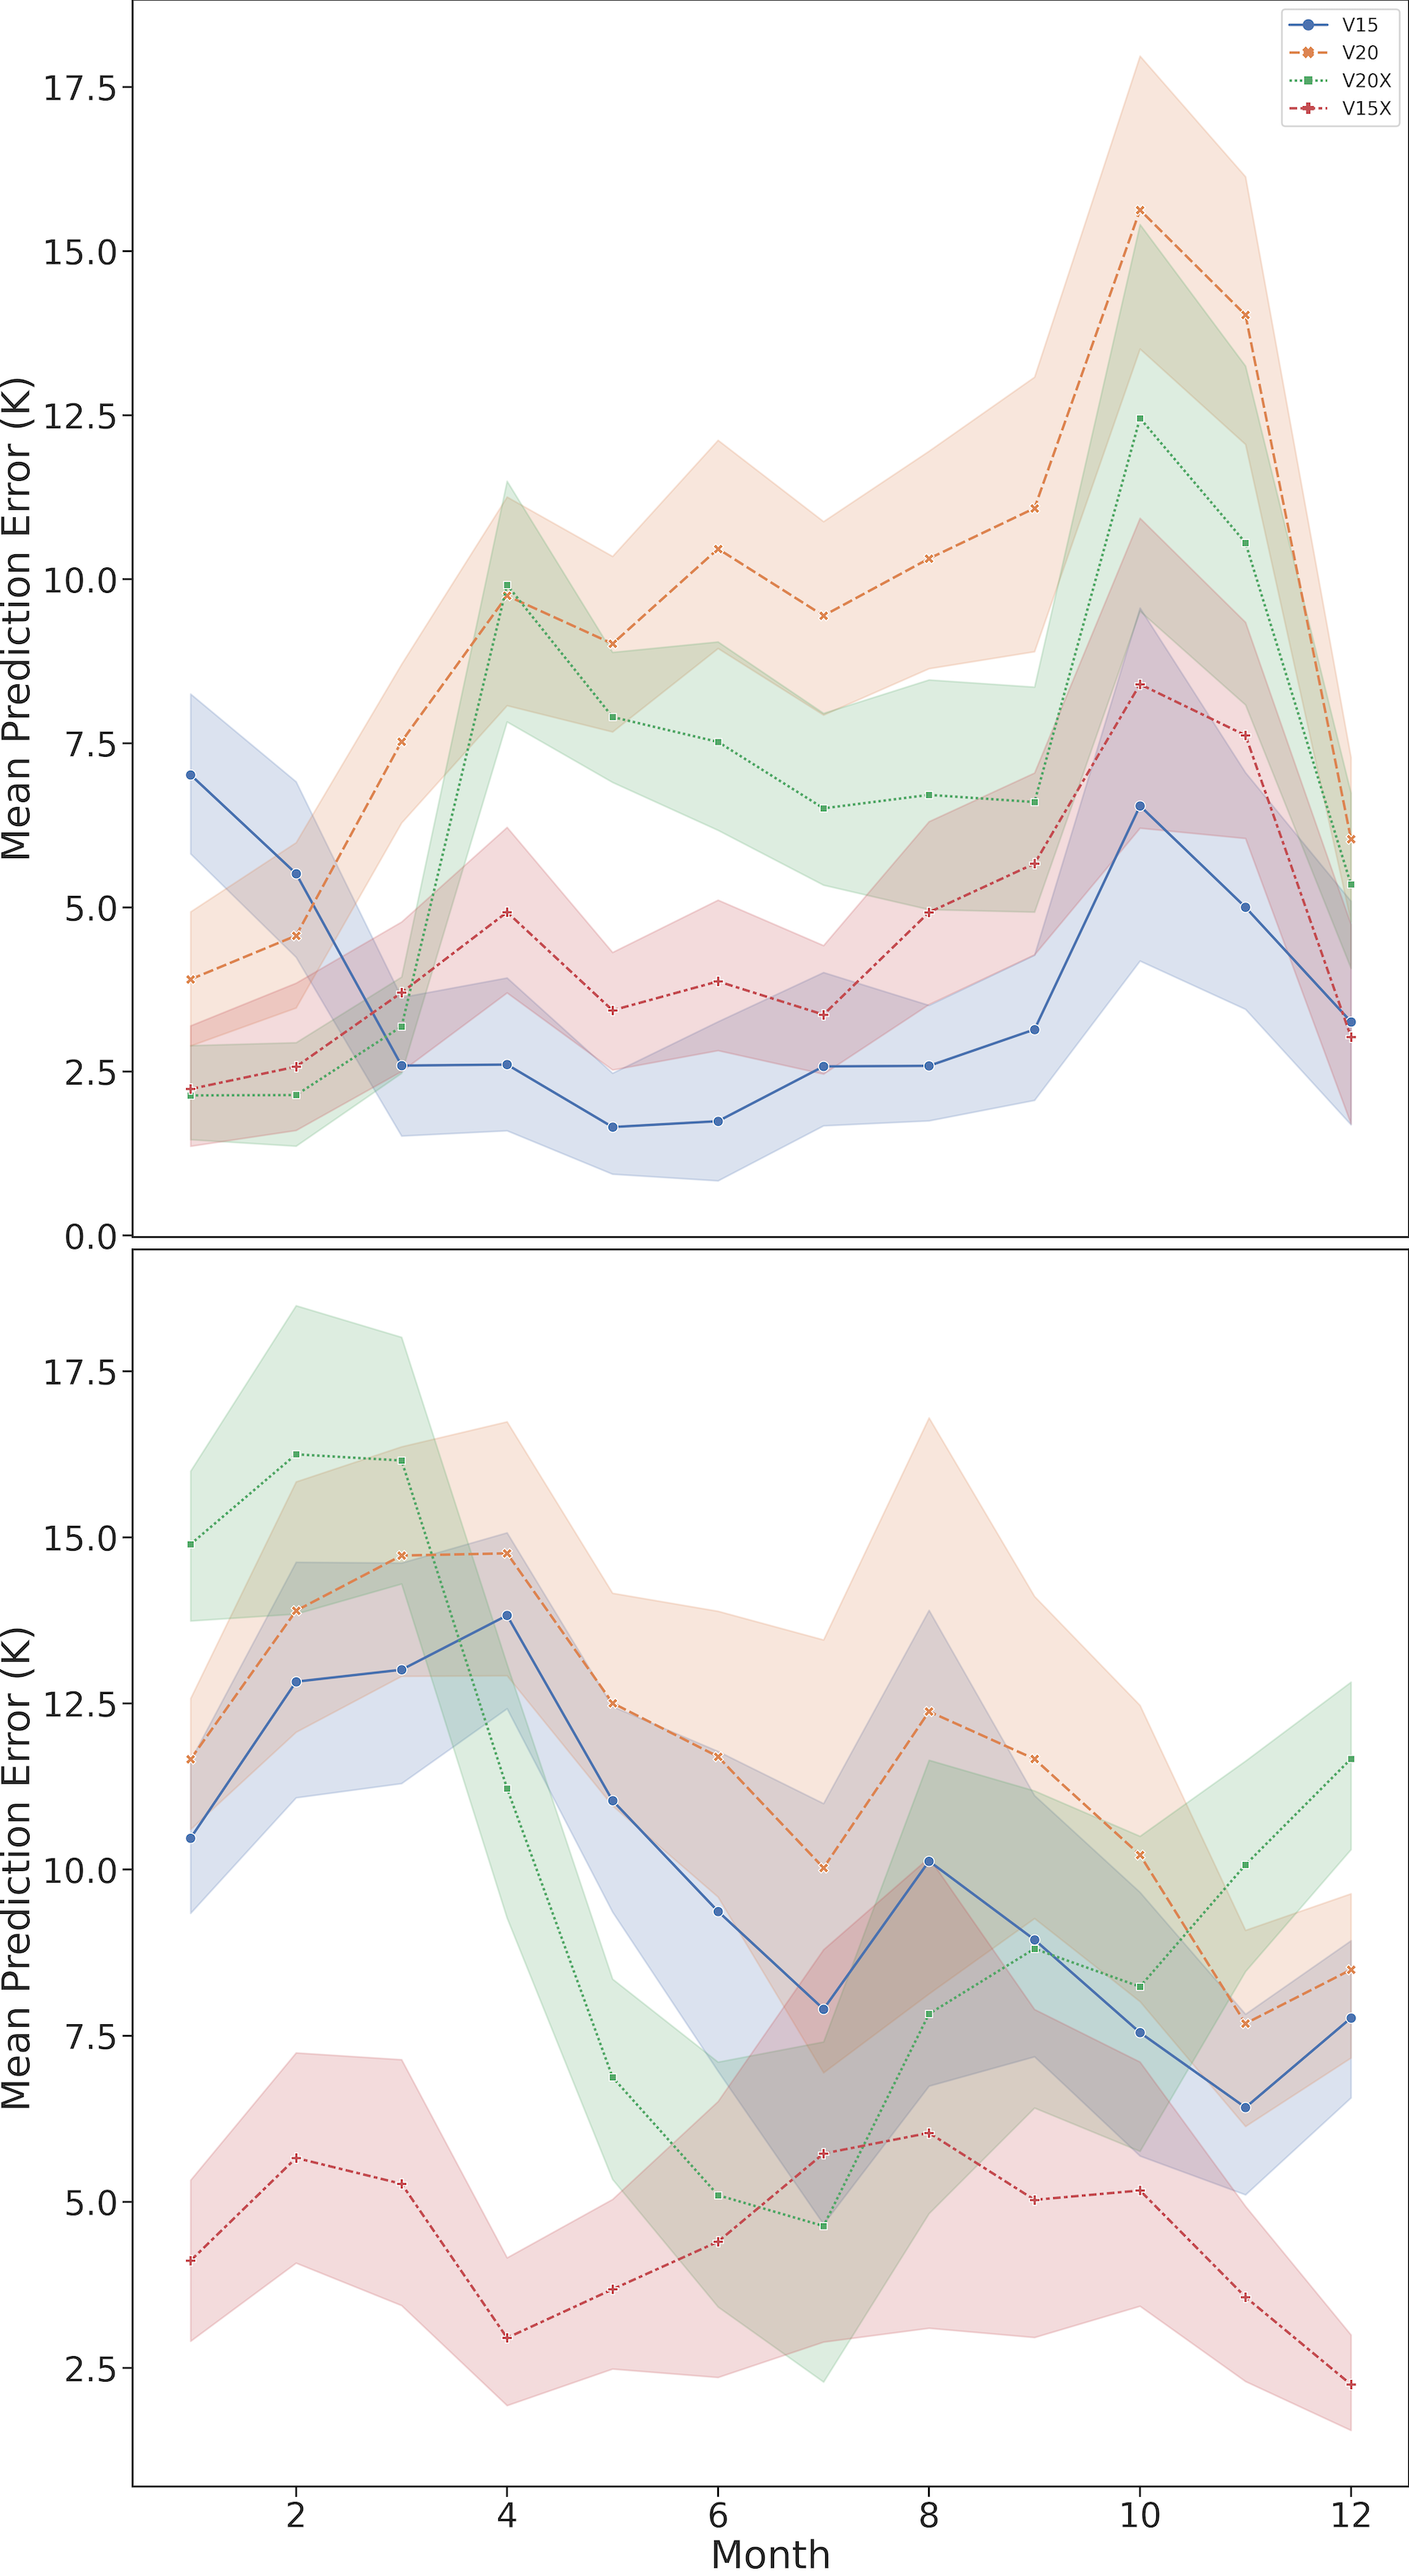
\includegraphics[width=\columnwidth]{stacked_timeseries_lakes_new.png}
		\caption{Variation in the prediction error for the grid points at Lake Natron, Tanzania (top panel) and Gujarat Province, India (bottom panel). There is a large degree of variability, but for Lake Natron the V20 and V20X models are generally less performant than V15 and V15X, indicating that the updated V20 fields are less accurate here. The augmented models with saline and monthly lake maps outperform those without, indicating the value of these fields in these regions.} 
		\label{fig:timeseries_stacked}
	\end{figure}
	
	\section{Discussion} \label{sec:4}
	We have seen how VESPER can quantitatively evaluate the value of updates to the lake surface parametrisation as well as identifying areas where the updates are insufficiently accurate. For the former VESPER was able to show that the major regions where the lake surface parametrisation fields were updated - such as the Aral sea - enjoyed more accurate predictions, which verifies both the accuracy of the fields and their information content with respect to predicting skin temperatures. For the latter VESPER was able to identify grid points where the predictions became worse with the updated fields, indicating that the updated fields were in fact less accurate. More generally we have also seen how detailed knowledge of surface water fields (e.g. up to date permanent water distribution, seasonal water distribution, salt lake distribution, etc.) can notably improve the accuracy with which the skin temperature can be modelled, e.g. grid points with significant updates (i.e. where the field has changed by $\geq$ 10 \%) to the lake fields show a mean absolute error reduction of skin temperature globally of $0.45$K (Table \ref{tab:V1520_results}). 
	
	
	\noindent There are multiple possible further extensions of this work. We have not currently included the errors on the MODIS observations into the VESPER model. During the ``matching-in-space" step relating the ERA and MODIS data (Section \ref{sec:join}), it could be a worthwhile extension to weight the averaged MODIS points by their corresponding errors (e.g. Fig. \ref{fig:MODIS_obs_error}) when deriving a single MODIS observation for a given ERA grid point. This would then provide a more accurate and confident representation of the true surface temperature at a particular space-time point. Due to the inherent stochasticity of training a model it is also possible for different models to settle in different local minimas i.e. the network variance. It would also be desirable to train an ensemble of models (``ensemble learning") and combine the predictions from multiple models to reduce this variance. We have focused here primarily on hydrological applications, our primary concern being the ability to evaluate the parametrised water body representation, however the method would work generally for any updated fields that we want to assess. Extension to non-lake hydrological fields like wetland extant or river bathymetry model parameters, or even non hydrological fields such as orography would be an interesting further development. The development of a more mature, integrated pipeline for automatically evaluating updated parametrisations could also be a worthwhile pursuit. Another natural extension of this work which may prove fruitful in the enterprise for improved parametrised representation of water bodies is to invert the problem and treat VESPER as a function to optimise. That is to say, VESPER can be thought of as a function which takes some inputs - in this case a lake parametrisation - and returns a loss metric i.e. how accurate the predictions are compared to the test set. Given this loss metric it may then be possible to vary the inputs and use standard optimisation techniques to learn the optimal parametrisation. Whilst this may be an expensive technique as there are effectively two nested models over which to optimise (for every optimisation step in the higher model, one must train the VESPER network from scratch) it could be possible given appropriate hardware or with reduced data focusing just on targeted locations (e.g. \textit{``What is the best way to represent the lakes in this area?"}). The loss gradient information can also be used to tune individual features, informing  whether an input variable should be larger or smaller. 
	
	
	\section{Conclusion}\label{sec:conclusion}
	Weather and climate modelling rely on accurate, up-to-date descriptions of surface fields, such as inland water, so as to provide appropriate boundary conditions for the numerical evolution. Lakes can significantly influence both weather and climate, but sufficiently accurate representation of lakes is challenging and the natural changes in water bodies mean that these representations need to be frequently updated. A new method based on a neural network regressor for automatically and quickly verifying the updated lake fields - VESPER - has been presented in this work. This tool has been deployed to verify the recent updates to the FLake parametrisation, which include additional datasets such as the GSWE and updated methods for determining the lake depth from GLDBv3. The updated parametrisation fields were shown globally to be an improvement over the original fields; for a subset of grid points which have had significant updates to the lake fields, the prediction error in the skin temperature decreased by 0.45K. Conversely, VESPER also identified individual grid points where the updated lake fields were less accurate, enabling these points to subsequently be corrected, such as losing forests to bare ground leading to errors of 1.1K.  Multiple further extensions of this work, including extension to non lake fields and the development of a more mature integrated pipeline have been discussed.
	
	\section{Code}
The code used in constructing VESPER, including the methods for joining the ERA and MODIS datasets and the construction of the neural network regression model is open-sourced at \url{https://github.com/tomkimpson/ML4L}
	
	
	\section{Acknowledgments}
	This project has received funding from the European Research Council (ERC) under the European Union’s Horizon 2020 research and innovation programme (Grant No 741112).
	
	
	
	%\conclusions  %% \conclusions[modified heading if necessary]
	%TEXT
	
	%% The following commands are for the statements about the availability of data sets and/or software code corresponding to the manuscript.
	%% It is strongly recommended to make use of these sections in case data sets and/or software code have been part of your research the article is based on.
	
	%\codeavailability{TEXT} %% use this section when having only software code available
	
	
	%\dataavailability{TEXT} %% use this section when having only data sets available
	
	
	%\codedataavailability{TEXT} %% use this section when having data sets and software code available
	
	%
	%\sampleavailability{TEXT} %% use this section when having geoscientific samples available
	%
	%
	%\videosupplement{TEXT} %% use this section when having video supplements available
	
	
	%\appendix
	%\section{}    %% Appendix A
	%
	%\subsection{}     %% Appendix A1, A2, etc.
	%
	%
	%\noappendix       %% use this to mark the end of the appendix section. Otherwise the figures might be numbered incorrectly (e.g. 10 instead of 1).
	
	%% Regarding figures and tables in appendices, the following two options are possible depending on your general handling of figures and tables in the manuscript environment:
	
	%% Option 1: If you sorted all figures and tables into the sections of the text, please also sort the appendix figures and appendix tables into the respective appendix sections.
	%% They will be correctly named automatically.
	
	%% Option 2: If you put all figures after the reference list, please insert appendix tables and figures after the normal tables and figures.
	%% To rename them correctly to A1, A2, etc., please add the following commands in front of them:
	
	%\appendixfigures  %% needs to be added in front of appendix figures
	
	%\appendixtables   %% needs to be added in front of appendix tables
	
	%% Please add \clearpage between each table and/or figure. Further guidelines on figures and tables can be found below.
	
	

	
	%\disclaimer{TEXT} %% optional section
	

	
	
	%% REFERENCES



\newpage
%%%%%%%%%%%%%%%%%%%%%%%%%%
%BIBLIOGRAPHY
\bibliographystyle{ieeetr}
\bibliography{refs}
%\begin{thebibliography}{refs}
%\bibitem{}
%\end{thebibliography}

\end{document}